\documentclass[12pt]{article}

\usepackage[margin=0.5in, includefoot]{geometry}
\usepackage{setspace}
\usepackage{titlesec}
    \titleformat{\subsubsection}{\normalfont\normalsize\itshape}{\thesubsubsection}{1em}{}
\usepackage{hyperref}
\usepackage{xurl} % yay this works
    \hypersetup{
        colorlinks=true, 
        linkcolor=blue, % can comment this out if the blue figure faces is bothersome
        urlcolor=cyan
    }
    \renewcommand{\figureautorefname}{\textbf{Figure}} % decent fix but later should figure out how to make numbers bolded too
\usepackage{enumitem}
    \setlist[enumerate]{label=(\arabic*)}
\usepackage{amsmath}
\usepackage{amssymb} % for mathfrak font style
\usepackage{mathrsfs} % for mathscr font style
\usepackage{cancel}
\usepackage{xfrac}
\usepackage{array}
\usepackage{multicol}
\usepackage{float}
\usepackage[many]{tcolorbox}
    \definecolor{cellborder}{HTML}{CFCFCF}
    \definecolor{cellbackground}{HTML}{F7F7F7}
\usepackage{listings}
    \lstset{
        basicstyle=\scriptsize\ttfamily, % font style
        escapeinside={(*@}{@*)} % escape into LaTeX using (*@ and @*)
    }
\usepackage{subcaption}
\usepackage{wrapfig}
\usepackage{graphicx}
\usepackage{multirow}
\usepackage{csvsimple}
\usepackage[font=small]{caption}
\usepackage{xcolor} % for formatting purposes
\usepackage{lipsum} % for formatting purposes
% \usepackage[hang, flushmargin]{footmisc} % seeing if default setup is actually nice looking

\renewcommand{\thesubsection}{\arabic{subsection}}
\newcommand{\displayinline}[1]{\displaystyle#1\mathstrut}
\newcommand{\totder}[2][]{\frac{\mathrm{d}#1}{\mathrm{d}#2}} % needs amsmath package
\newcommand{\parder}[2][]{\frac{\mathrm{\partial#1}}{\mathrm{\partial#2}}} % needs amsmath package
\newcommand{\thetadot}{\dot{\theta}}
\newcommand{\thetaddot}{\ddot{\theta}}
\newcommand{\g}{\;\mathrm{g}}
\newcommand{\s}{\;\mathrm{s}}
\newcommand{\Hz}{\;\mathrm{Hz}}
\newcommand{\radian}{\;\mathrm{rad.}}
\renewcommand{\Re}{\mathfrak{Re}} % these are just cooler
\renewcommand{\Im}{\mathfrak{Im}}
\newcommand{\im}{\mathrm{i}}
\newcommand{\diff}[1]{\text{d}#1}
\newcommand{\R}{\mathbb{R}}

\newsavebox\foobox
\newlength{\foodim}
\newcommand{\slantbox}[2][0]{\mbox{%
        \sbox{\foobox}{#2}%
        \foodim=#1\wd\foobox
        \hskip \wd\foobox
        \hskip -0.5\foodim
        \pdfsave
        \pdfsetmatrix{1 0 #1 1}%
        \llap{\usebox{\foobox}}%
        \pdfrestore
        \hskip 0.5\foodim
}}
\def\Lagrangian{\slantbox[-0.2]{$\mathcal{L}$}} % ok wow nailed it (I think?)
\def\Fourier{\slantbox[-0.45]{$\mathscr{F}$}} % kinda legible yeah

%%%%%%%%%%%%%%%%%%
% begin document %
%%%%%%%%%%%%%%%%%%
\begin{document}
\setstretch{1.15}

\section*{Lagrangian Formalism and Fast Fourier Transform of Coupled Pendulums}

\begin{quote}
    Jeff Lam \\
    \textit{Department of Physics, Binghamton University} \\
    March 14\textsuperscript{th}, 2025
\end{quote}

\subsection*{Abstract}
A coupled pendulums setup was studied under the perspective of:
(1) Lagrangian mechanics for understanding the complex theory behind the system's motion; and (2) Fast Fourier Transform (FFT) for
relative ease in deriving the constituent frequencies that make up a given oscillation.
From the Lagrangian, the system's equations of motion are derived as $\theta_1(t)=c_1\cos(\omega_1t)+c_2\cos(\omega_2t)$ and $\theta_2(t)=c_1\cos(\omega_1t)-c_2\cos(\omega_2t)$ for suitable constants $c_1$ and $c_2$,
where $\displaystyle{\omega_1=\sqrt{\frac{g}{\ell}}}$ and $\displaystyle{\omega_2=\sqrt{\frac{g}{\ell}+2\frac{k}{m}}}$.
A FFT application was developed in Python to take \texttt{.csv} exported data and comprehensively plot:
(1) raw, unaltered data; (2) data truncated at the time of oscillation and seperated as individual subplots for a cleaner view;
(3) FFT graph of signal vs. frequencies for viewing and determining peak frequencies.
Several coupling settings were studied for the beat frequencies of the coupled pendulums; $\omega_1$ is reported to be $7.39172\pm0.01191$ $\sfrac{\radian}{\s}$,
with a 7.075\% error when compared to the theoretical value of 7.956 $\sfrac{\radian}{\s}$ as given by the measured values,
while $\omega_2$ as differing in value for 9 cm, 9$\sfrac{1}{2}$ cm, and 10 cm couplings was reported as 8.412 $\sfrac{\radian}{\s}$, 8.855 $\sfrac{\radian}{\s}$, 8.531 $\sfrac{\radian}{\s}$,
which do not proportionally follow the coupling strength of the system given the rubber band position.
The antisymmetric mode of the coupled pendulum was also studied, with a guess on the trend towards the ideal FFT graph for a proper antisymmetric mode trial run as the only result reported.


\noindent\rule{\linewidth}{0.5pt}

\begin{multicols}{2}

\subsection{Introduction}
The typical pendulum experiment usually involves oscillating a single, simple pendulum
and approximating its period with a stopwatch--- a well-known classical mechanics experiment
that is straightforward in setup yet rich in theory through the understandings of Newtonian mechanics.
The coupled pendulums experiment as presented in this paper is a much more advanced classical mechanics experiment
in comparison. \textbf{Figure 1} depicts the system as set up in lab as two identical pendulums each having
a bob mass $m$ joined at the end of a stiff yet lightweight shaft of length $\ell$ which is furthermore attached
to a Rotary Motion Sensor (RMS) for electronic gathering of data. 
\columnbreak
\begin{figure}[H]
    \centering
    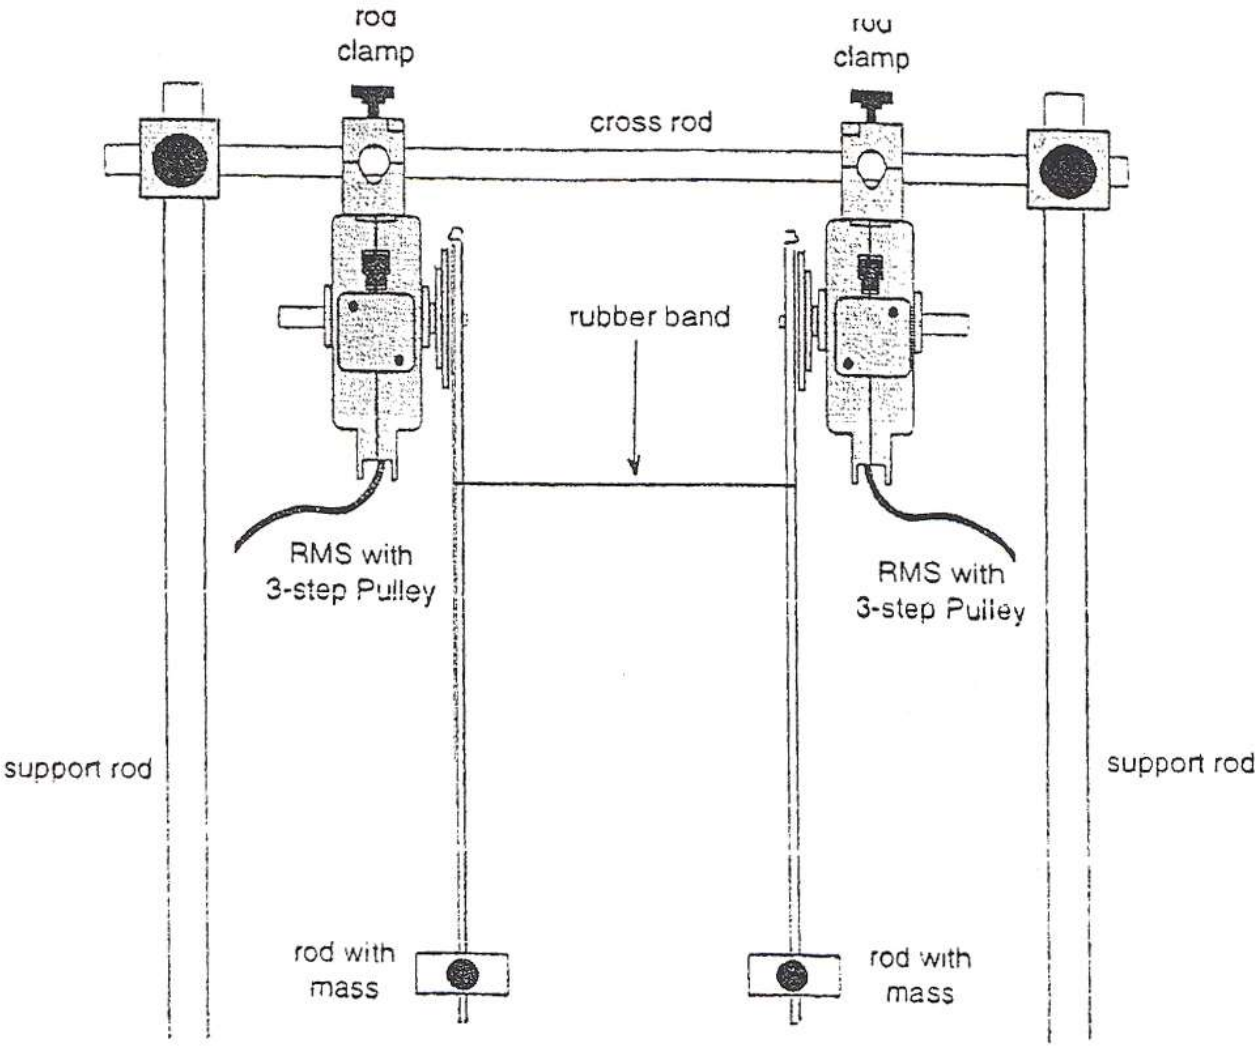
\includegraphics[width=0.95\linewidth]{figs/fig1_cropped.png}
    \caption{Schematic illustration of the coupled pendulums lab setup [\hyperref[sec:1]{1}]}
    \label{fig:1}
\end{figure}
\noindent
The system is ``coupled'' via a rubber band binding the shafts together.

This experiment is a challenge compared to the typical pendulum experiment due to the
need of: (1) analytical mechanics to model each individual pendulum motion; and (2) a different methodology for analyzing
sensor-gathered data as compared to human-approximated period data.
This paper presents solutions to both respective major ideas through: (1) Lagrangian formulation of the system;
and (2) Fast Fourier Transform (FFT) of the sensor data to derive constituent frequencies per pendulum waveform.

\subsubsection{Assumptions}
The coupled pendulums system presented here can easily become more complicated unless certain assumptions are made.

First, the assumption of simple pendulums. In the system, $m$ is assumed to be a point-mass and the shaft of length $\ell$ is assumed to be massless per pendulum.
This avoids the complications of treating each pendulum as more generally a compound pendulum, \textit{i.e.}, $m$ as a point-mass contributes to the torque and angular momentum of the system only
(this is despite the fact that the shafts of the pendulums may act as physical pendulums themselves--- the lightweight nature of their material allows this assumption).

Second, the assumption of one degree of freedom per pendulum. Inheritely, the apparatus exists in ordinary space
(or more formally in mathematics, $\R^3$). Consider the floor of the lab reference frame as the $xy$-plane and height
as the $z$-axis. This means realistically a pendulum may swing with \textit{two} degree of freedom, \textit{i.e.},
its position of motion may be describe using both $x$- and $y$- coordinates. This generalization becomes more imperative when
considering the rubber band coupling as well, for the binding would pull the pendulums within two Euclidean direction rather than one most of the time.
\columnbreak
\begin{figure}[H]
    \centering
    \begin{subfigure}{0.32\linewidth}
        \centering
        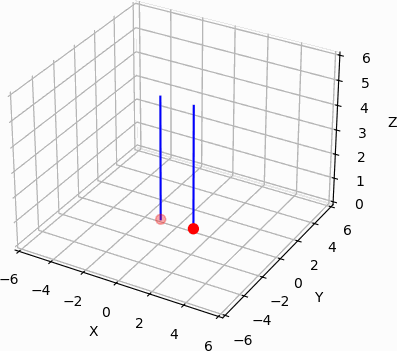
\includegraphics[width=0.98\linewidth]{figs/fig2/a_cropped.png}
        \caption{}
    \end{subfigure}
    \begin{subfigure}{0.32\linewidth}
        \centering
        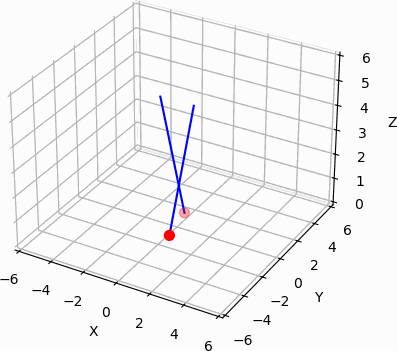
\includegraphics[width=0.98\linewidth]{figs/fig2/b_cropped.png}
        \caption{}
    \end{subfigure}
    \begin{subfigure}{0.32\linewidth}
        \centering
        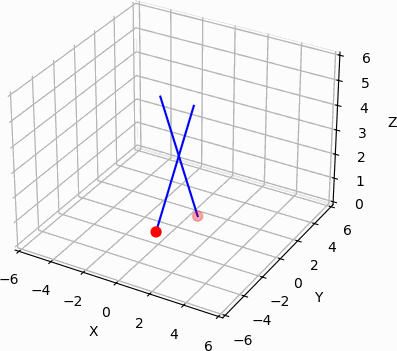
\includegraphics[width=0.98\linewidth]{figs/fig2/c_cropped.png}
        \caption{}
    \end{subfigure}
    \begin{subfigure}{0.32\linewidth}
        \centering
        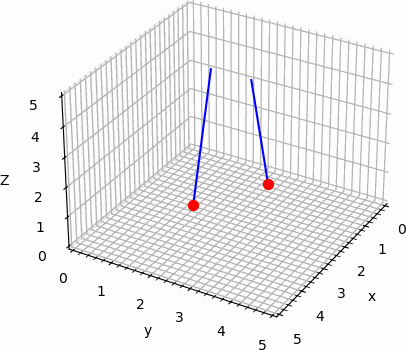
\includegraphics[width=0.98\linewidth]{figs/fig2/d_cropped.png}
        \caption{}
    \end{subfigure}
    \begin{subfigure}{0.32\linewidth}
        \centering
        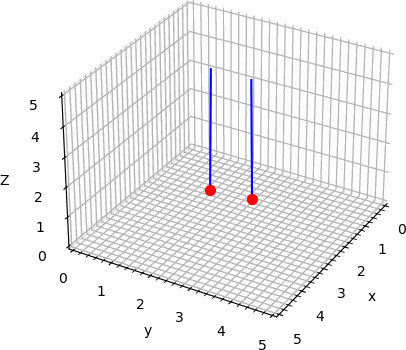
\includegraphics[width=0.98\linewidth]{figs/fig2/e_cropped.png}
        \caption{}
    \end{subfigure}
    \begin{subfigure}{0.32\linewidth}
        \centering
        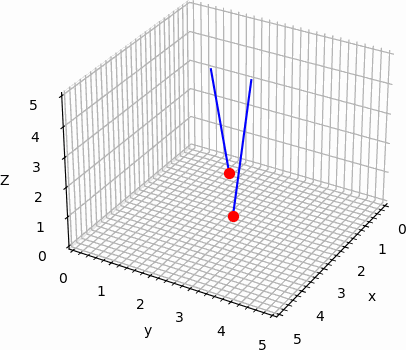
\includegraphics[width=0.98\linewidth]{figs/fig2/f_cropped.png}
        \caption{}
    \end{subfigure}
    \caption{
        Frames of motion for various degrees of freedom.
        (a), (b), \& (c) depicts the pendulums sweeping a circle as an
        example of \textit{two} degrees of freedom motion. (d), (e), \& (f)
        depicts the pendulums swinging simply in parallel to the $x$-axis,
        implying \textit{one} degree of freedom motion.
    }
\end{figure}
\noindent
This assumption asserts then that one of these coordinates be fixed during any given time of a pendulum's motion.
\textbf{Figure 2} provides examples for motions of both one and two degrees of freedoms. 
In the lab setup, the RMS are 3-step pulley systems,
so it is reasonable to assume that each pendulum oscillates within the same \textit{Cartesian plane} (\textit{i.e.},
both pendulum motions swing parallel to a given axis,) for the pulleys' wheels and axles only allow the pendulums to swing in such a fashion.

Third, the assumption of small-angle approximation.
This assumes if the deflection angles for both pendulums are small enough, then $\sin(\theta)\approx\theta$.
The importance of this assumption is made clearer in section \textit{2.2 Small-angle Approximation}.

\subsubsection{An Alternative Approach}
Under the assumptions made in the previous section,
a seperate classical mechanics problem may be presented with the goal of transferring any theoretical analysis available there to the current system shown so far.
\textbf{Figure 3} showcases the alternative coupled pendulums problem, found in a standard upper-undergraduate level classical mechanics textbook.

The assumption of the pendulums oscillating within the same Cartesian plane in the previous section is made useful here as their motion are instead modelled side-by-side in two-dimension,
and an additional assumption of modeling the tension within the rubber band as tension within a spring is made as well.
The additional assumption being made further implies that the energy transfer between the pendulums depicted in either scenario can be modelled by Hooke's Law,
\textit{i.e.}, $U(x)=\dfrac{1}{2}kx^2$.

With all necessary assumptions made and an alternative approach to solving the system analytically and in two-dimensions rather than three,
Lagrangian formalism may now be introduced.


\subsection{The Lagrangian}
\subsubsection{Lagrangian Formulation}
In the given system, the only acting forces are gravity and the spring force, which are both known conservative forces.
By definition then, the Lagrangian of the conservative system is
$$\Lagrangian=T-U$$
where $T$ is the total kinetic energy of the system and $U$ is the total potential energy of the system.

\textbf{Figure 4} illustrates a more proper setup of the alternative coupled pendulums problem (which from now on will be simply referred to as the simplified pendulums problem)---
the most notable change as compared to the illustration in \textbf{Figure 3} is the angles of deflection being represented as $\theta$ rather than $\phi$.
With the proper conventions in place, the following definitions
$$\left\{\begin{aligned}
    T_n &= \frac{1}{2}mv_n^2 \\
    v_n &= r\omega_n
\end{aligned}\right.$$
and proper substitution values (\textit{i.e.}, $r=\ell$ and 
\columnbreak
\begin{figure}[H]
    \centering
    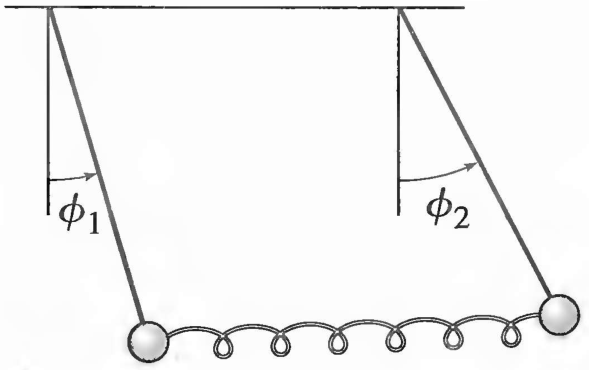
\includegraphics[width=0.98\linewidth]{figs/fig3_cropped.png}
    \caption{
        Alternative coupled pendulums problem as depicted in two-dimensions.
        Adapted from \textit{Classical Mechanics}, by \textit{John R. Taylor} (2003),
        \textit{Figure 11.17} [\hyperref[sec:2]{2}]
    }
\end{figure}
\noindent
$\omega_n\equiv\thetadot_n$) together show that the total kinetic energy of the simplified pendulums problem is
$$T=\frac{1}{2}m\big(\ell\thetadot_1\big)^2+\frac{1}{2}m\big(\ell\thetadot_2\big)^2$$
For the total potential energy of the system, consider first fixing a point of reference as the zero potential.
Let the ceiling where the pendulums are attached to be the reference point for zero potential as according to \textbf{Figure 4}.
Use both $x$- and $y-$ components of either $\ell$'s of the pendulums as defined by
$$\left\{\begin{array}{ll}
    x_1 = \ell\sin(\theta_1), & y_1 = -\ell\cos(\theta_1) \\
    x_2 = \ell\sin(\theta_2), & y_2 = -\ell\cos(\theta_2)
\end{array}\right.$$
as well as $U_n=mgh_n$, where $h_n$ is any given height, as the definition of gravitational potential energy and $U(x)=\dfrac{1}{2}kx^2$ as given by Hooke's Law to define the total potential energy of the simplified pendulums problem as
\begin{multline*}
    V = -mg\ell\cos(\theta_1)-mg\ell\cos(\theta_2) \\ +\frac{1}{2}k\big(\ell\sin(\theta_2)-\ell\sin(\theta_1)\big)^2
\end{multline*}

Thus the formal Lagrangian of the simplified pendulums problem is determined as
\begin{multline*}
    \Lagrangian = \frac{1}{2}m\ell^2\thetadot_1^2 + \frac{1}{2}m\ell^2\thetadot_2^2 + mg\ell\cos(\theta_1) \\
    + mg\ell\cos(\theta_2) - \frac{1}{2}k\ell^2\big(\sin(\theta_2)-\sin(\theta_1)\big)^2
\end{multline*}

\subsubsection{Small-angle Approximation}
Like in the case of the simple pendulum experiment,
where the formal differential equation for its motion,
$$\thetaddot+\frac{g}{\ell}\sin(\theta)=0$$
is nonlinear due to the $\sin(\theta)$ term [\hyperref[sec:4]{4}],
the formal Lagrangian for the simplified pendulums problem
is also nonlinear due to the $\sin(\theta_n)$ and $\cos(\theta_n)$ terms.
Small-angle approximation as mentioned in section \textit{1.1 Assumptions},
commonly used to linearize the differential equation for the simple pendulum experiment,
will also be used to linearize the formal Lagrangian of the simplified pendulums problem.
Given the definitions
\begin{align*}
    \sin(\theta) &\approx \theta \\
    \cos(\theta) &\approx 1-\frac{1}{2}\theta^2
\end{align*}
the linearized Lagrangian of the simplified pendulums problem under small-angle approximation is
\begin{multline*}
    \Lagrangian = \frac{1}{2}m\ell^2\thetadot_1^2 + \frac{1}{2}m\ell^2\thetadot_2^2 - \frac{1}{2}mg\ell\theta_1^2 \\
    - \frac{1}{2}mg\ell\theta_2^2 - \frac{1}{2}k\ell^2(\theta_2-\theta_1)^2 + 2mg\ell
\end{multline*}

\subsubsection{Euler-Lagrange Equations}
The Euler-Lagrange equation
$$\parder[\Lagrangian]{q}-\totder[]{t}\parder[\Lagrangian]{\dot{q}}=0$$
as derived from the study of variational calculus may be used to obtain the (differential) equations of motion
for the coupled pendulums of the system. From
% \columnbreak
\begin{figure}[H]
    \centering
    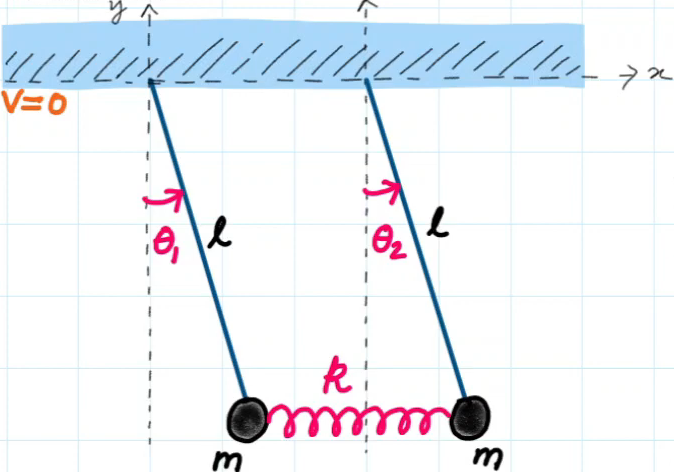
\includegraphics[width=0.98\linewidth]{figs/fig4_cropped_edited.png}
    \caption{Drawn analysis of the simplified coupled pendulum problem [\hyperref[sec:3]{3}]}
\end{figure}
\noindent
the Lagrangian, both $\theta_1$ and $\theta_2$ have similar
form among the terms, and given that $2mg\ell$ is essentially a constant that vanishes from differentiation, 
let $\theta_n$ represent $\theta_1$ then $\theta_2$ when applying the Euler-Lagrange equation for each. Then the process
\begin{gather*}
    \totder[]{t}\parder[\Lagrangian]{\dot{\theta}_n}-\parder[\Lagrangian]{\theta_1}=0 \\
    \left\{\begin{aligned}
        \parder[\Lagrangian]{\theta_n} &= -mg\ell\theta_n \pm k\ell^2(\theta_2-\theta_1) \\
        \totder[]{t}\parder[\Lagrangian]{\dot{\theta}_n} &= m\ell^2\thetaddot_n
    \end{aligned}\right. \\
    m\ell^2\thetaddot_n + mg\ell\theta_n \mp k\ell^2(\theta_2-\theta_1) = 0
\end{gather*}
results in the following system of differential equations
$$\left\{\begin{aligned}
    \thetaddot_1 + \frac{g}{\ell}\theta_1 - \frac{k}{m}(\theta_2-\theta_1) = 0 \\
    \thetaddot_2 + \frac{g}{\ell}\theta_2 + \frac{k}{m}(\theta_2-\theta_1) = 0
\end{aligned}\right.$$
which are second-order, linear, homogeneous, and in standard form.

Solving for either pendulum's equation of motion requires simultaneously solving both of their differential equations as a system of equations.
Futher derivation is reserved for the writing in \textbf{Appendix A} due to the scope of the method of solution becoming more math-focused
(\textit{i.e.}, only the physics portion of the theory behind the simplified pendulums problem is of interest). 
In the end, the equations of motion for the simplified pendulums problem is given as the general solutions
$$\left\{\begin{aligned}
    \theta_1(t) = c_1\cos(\omega_1t) + c_2\cos(\omega_2t) \\
    \theta_2(t) = c_1\cos(\omega_1t) - c_2\cos(\omega_2t)
\end{aligned}\right.$$
for suitable (real) constants $c_1$ and $c_2$ (these are in fact \textit{amplitude} terms).
And according to all assumptions and analogies made in section \textbf{1 Introduction}, these equations of motion also apply to the coupled pendulums experiment in lab
(\textit{i.e.}, the setup shown in \textbf{Figure 1}).

Remarkably, this result implies that predicting the motion of either pendulums only requires the knowledge and the linear combinations of \textit{two} angular frequencies, $\omega_1$ and $\omega_2$,
where $\displaystyle{\omega_1=\sqrt{\frac{g}{\ell}}}$, like in the case of a single simple pendulum, and where different yet similarly $\displaystyle{\omega_2=\sqrt{\frac{g}{\ell}+2\frac{k}{m}}}$
(thus $\omega_2>\omega_1$) [\hyperref[sec:3]{3}].
As intriguing as these definitions are, it is considerably difficult (and uncertain) to determine $k$ from the rubber band in lab,
so these \textit{normal frequencies} $\omega_1$ and $\omega_2$ are left to be experimentally determined,
which typically would also be a difficult task to carry out manually given the system's varying oscillations,
but since data is instead gathered \textit{digitally} via the RMS's attached to each pendulums,
section \textbf{4 Fast Fourier Transform} outlines a robust method to determine these frequencies.


\subsection{Methods}
\subsubsection{Measurements}
Bob masses $m_1$ and $m_2$, where subscripts $_1$ and $_2$ represent the ``left'' and ``right'' pendulums  respectively when viewing the apparatus in \textbf{Figure 1} at the front,
were weighed in as $m_1=75.431\g$ and $m_2=75.496\g$ via an electronic balance.
With a standard ruler measuring in metric (and thus having a precision of 1 mm), the masses were carefully attached 15.5 cm from their centers of mass to the pivot joint made between each respective pendulum shaft and RMS pulley wheel, thus $\ell=$ 0.155 cm.
From these parameters, it is expected that each pendulum's natural frequency $\nu$ be approximately 1.266 Hz in value as calculated given the definition
$$\nu = \frac{1}{2\pi}\sqrt{\frac{g}{\ell}}$$

\subsubsection{Data Collection}
RMS's and software equipments were provided by PASCO scientific, and under the PASCO Capstone software, RMS's were programmed for 1440 divisions per second each,
and sampling rate for data recording was set to 100 Hz (an imperative detail to be mentioned again in section \textbf{4 Fast Fourier Transform}).
The general methodology followed when gathering data was to first start recording when the pendulums were \textit{at rest} before lifting one of the pendulum up to a moderate angle as the initial position.
The amount of oscillations observed after letting go varied depending on the goal of gathering the data, but for all data gathered no less than 5 oscillations were always observed.
All data gathered were exported as \texttt{.csv} files, saving only the time and angular displacement data (PASCO Capstone provides velocity and acceleration data as well, but only the raw data was of interest).
This data was to then be processed and presented via the analysis method outline in section \textbf{5 Data Analysis}.

\subsubsection{Calibration}
Since the theory behind the setup relied on the assumption that the pendulums are \textit{identical} to one another,
data on each individual pendulum \textit{without} coupling was first gathered in order to verify this.
Data on the left pendulum was gathered first before data on the right pendulum was gathered.
Both pendulums were allowed to oscillate 5--6 times before pausing the data recording for exporting.
After experimentally obtaining each both pendulums' individual frequency values (via again the method outlined in section \textbf{5 Data Analysis}),
the right pendulum was adjusted by setting its bob mass closer or further away from its pivot point---
bringing the mass closer to increase its natural frequency and \textit{vice versa} (\textit{i.e.}, the right pendulum was adjusted to match the left pendulum).
These steps were repeated under multiple trials until both pendulums have as close as the same frequency as possible.

\subsubsection{Beats}
Ideally, the tension given by the rubber band should be very loose,
so the RMS's where the pendulums are attached to were horizontally adjusted closer/farther in order to have the tension be such that only the slickness of the rubber band's material clinged onto the shafts.
At the final adjustment, the distance between the pendulums shafts end-to-end was measured to be 8.45 cm.
The rubber band was initially set 9.5 cm away down the pivot joints of the pendulums.
Similar to the previous section, both pendulums were allowed to rest before recording data.
Once data recording began, the left pendulum was raised to a moderate initial position.
Due to the rubber band coupling, lifting the left pendulum also caused the right pendulum to also be raised to some initial position, albeit at a considerablely lower angle.
The use of the PASCO Capstone's graphing feature was used to make sure that both pendulums were held still at their initial positions before letting go.
After letting go and setting the pendulums in motion, the system was allowed to oscillate for a total recording time of at least 30 s and at most 60 s.
Three trials of this procedure was repeated for collecting more data.
For further verification of identical pendulums, the same procedure and number of trials were repeated, 
this time displacing the \textit{right} pendulums rather than the left, with expectation that the same normal frequencies were to be observed no matter which pendulum was chosen to be set in motion.
To gather further data and see the effects that different coupling would have on the system, the rubber band was raised by 0.5 cm to decrease the coupling,
then the overall procedure was repeated, \textit{i.e.}, recording data when the pendulums were at rest, first raising the left pendulum, \textit{etc.},
before lowering the rubber band 1cm down from where it was to gather data on increased coupling.
Overall, beats data on 9cm, 9$\sfrac{1}{2}$ cm, and 10cm coupling was gathered, with three trials of left and right pendulum starting conditions each for symmetry testing. 

\subsubsection{Antisymmetric Mode}
Beat frequencies in the system occurs when each individual pendulums have different magnitudes of initial displacement.
For when the values of these match, the system is set in what is called \textit{symmetric} mode,
when the pendulums are off-set at the same side as each other,
and \textit{antisymmetric} mode, when they are off-set at opposite side of each other.
Testing the antisymmetric mode of the system was chosen over testing the symmetric mode of the system simply due to the former stretching the rubber band more than the latter as being more interesting.
Under ideal and exact initial conditions, the pendulums would transfer no energy to each other and instead oscillate \textit{out of phase} with each other,
\textit{i.e.}, lacking an apparent beat frequency for either pendulum's oscillation data.

After starting data recording when the pendulums were at rest, the left pendulum was pulled back to an initial position while the right pendulum was pulled ahead to its initial position.
The PASCO Capstone's graphing software was heavily utilized to assist in ensuring that the pendulums had the same magnitude in initial displacement before letting go.
The system was recorded for the same range of time period--- between 30--60 s.
Three trials of this procedure was repeated before another three trials of the procedure but off-setting the \textit{right} pendulum towards the back instead and \textit{vice versa} was repeated.


\subsection{Fast Fourier Transform}
\subsubsection{Fourier Transform}
The Fourier transform in essence takes values recorded \textit{w.r.t.} time and transform them to data in the \textit{frequency} domain.
Formally in mathematics, it is given as the improper integral
$$\Fourier\big\{f(t)\big\}(\nu)=\int_{-\infty}^\infty f(t)e^{-2\pi \im\nu t}\diff{t}$$
for a function of time $f(t)$, where $\nu$ is oscillation frequency of units Hz and $\im$ is the imaginary unit.
Note that for other definitions of the transformation, angular frequency $\omega$ of units $\sfrac{\!\radian}{\!\s}$ may be of interest instead, thus
$$\Fourier\big\{f(t)\big\}(\omega)=\int_{-\infty}^\infty f(t)e^{-\im\omega t}\diff{t}$$
is an alternative form that the Fourier transform may take on given $\omega=2\pi\nu$.
This direct change however may affect some definitions of the \textit{inverse} Fourier Transform (which fortunately is not of any interest to this paper, so further deliberation on the definition of the Fourier Transform ends here) [\hyperref[sec:5]{5}].

\subsubsection{Discrete Fourier Transform}
In the lab, data points organized in the form of an array are often dealt with rather than whole functions.
Naturally then, the \textit{integral} definition of Fourier Transform is difficult to apply for these arrays of data.
The \textit{discrete} Fourier transform for an array of data $\vec{y}$ of size $N$ is alternatively given as
$$Y_k = \sum_{n=0}^{N-1}e^{-2\pi\im\frac{kn}{N}}y_n$$
where $k=0,\;1,\;\ldots, N-1$.
Computationally, machines can carry out transformation like these as \textit{matrix-vector} multiplication,
\textit{i.e.}, $\vec{Y}=\mathbf{E}\vec{y}$, where $\mathbf{E}$ is a matrix representing the powers of $e^{-\sfrac{2\pi\im}{N}}$.

\begin{figure}[H]
    \begin{tcolorbox}[ % nearly copied straight from Jupyter's exported file
        breakable, size=fbox, boxrule=1pt, pad at break*=1mm,colback=cellbackground, colframe=cellborder
    ]
        \begin{lstlisting}[language=Python] 
from scipy.fft import fft, fftfreq
import numpy as np
# Number of sample points
N = 600
# sample spacing
T = 1.0 / 800.0
x = np.linspace(0.0, N*T, N, endpoint=False)
y = np.sin(50.0 * 2.0*np.pi*x) + 0.5*np.sin(80.0 * 
(*@$\hookrightarrow$@*) 2.0*np.pi*x)
yf = fft(y)
xf = fftfreq(N, T)[:N//2]
import matplotlib.pyplot as plt
plt.plot(xf, 2.0/N * np.abs(yf[0:N//2]))
plt.grid()
plt.show()
        \end{lstlisting} % interesting so margins do matter in this environment
    \end{tcolorbox}
    \caption{Example code of FFT from the \texttt{scipy} [\hyperref[sec:6]{6}]}
\end{figure}

\subsubsection{The FFT Algorithm}
Matrix-vector multiplication operations are known to have a time complexity of $\mathcal{O}(n^2)$ during computation,
but the discrete Fourier transform is specifically unique for having the property of symmetry within its definition that allows
algorithms to instead emply a \textit{divide-and-conquer} approach to its transformation (\textit{i.e.}, continuous halving for its transformation).
Any code or algorithm that follows this approach achieves a time complexity of $\mathcal{O}(n\log_2(n))$ instead and is aptly named as a \textit{FFT} therefore.

FFT often comes as a native feature for standard oscilloscopes, which is typically used during signal detection for electrical/computer engineers.
It is of this paper's interest though to understand how to employ FFT to any given set of data saved using open-sourced code and resources as an alternative. 
\textbf{Figure 5} demonstrates the remarkable ease of writing an FFT script using Python and an open-sourced library \texttt{scipy}.
This base code is further built upon to create a comprehensive graphical output as to be shown in the next section \textbf{5 Data Analysis}.


\subsection{Data Analysis}
Given data collected from following the procedures outlined in section \textbf{3 Methods}, there are at least \textit{three} important graphs that this paper emphasizes:
\begin{enumerate}
    \item The \textit{raw, overlapping} data to showcase the initial positions set for either one of or both pendulums given the experiment.
    \item \textit{Individual} graphs, which are truncated at the point which oscillations were set in motion.
    \item The \textit{FFT graph} of the data for viewing potentially peaks as likely values of constituent frequencies.
\end{enumerate}
For part (2), the need of \textit{clean, whole} waveforms before performing FFT for part (3) ends up necessitating this step,
and showcasing their individual waveforms would allow an observer to better understand and see any potential \textit{phase} difference
(although code developed for this paper does not calculate this).

\textbf{Appendix B} shows nearly all code develop for the analysis outlined.
The code additionally employs a method for finding an approximated point to truncate the raw data,
albeit not perfectly--- the user can adjust this value as an optional paramater however.
For any further interest in this method, 
a discrete convolution was performed on the data set with the given kernel [0, -1, 1] before gathering the maximum value of the transformed array.

While the code does not perform any peak analysis for a given FFT graph,
the application at least returns table views of each signal sorted from highest to lowest value along with its frequency pair.


\subsection{Results and Discussion}
The full analysis report across all data gathered for the many modes, \textit{i.e.}, calibration, beats for three different coupling, antisymmetric mode, and non-identical pendulums,
can be found under \textbf{Appendix C: Full FFT analysis across all data}.
Select outputs included in this paper were chosen for having the most significance in discussing results over the other outputs---
including all graphical outputs in this paper is considered difficult, for each individual analysis results are quite large in figure size and are too enumerous to properly include with writing.

\subsubsection{Calibration Results}
\textbf{Figure 6} reports the analysis done on the left pendulum of the apparatus.
As determined in section \textit{3.1 Measurements}, the expected frequency value to be determined from the peak of the FFT graph was 1.266 Hz.

Trial 2 differed much from trial 1 for:
(1) having greater initial displacement of $0.6\radian$ over $0.5\radian$ as done for trial 1;
and (2) recording $5\sfrac{1}{2}$ oscillations rather than 5 as outlined by the procedure in section \textit{3.3 Calibration}.
Surprisingly, however, these changes brought the peak frequency of the FFT graph closer to the calculated value, with approximately $0.86\%$ error.
The results of these two trials signifies two major ideas:
(1) The FFT accurately reports constituent frequencies \textit{given enough observed waveforms};
and (2) while trial 1's peak frequency value is off from the expected value,
the result from trial 2 is enough to conclude that this is likely due to a lack of sufficient waveforms recorded.

Data gathered from the right pendulum were analyzed like with the left pendulum trials (the graphical report can again be found in \textbf{Appendix C}).
Approximately 5 oscillations were recorded for the two trials, so there is unfortunately no left-pendulum ``trial 2'' to verify if both left and right pendulums are identical.
therefore this paper turns to a common statistics test to determine instead if the pendulum frequencies are \textit{statistically} significant from one another.

The mean and standard deviation from the frequency peaks determined by the FFT analysis on the right pendulum is calculated as $1.147\pm0.022\Hz$.
A third trial was additionally ran for the left pendulum, returning a frequency peak of approximately 1.141 Hz for 5 oscillations.
Then for a FFT of 5 oscillations, the left pendulum has a natural frequency
\end{multicols}
\newpage
% \begin{onecolumn}
\begin{figure}[H]
    \centering
    \begin{subfigure}{0.49\linewidth}
        \centering
        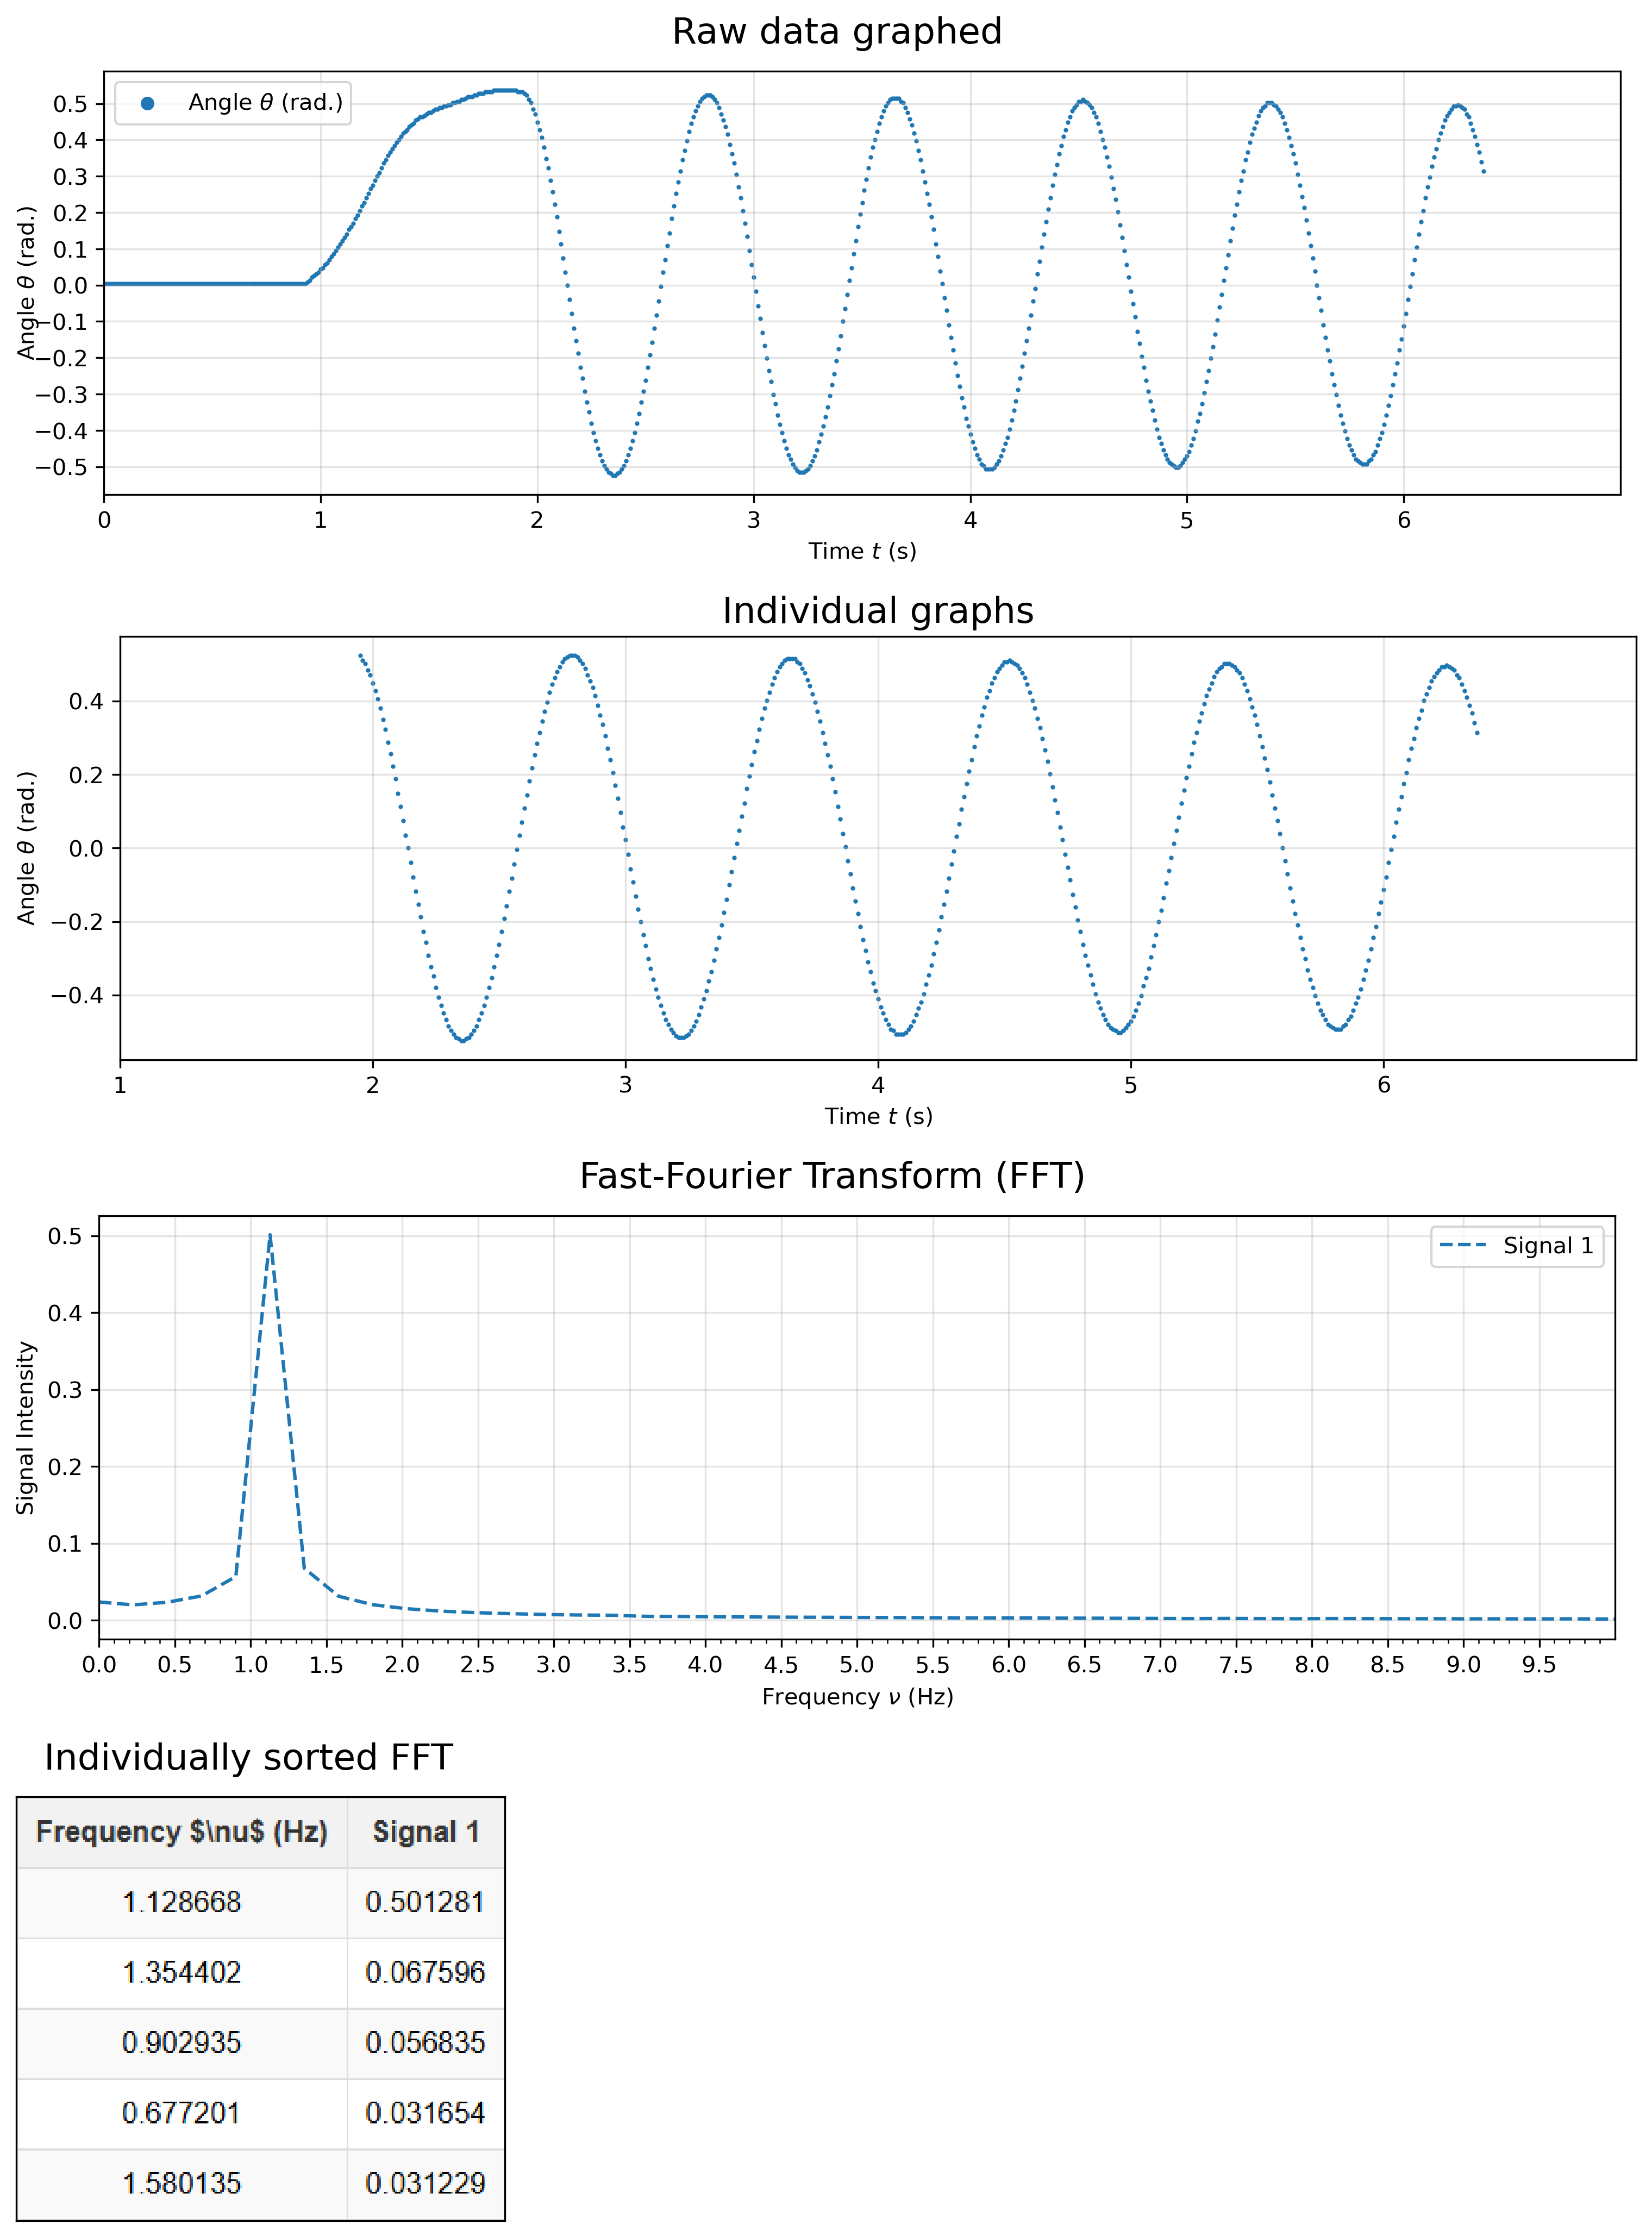
\includegraphics[width=0.98\linewidth]{figs/left pendulum trial 1.png}
        \caption{Trial 1 of gathering left-pendulum oscillation data}
    \end{subfigure}
    \begin{subfigure}{0.49\linewidth}
        \centering
        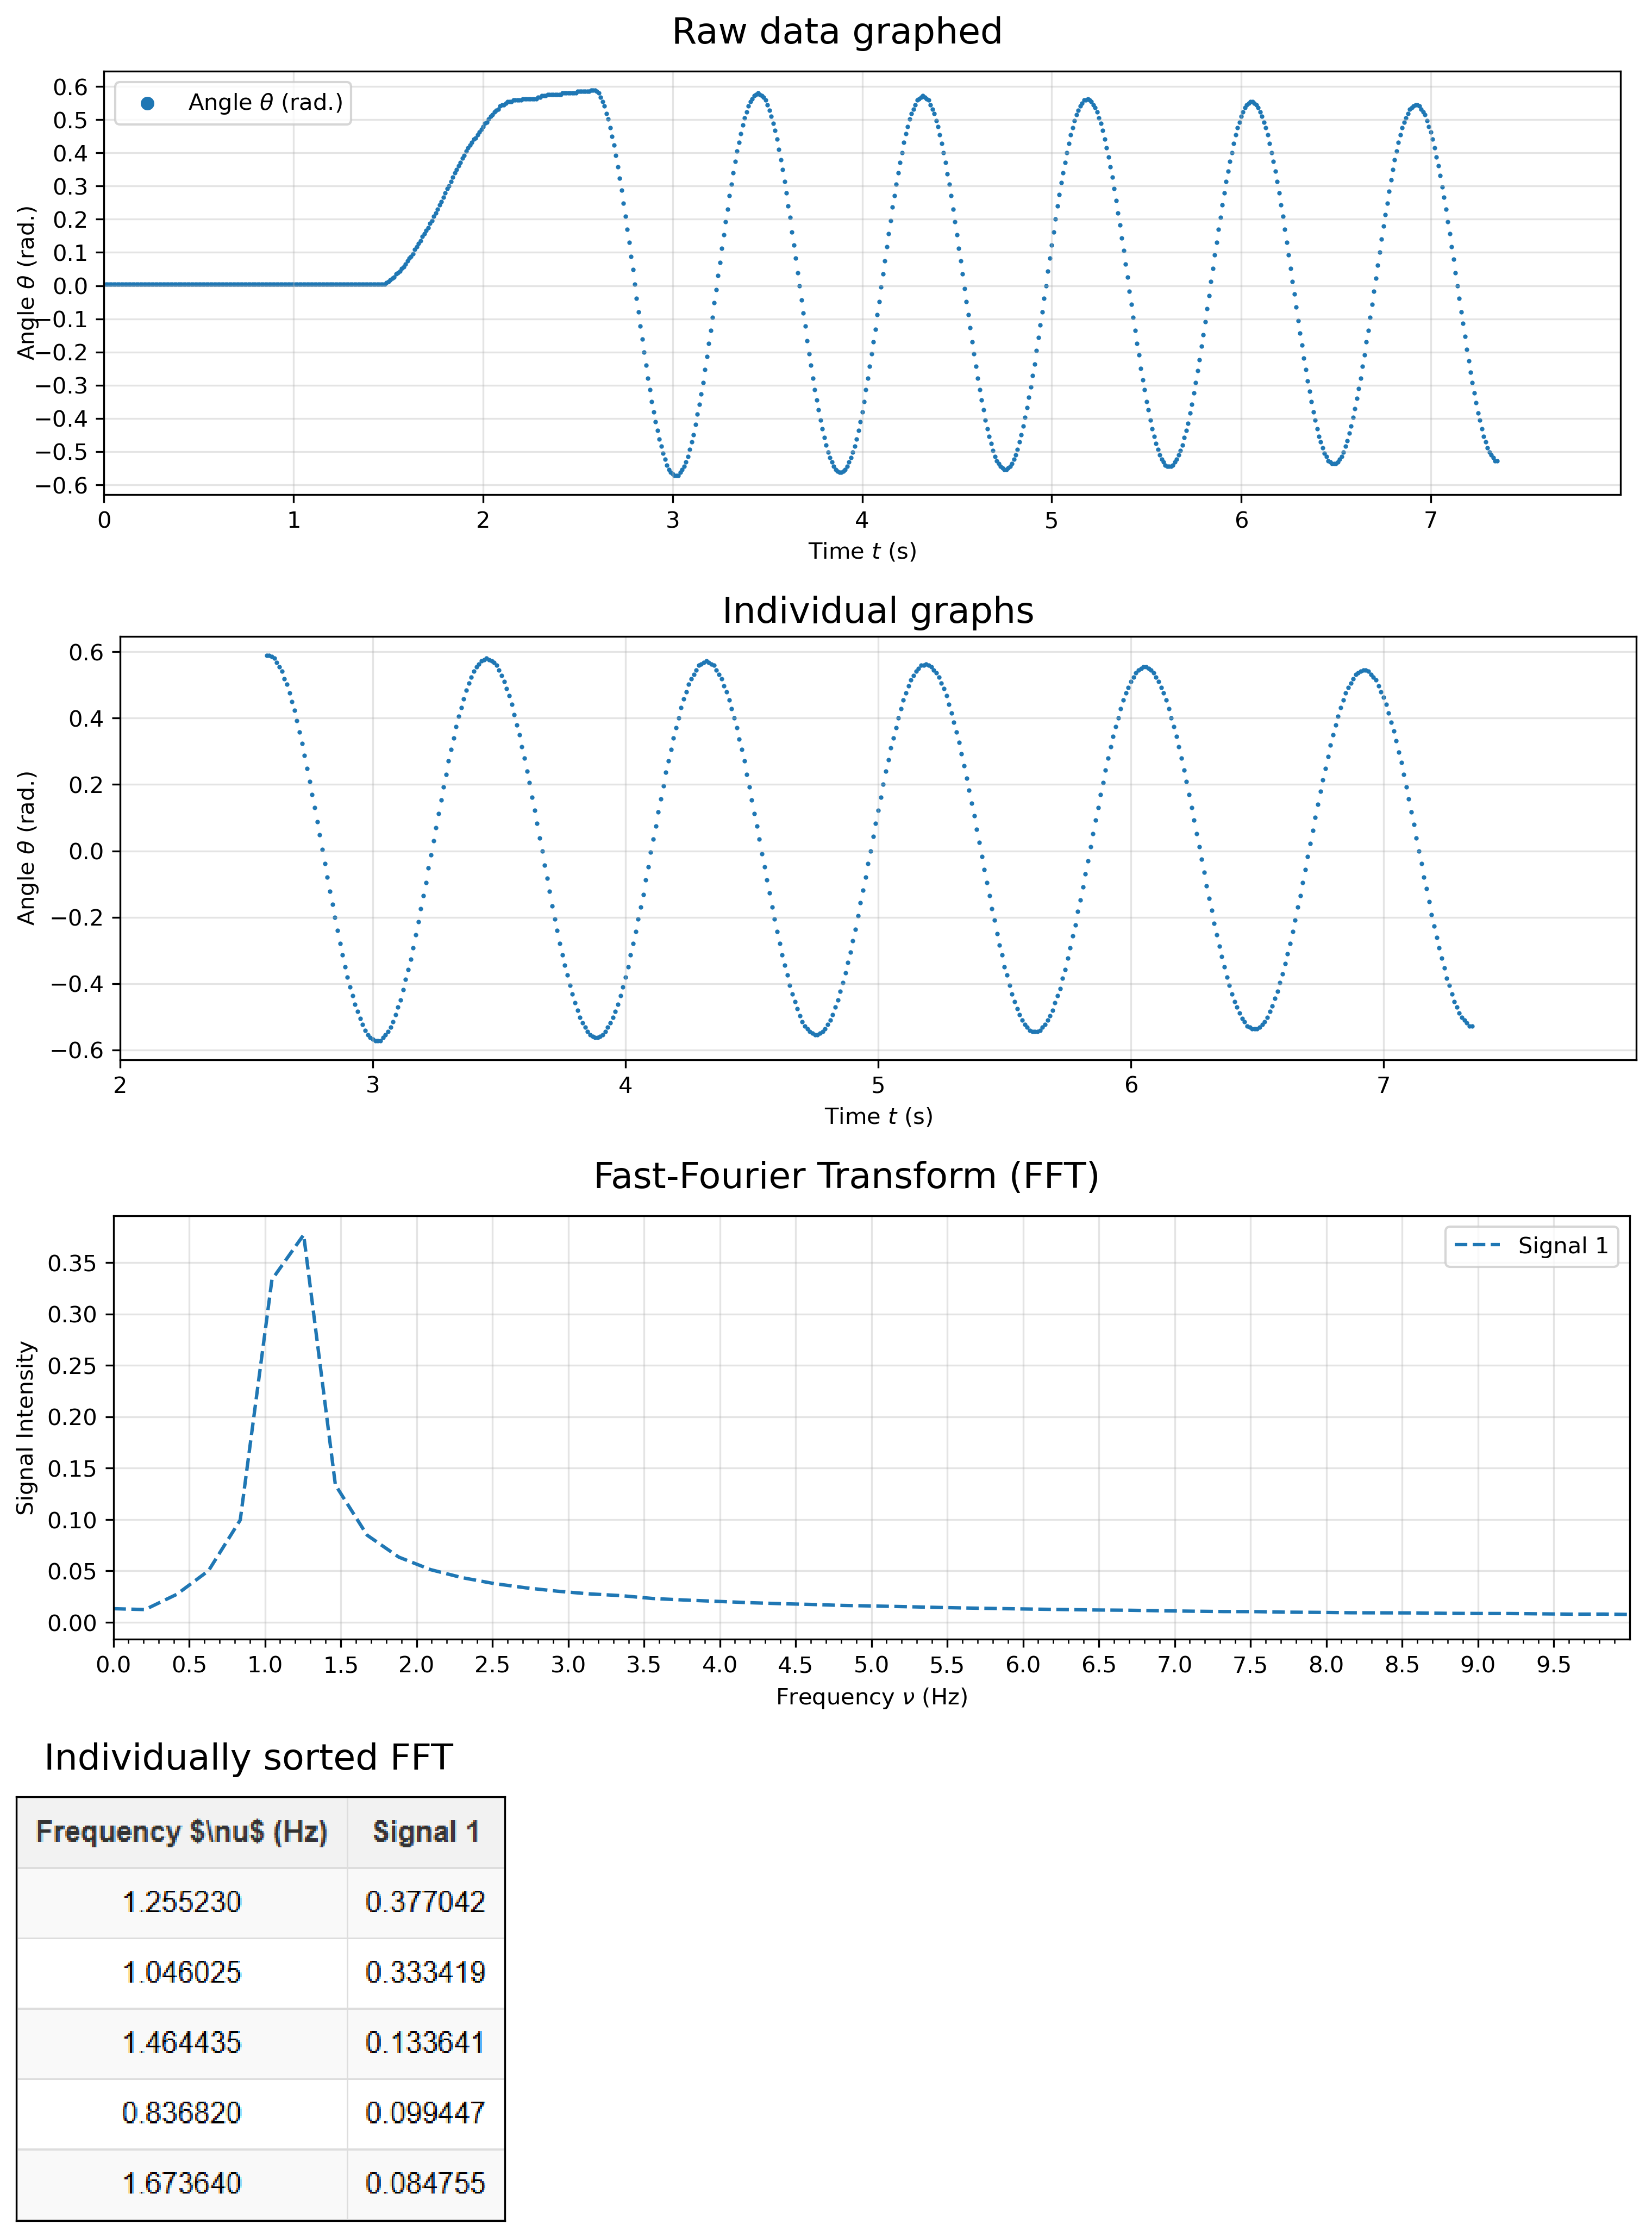
\includegraphics[width=0.98\linewidth]{figs/left pendulum trial 2.png}
        \caption{Trial 2 of gathering left-pendulum oscillation data}
    \end{subfigure}
    \caption{Full analysis on the natural oscillations of the left pendulum of the apparatus}
\end{figure}
% \end{onecolumn}
\begin{multicols}{2}
\noindent
of $1.135\pm0.009\Hz$.
Running a T-statistics test on these parameters returns a $p$-value of approximately 0.587. 

In statistics, normally a $p$-value $<0.05$ is sought after, 
for it is conclusive evidence that two datasets are statistically significant, or \textit{different}, from one another,
but since the goal of this analysis is to prove that the pendulums are \textit{identical} to one another,
the ``insignificant'' results from having such a high $p$-value works in favor in showing the similarity of the two pendulums.
Consider treating the results of trial 2 of the left pendulum as validation for the measurements of the left pendulum and using the test statistics as proof of similarity.
Then overall the pendulums can indeed be said to be identical.
\vfill

\subsubsection{Beats Results}
Overall, there are 17 analysis reports for the beats mode (one data set was incorrectly saved, which was trial 3 of left-pendulum starting condition with 9$\sfrac{1}{2}$ cm coupling).
According to the equations of motion obtained from section \textit{2.3 Euler-Lagrange Equations},
there should two frequencies which should emerge as dominant peak values on an FFT graph, and furthermore such FFT graphs from both pendulum should nearly be identical.
From an overview on all individual waveform graphs across all data, and because the equations of motion differ by a sign, 
it is strongly believed that both pendulums have the same waveform, just out of phase with each other by $\pi$. 
\textbf{Figure 7} shows the best analysis reports made for the 9 cm, 9$\sfrac{1}{2}$ cm, and 10 cm coupling trials each according to
\end{multicols}
\newpage
\begin{figure}[H] % half of the figure
    \centering
    \begin{subfigure}{0.49\linewidth}
        \centering
        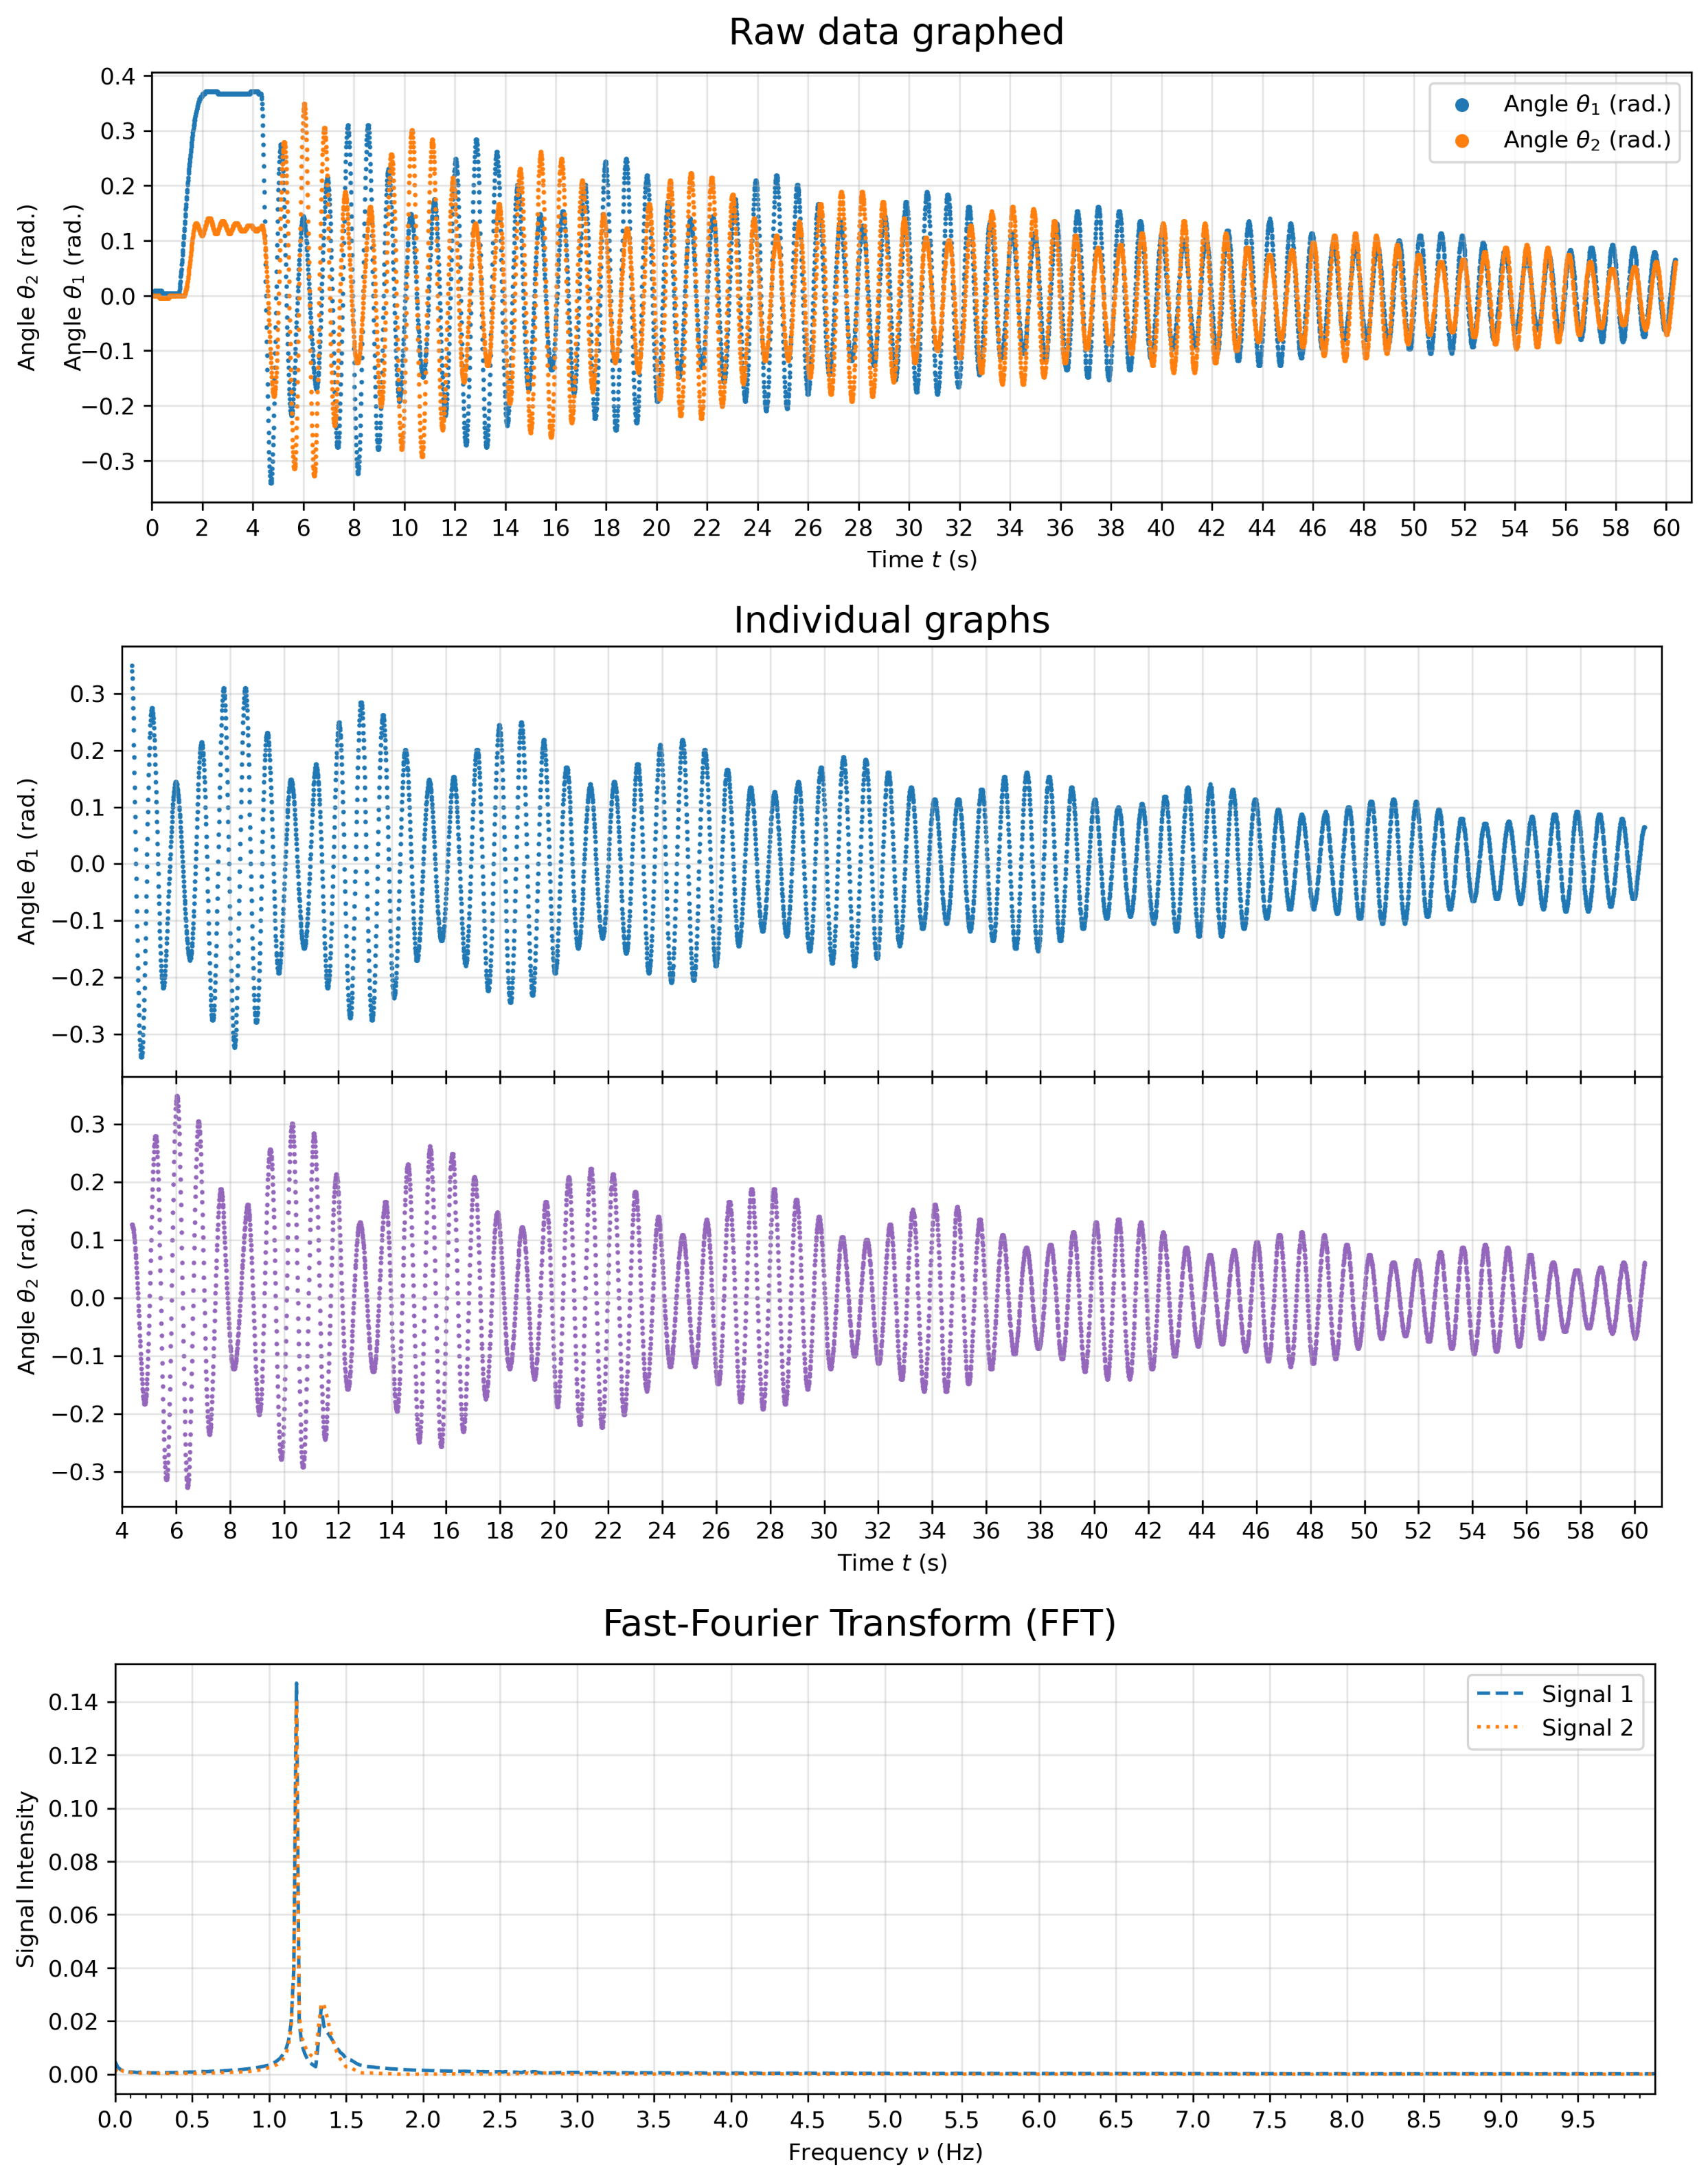
\includegraphics[width=0.98\linewidth]{figs/beat (left_9_3)_cropped.png}
        \caption{Clearest FFT graph for 9 cm coupliing}
    \end{subfigure}
    \begin{subfigure}{0.49\linewidth}
        \centering
        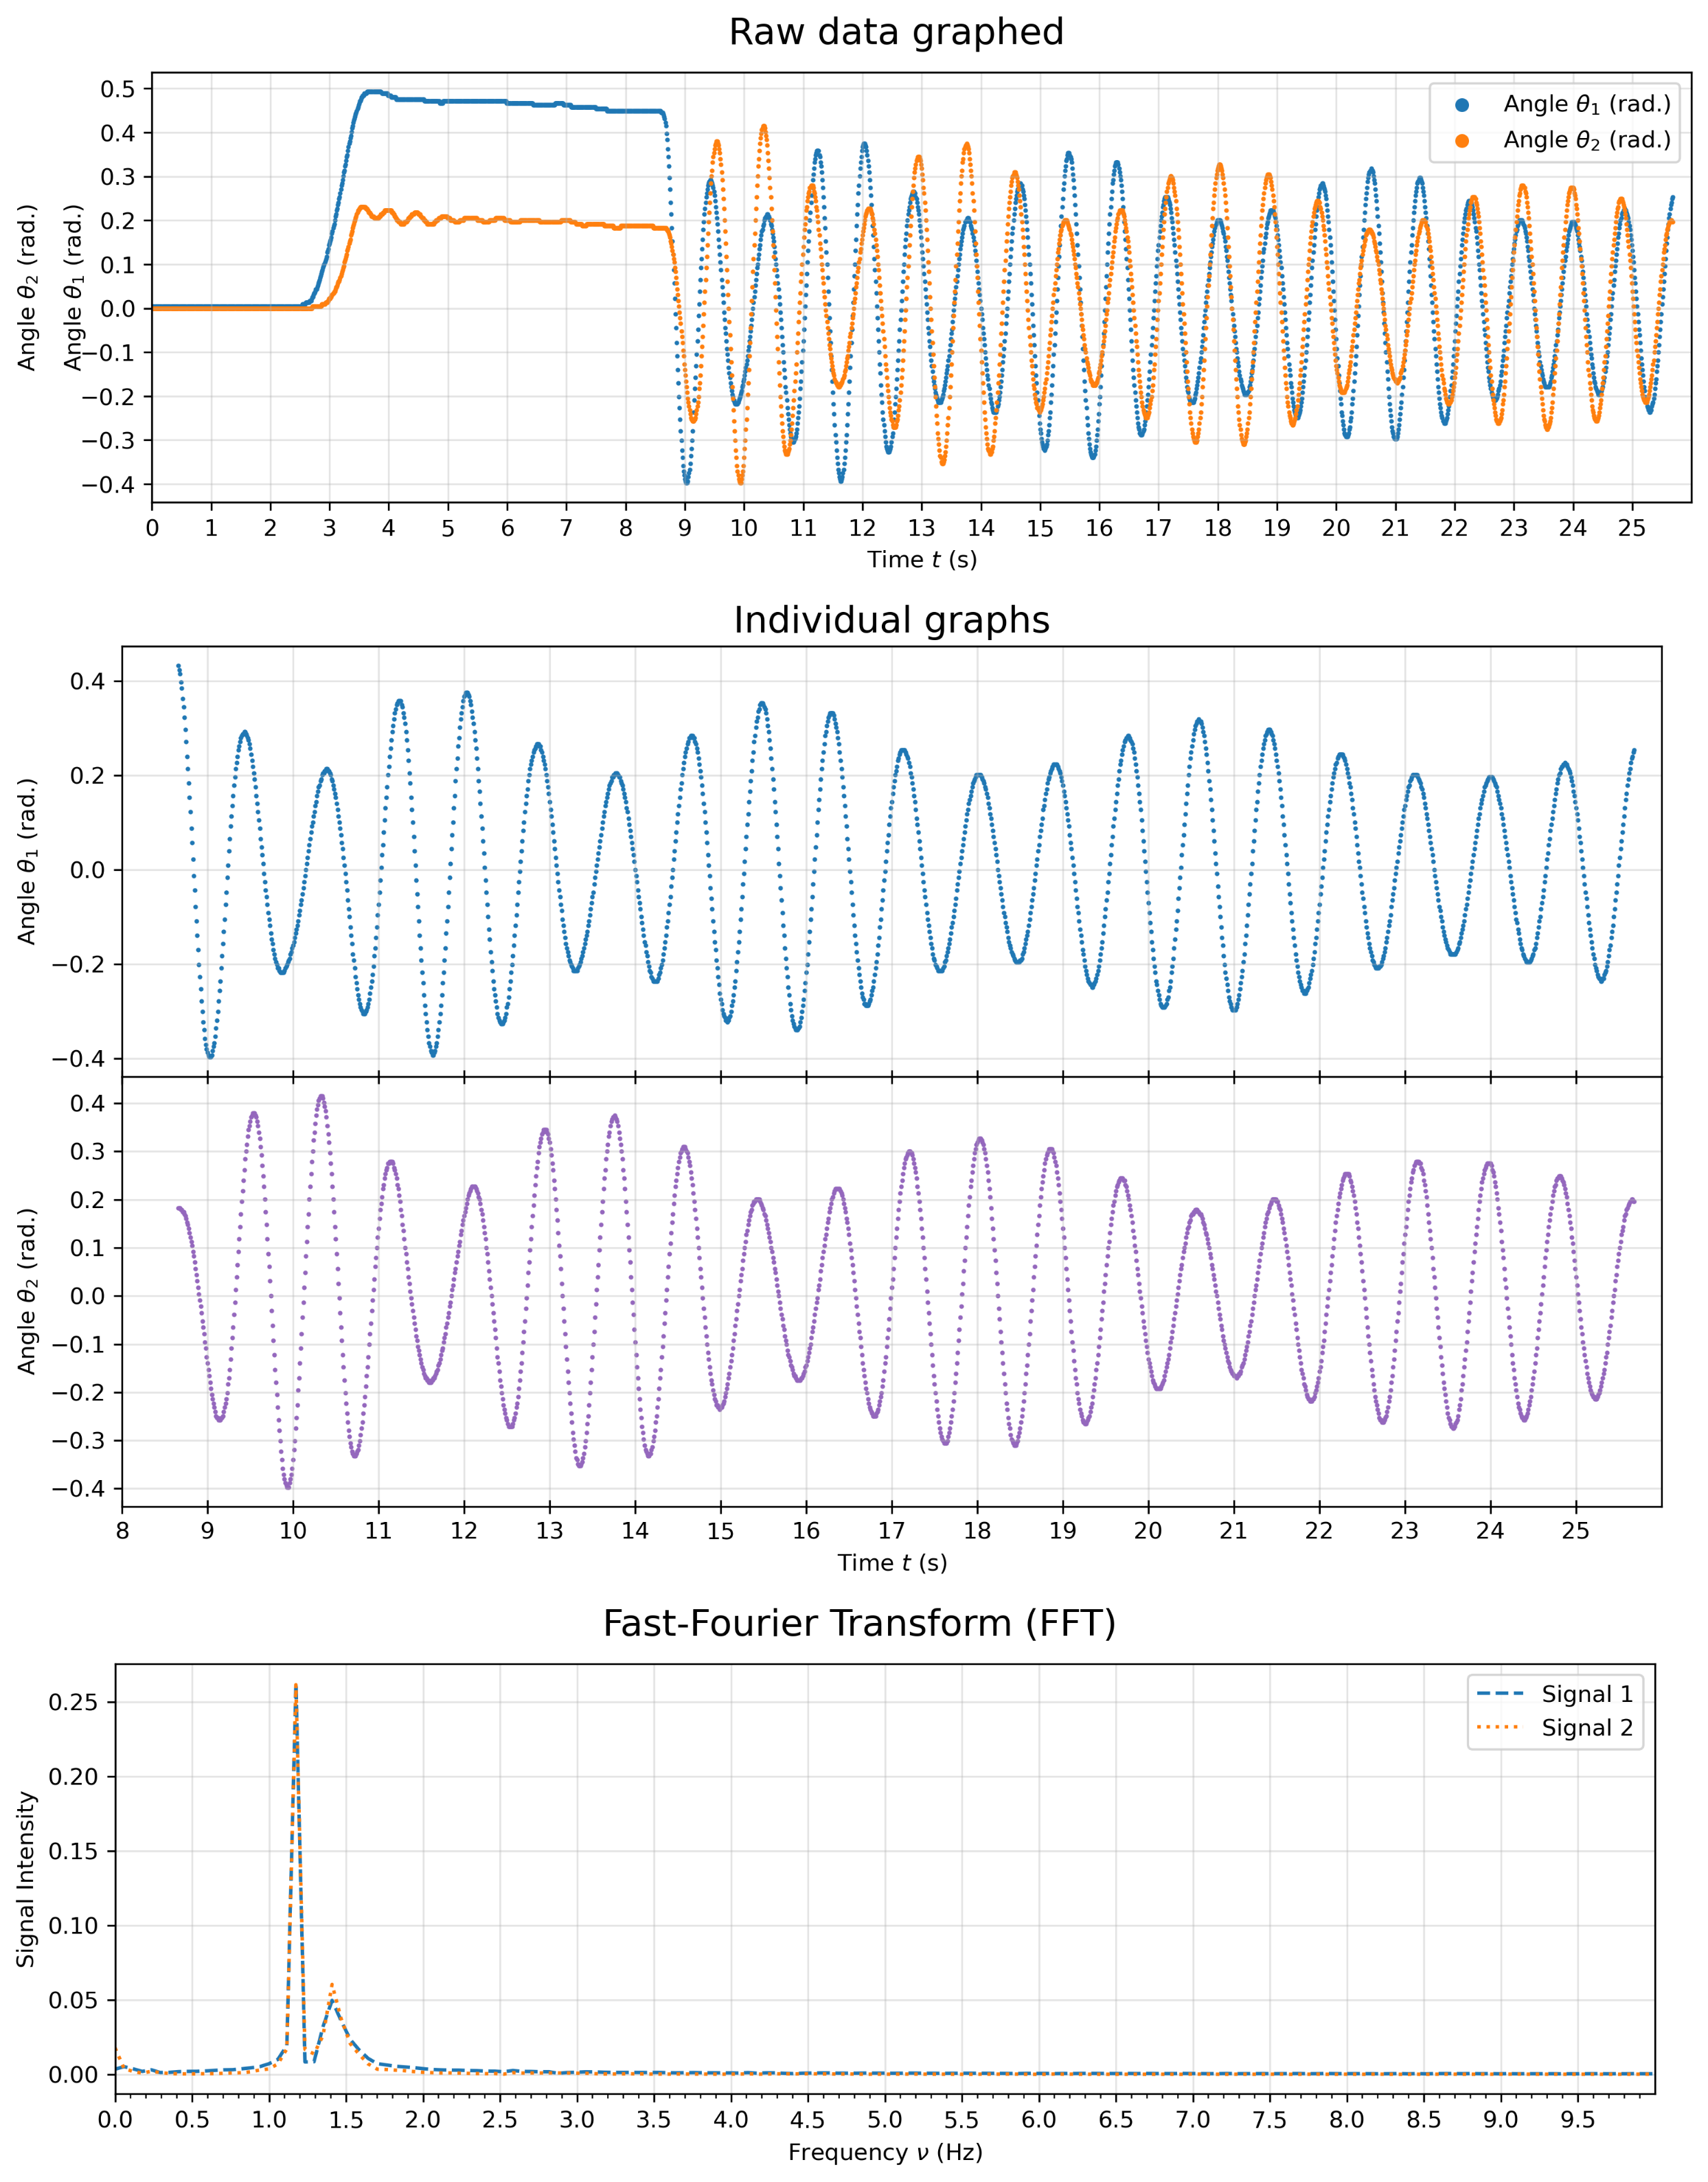
\includegraphics[width=0.98\linewidth]{figs/beat (left_9-5_1)_cropped.png}
        \caption{Clearest FFT graph for 9$\sfrac{1}{2}$ cm coupliing}
    \end{subfigure}
    \caption{Best FFT analysis reports for 9 cm, 9$\sfrac{1}{2}$ cm, and 10 cm coupling settings}
\end{figure}
\begin{multicols}{2}
\noindent
their FFT graphs.
These were chosen out of the 17 analysis report for having the most identical FFT graphs from either pendulums given the trial run.

Although it is not shown in \textbf{Figure 7} (for formatting reasons),
the \textbf{Individually sorted FFT} table strangely does not return the peak values as the top two pair---
rather, some intermediary frequency value gets reported,
and thus while what is extremely likely to be $\omega_1$ gets reported as the strongest value always,
the frequency that is most likely to be $\omega_2$ would be the third or even fourth highest value if its not reported as the second.
Regardless, it can be observed in \textbf{Figure 7} that the beat frequencies for each pendulum are indeed out of phase with each other---
this is most easily seen in the \textbf{Raw data graphed} portion of the analysis reports.
After manual review of the \textbf{Individually sorted FFT} tables,
the highest peak frequencies reported for the ideal 9 cm, 9$\sfrac{1}{2}$ cm, and 10 cm coupling trials are 1.178151 Hz, 1.174398 Hz, 1.176737 Hz, respectively---
these values each also show up as the top values for both signals given the trial.
As these values likely represent $\omega_1$, and beceause $\displaystyle{\omega_1=\sqrt{\frac{g}{\ell}}}$, it is expected that they would be nearly identical in values.
It can be said then that $\omega_1$ for the beat pendulums trials $7.39172\pm0.01191$ $\sfrac{\radian}{\s}$.
However, as consistent as these values are, what is not consider consistent is the comparison of the values to the theoretical value of 1.266 Hz,
which has a 7.075\% error to the theoretical.
It is currently not understood why the values are different rather than exact.

Any reader attempting to find the second frequency peak should compare the other values on \textbf{Individually sorted FFT} tables with what is shown on the \textbf{Fast-Fourier Transform} graph to find the
\newpage
\begin{figure}[H]
    \centering
    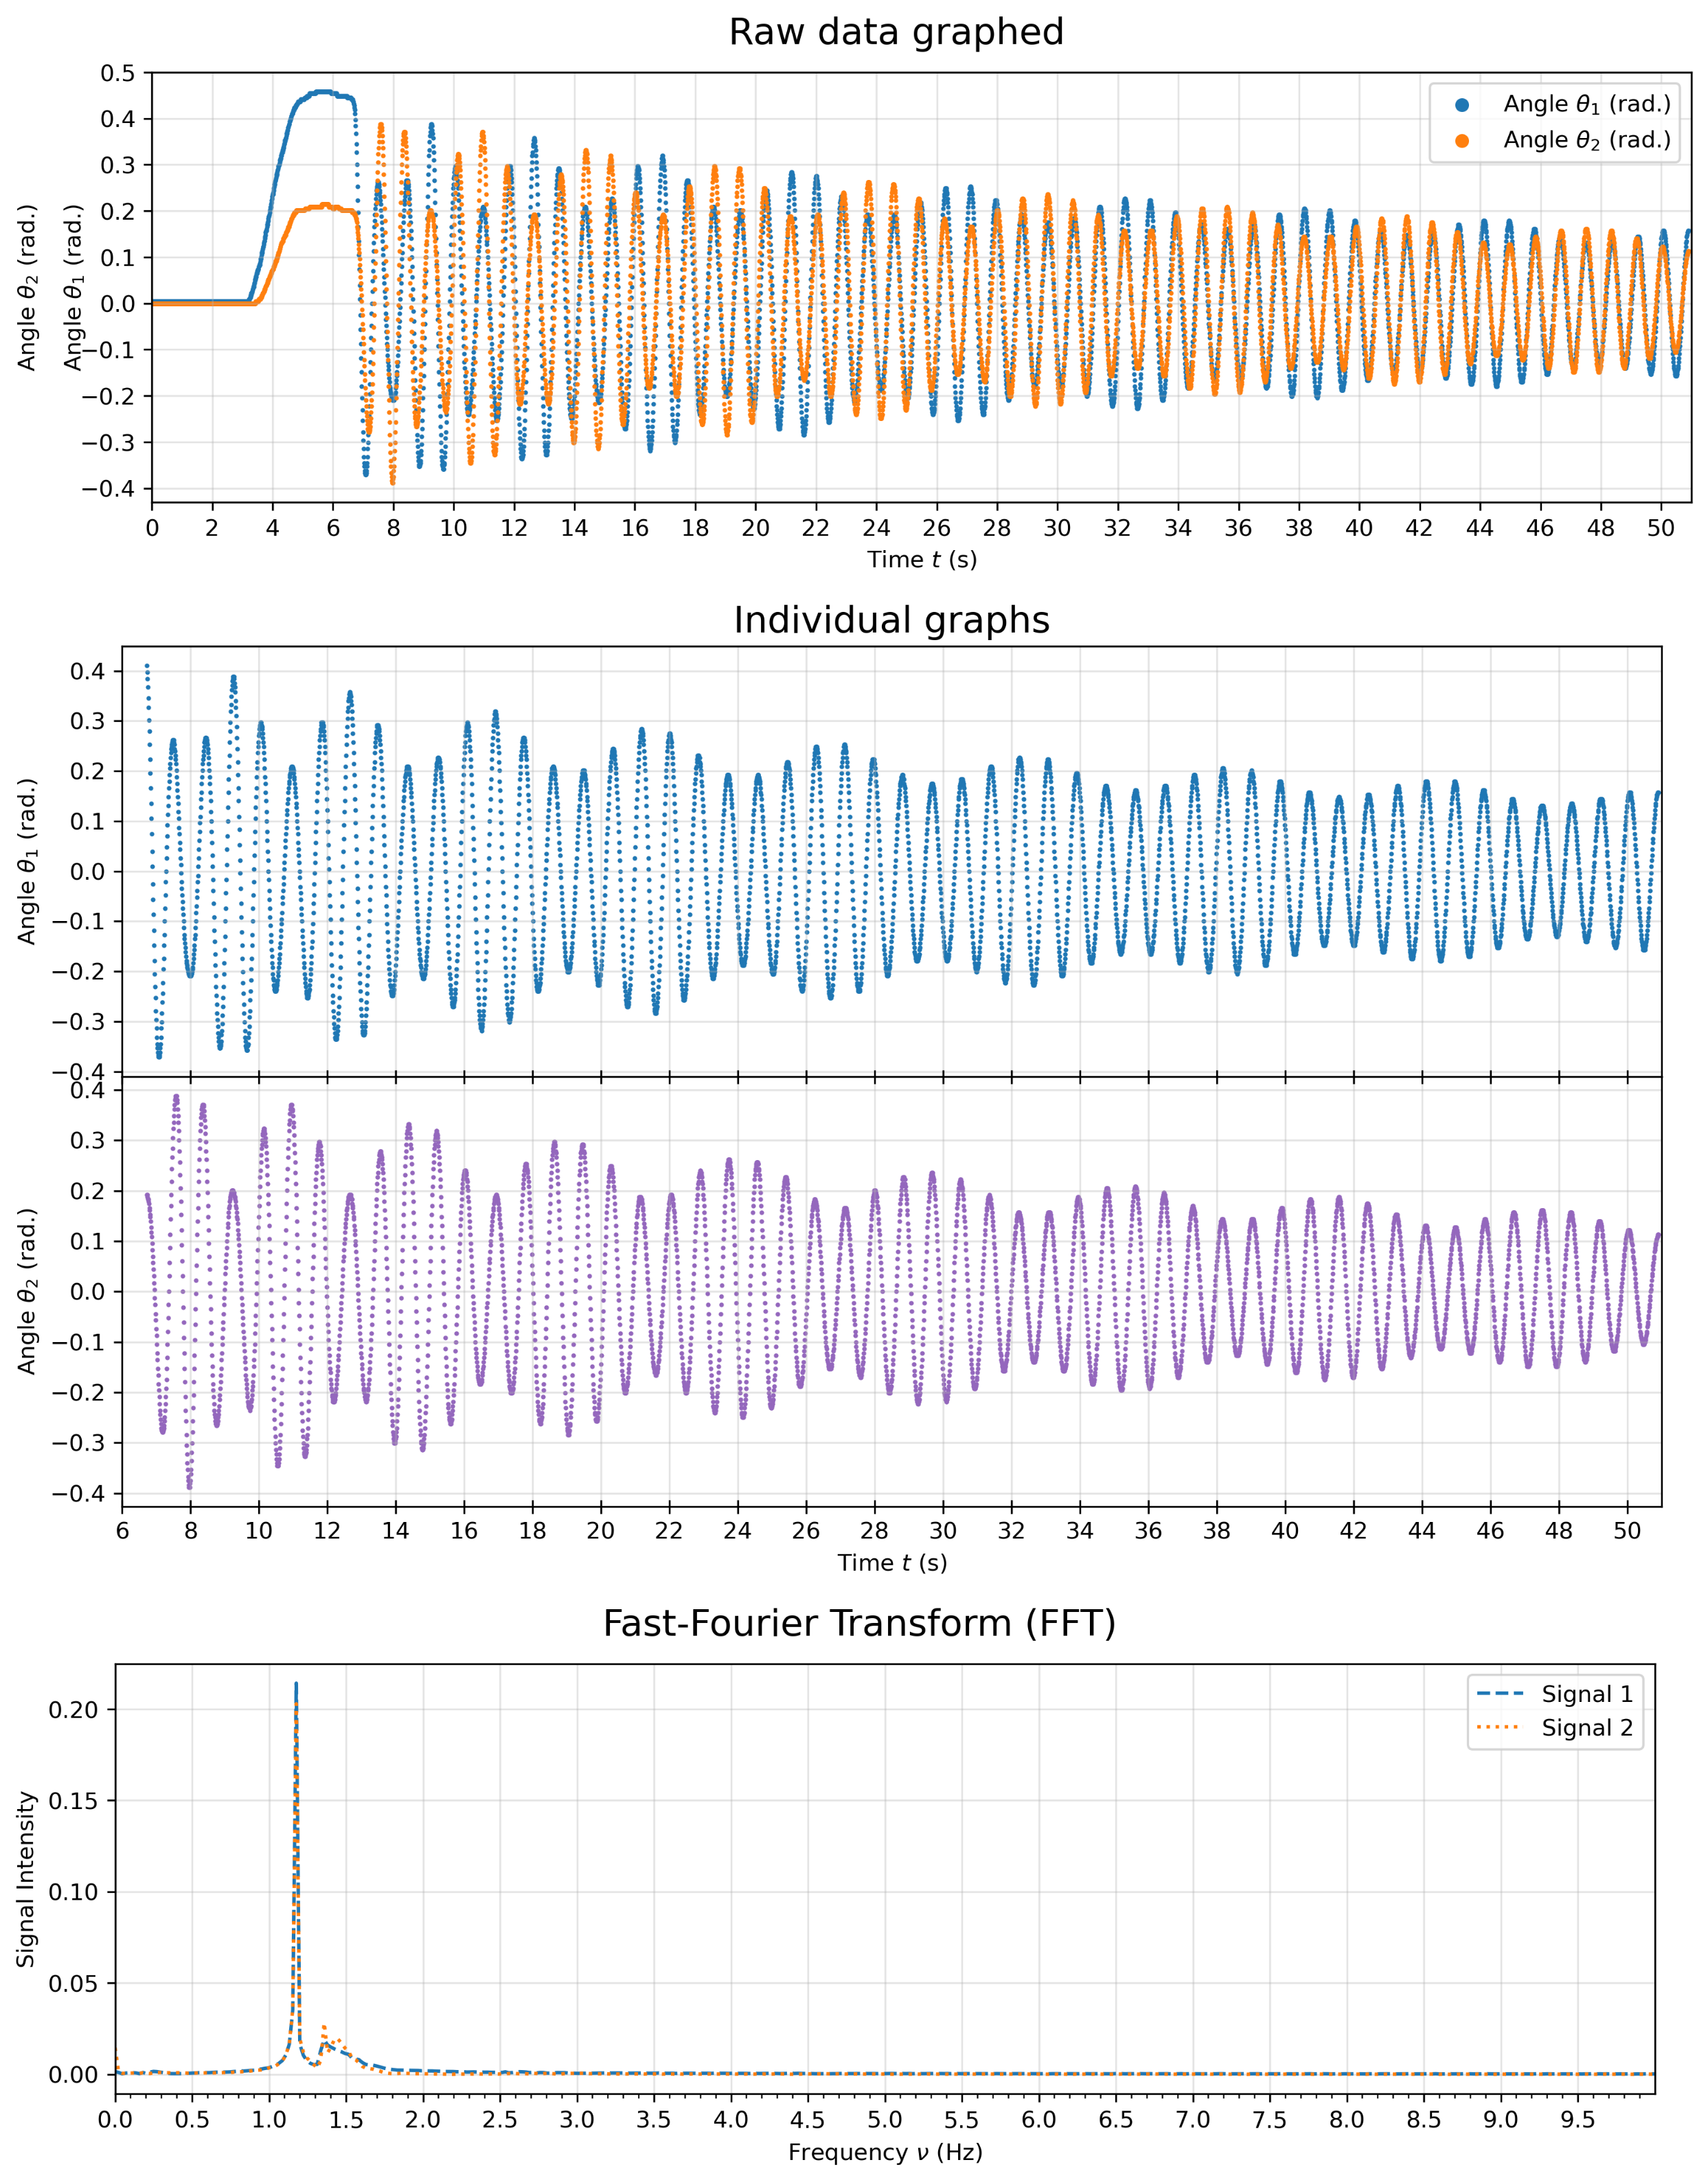
\includegraphics[width=0.98\linewidth]{figs/beat (left_10_2)_cropped.png}   
    \captionsetup{labelformat=empty}
    \caption{(c) Clearest FFT graph for 10 cm coupliing}
\end{figure}
\noindent
appropriate values.
This paper identifies 1.338808 Hz, 1.409278 Hz, and 1.357773 Hz as the second peak values for the ideal 9 cm, 9$\sfrac{1}{2}$ cm, and 10 cm coupling trials.
Each coupling then has an $\omega_2$ value 8.412 $\sfrac{\radian}{\s}$, 8.855 $\sfrac{\radian}{\s}$, and 8.531 $\sfrac{\radian}{\s}$ for the same respective coupling settings.
It is expected that $\omega_2$ changes in value for different couplings, for the value of $k$ representing the elasticity (or ``spring'' as it was modelled after in the simplified pendulums problem) constant changes depending on the position of the rubberband.
What is also strange for these values is that the change in $\omega_2$ values does not proportionally change with coupling strength, \textit{i.e.}, $\omega_2\; \cancel{\propto}\; k$.
The 9$\sfrac{1}{2}$ cm coupling has the highest $\omega_2$ value.
A final note before closing of this section is the abnormality in the second peak for the best 10 cm coupling FFT graph---
despite this analysis report being chosen as the best FFT graph, signal 1 in the FFT graph has some bumps in its peak for $\omega_2$ when compared to signal 1.

\subsubsection{Antisymmetric Mode Results}
\textbf{Figure 8} shows two FFT analysis reports out of the six trials--- 3 trials where the left pendulum was set back and 3 trials \textit{vice versa}---
where the  \textbf{8a} and \textbf{8b} are when the left pendulum was swung back and right pendulum was swung back, respectively.
It can be seen that an observer when gathering data adjusted the pendulum starting conditions based on the live data feed from PASCO Capstone---
a starting condition of 0.3 $\radian$ for both pendulums can be seen chosen then.
The goal of this figure is to show a non-ideal trial for the antisymmetric mode and a more ideal one.
As discussed in section \textit{3.5 Antisymmetric Mode}, there should ideally be no beat frequency to be identified in the graphs, for the rubber band coupling no longer allow energy transfer between the pendulums.
\textbf{8a} shows a clear beat frequency, and thus its inclusion in this paper act as indication for an unsuccessful antisymmetric mode trial run.
On the other hand, \textbf{8b} shows a more ideal trial run, where the beat frequency is visible more surpressed as compared to \textbf{8a}, albeit not entirely undetectable.
The \textbf{Fast-Fourier Transform (FFT)} graphs for \textbf{8a} and \textbf{8b} hint at what the ideal FFT graph for a properly ran antisymmetric mode trial should look like.
For \textbf{8a}'s FFT graph, it resembles the two-peak graph pattern that is prevalent amongst the graphs in \textbf{Figure 7}.
However, \textbf{8b}'s FFT graph seems to show a convergence of all smaller peaks that an unsuccessful antisymmetric mode run would result into a single, uniform peak.
But given that the best antisymmetric mode run is not as ideal as it could be, the dominant frequency $\omega$ from an antisymmetric mode result is inconclusively reported.
\vfill

\end{multicols}
\newpage
\begin{figure}[H]
    \centering
    \begin{subfigure}{0.49\linewidth}
        \centering
        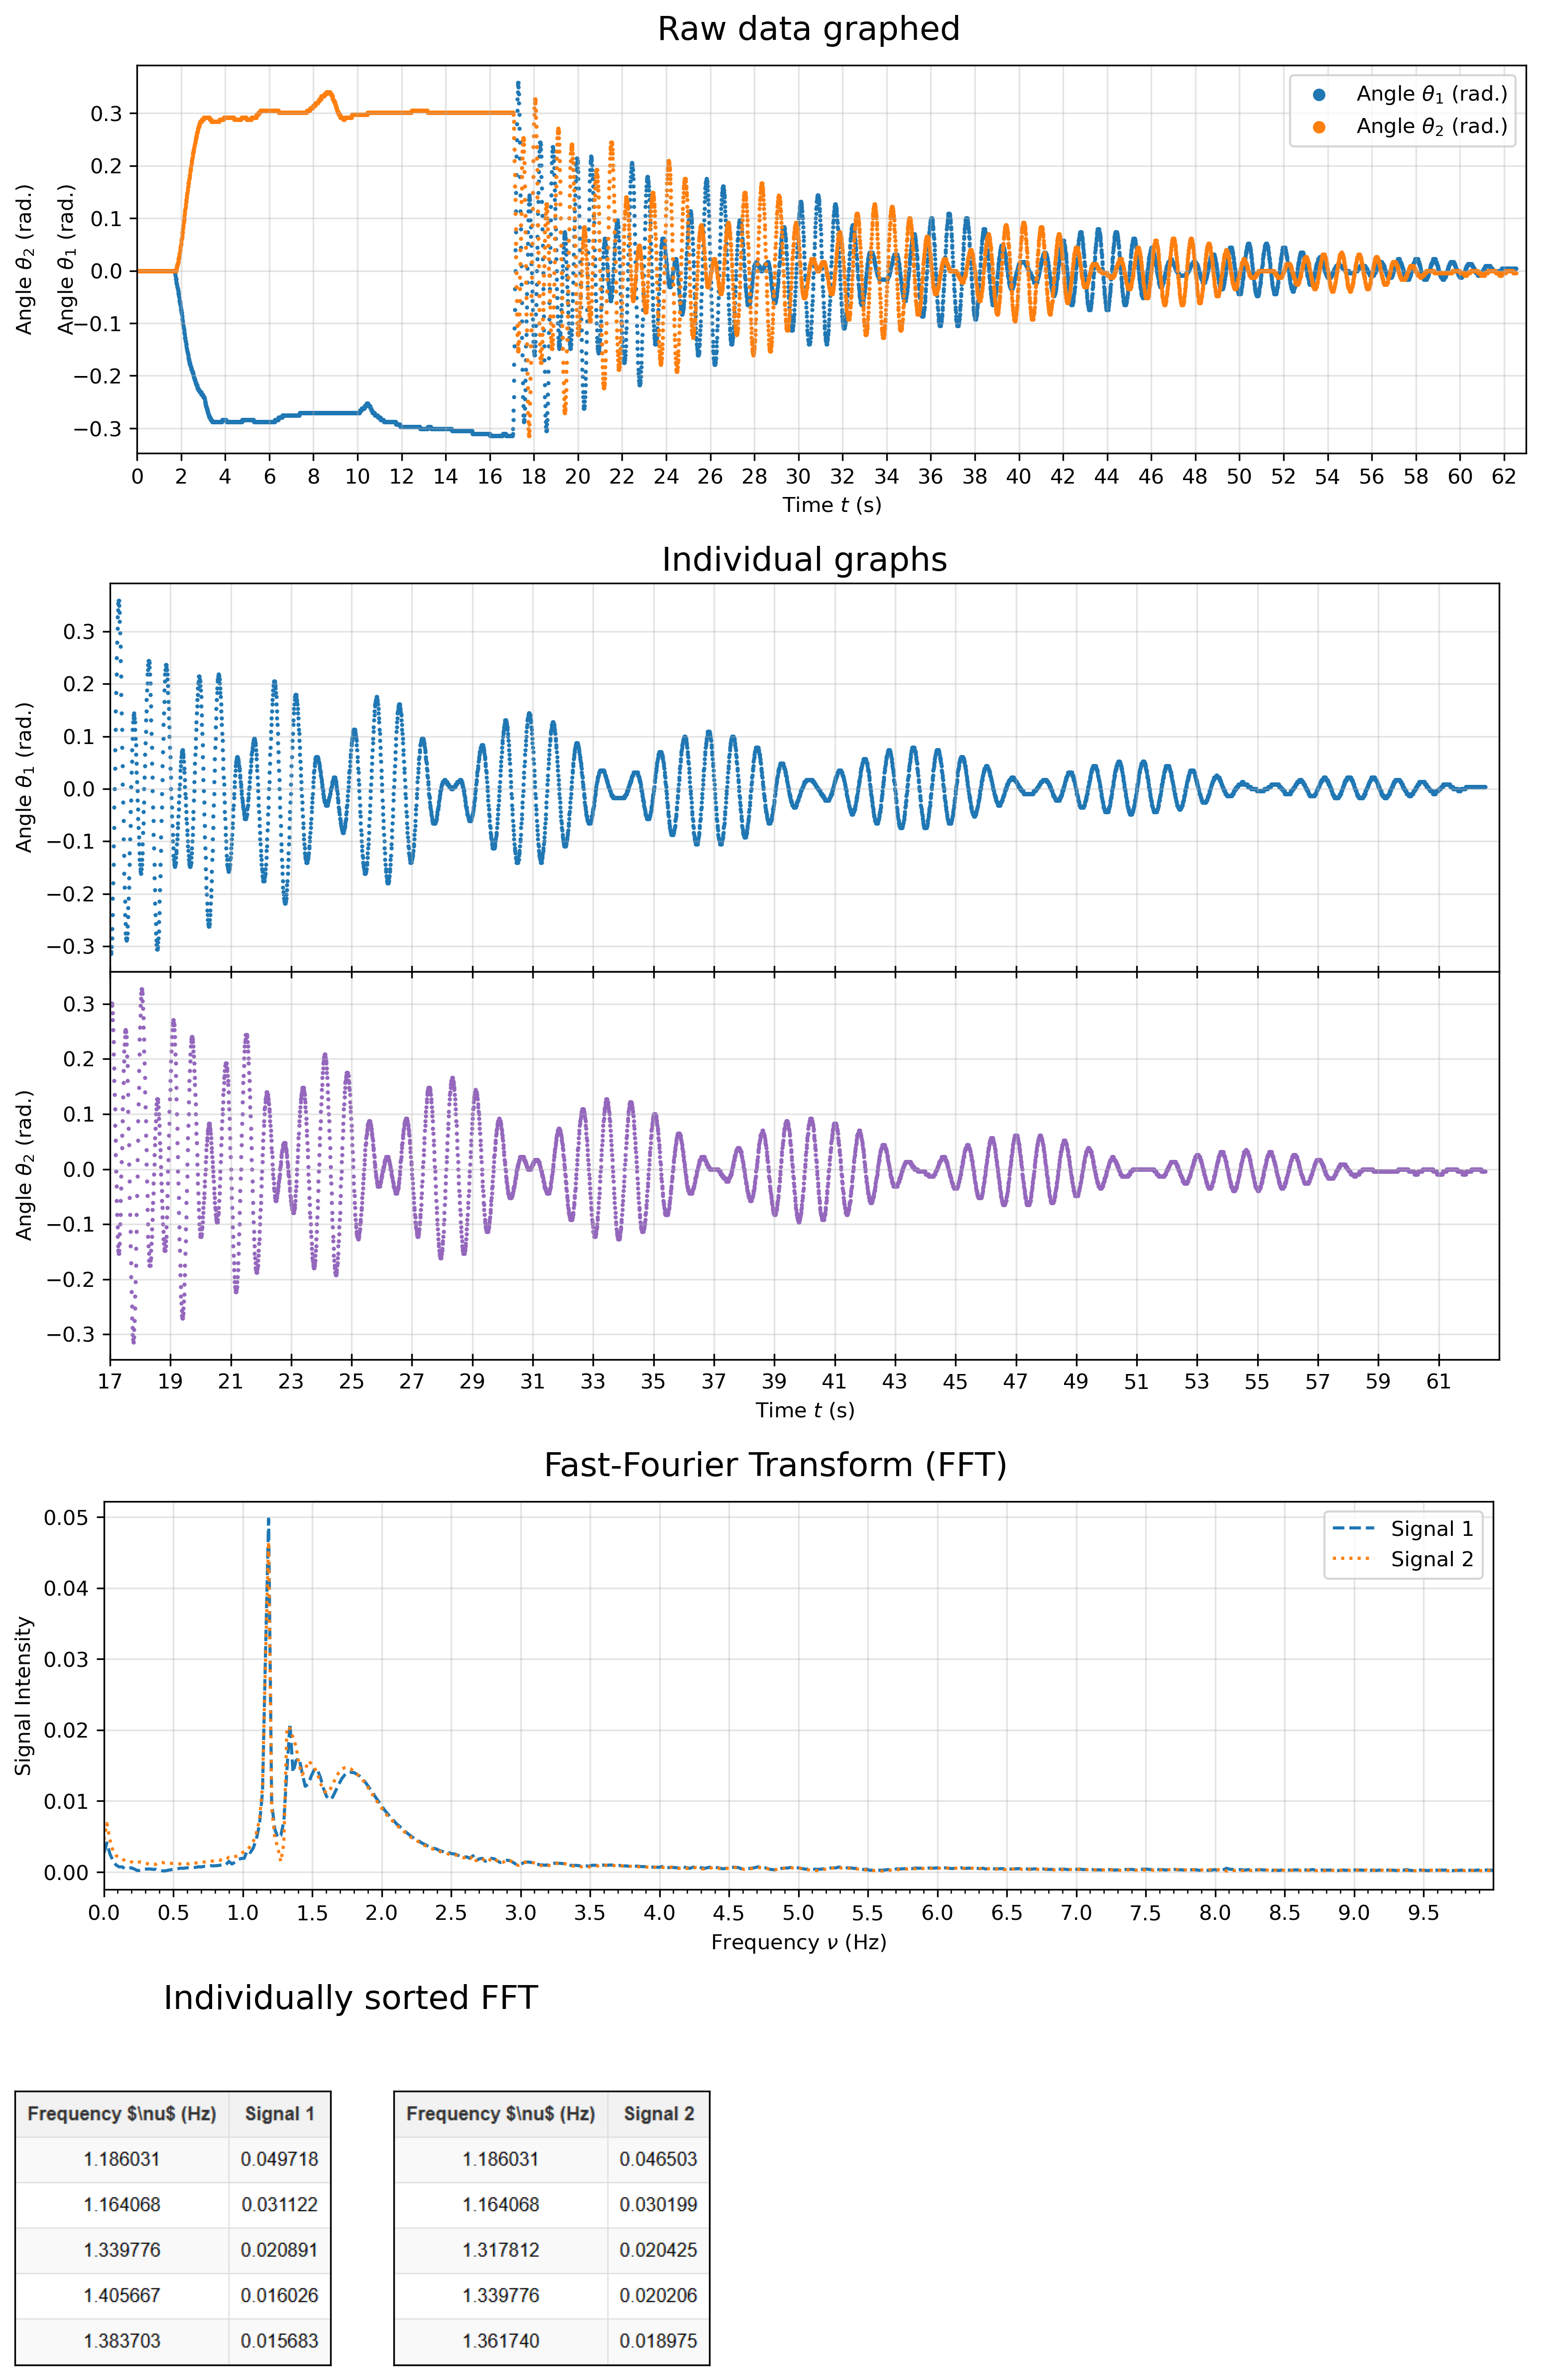
\includegraphics[width=0.98\linewidth]{figs/anti pendulum (left-back_1).png}
        \caption{First trial done for the antisymmetric mode}
    \end{subfigure}
    \begin{subfigure}{0.49\linewidth}
        \centering
        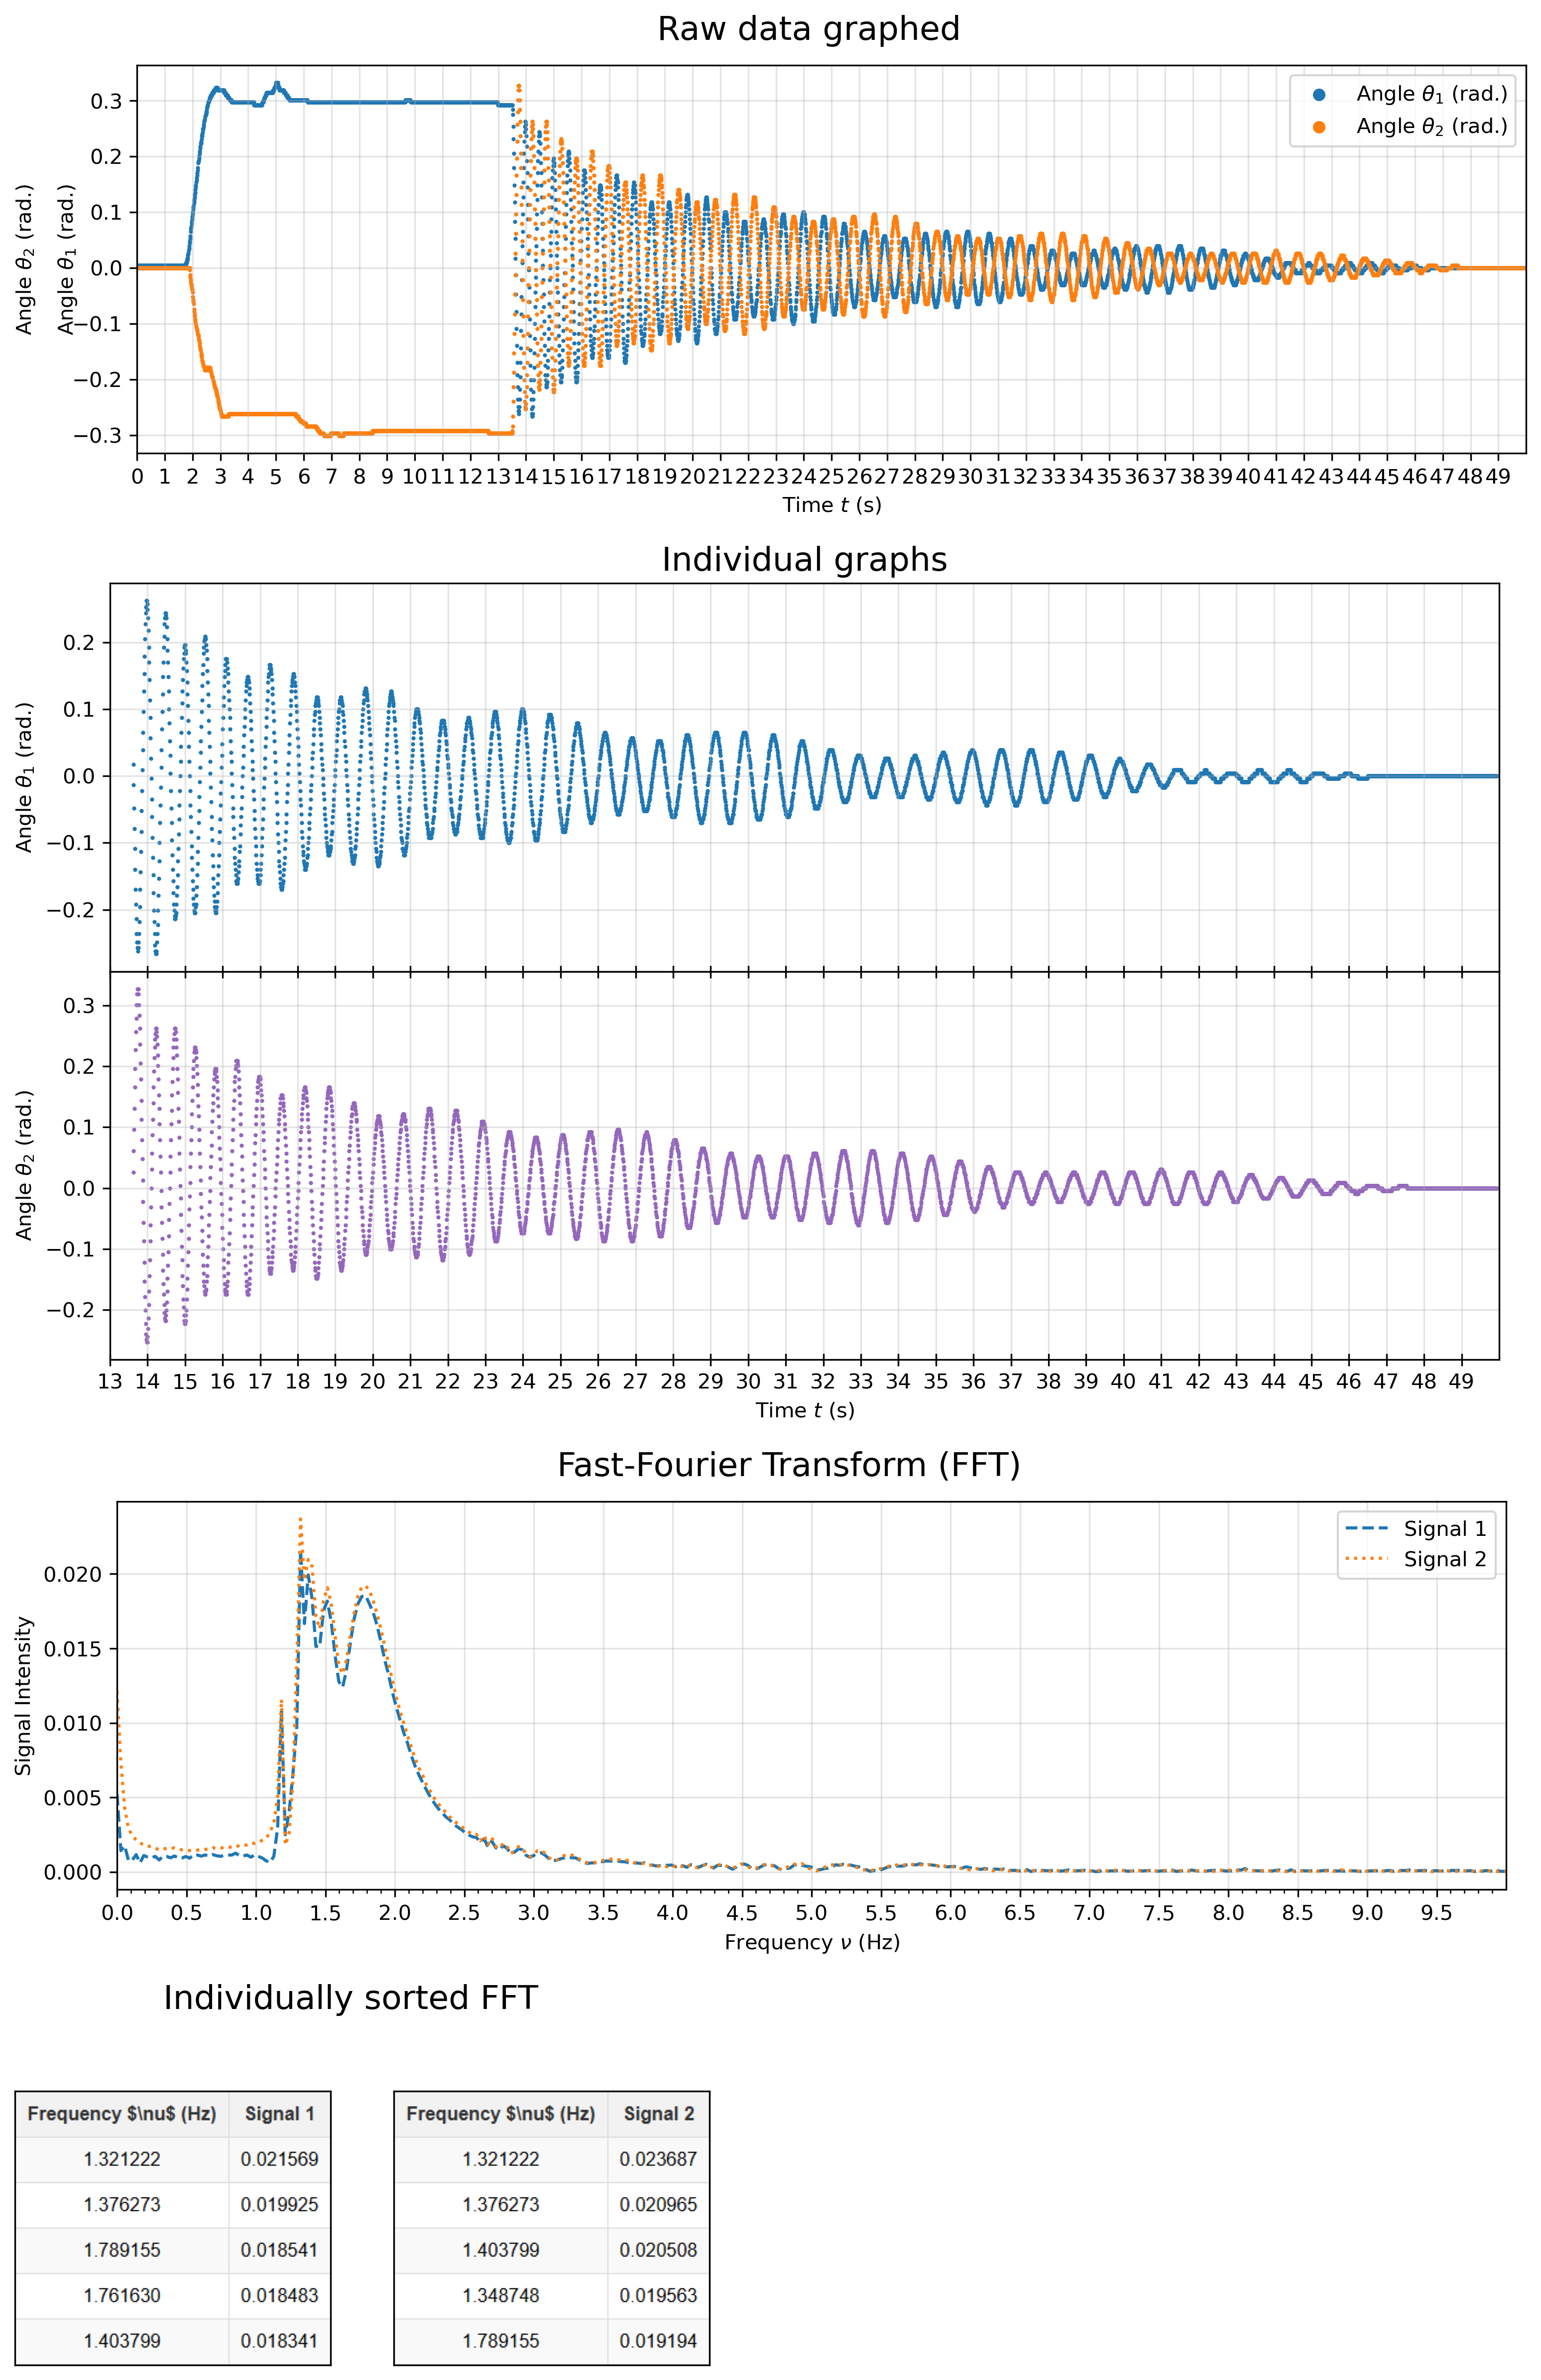
\includegraphics[width=0.98\linewidth]{figs/anti pendulum (right-back_3).png}
        \caption{Last trial done for the antisymmetric mode}
    \end{subfigure}
    \captionsetup{labelformat=empty} % last figure "hack" broke the numbering
    \caption{Figure 8: FFT analysis report for select antisymmetric mode coupled pendulums trial}
\end{figure}
\begin{multicols}{2}
\subsection{Conclusion}
Overall, the coupled pendulums experiment is a rich system with the potential to exhibit a myriad of waveforms for equally as rich physical analysis.
In hindsight after analyzing all data gathered for this paper, the initial conditions set for each trial typically was too large of an angular displacement.
Small-angle approximation according to one source is accurate up to 0.26 $\radian$ (or 15$^\circ$)---
all trials have initial conditions that exceed this value [\hyperref[sec:7]{7}].
This unaccounted error is the most likely reason behind some of the uncertainties reported throughout section \textbf{6 Results in Discussion}.
For future studies, it may be interesting to compare some of the results, either theoretical or experimental, to simulated results,
with one avenue to explore being to numerically approximate the equations of motion from the \textit{formal} Lagrangian of the system using an ordinary-differential-equations solver such as Runge-Kutta, Taylor series approximation, \textit{etc.}

\end{multicols}
\newpage

\subsection*{References}
\begin{enumerate}[label={[\arabic*]}]
    \item \label{sec:1} Department of Physics, New York University, ``Coupled Pendulum'', (2017). \url{https://physics.nyu.edu/~physlab/GenPhysII_PhysIII/Intermediate_Physics_I_writeups/Coupled-Pendulum_08-10-017.pdf}
    \item \label{sec:2} Taylor, John R. ``Classical Mechanics'' (University Science Books, 2003)
    \item \label{sec:3} For the Love of Physics. ``Coupled Pendulum - Normal Modes \& Frequencies $\vert$ Lagrangian Approach''. \textit{YouTube}, (2021). \url{https://www.youtube.com/watch?v=M-hLBxx7MeE}
    \item \label{sec:4} Herman, Russel. ``3.5: Nonlinear Pendulum''. \textit{LibreTexts\textsuperscript{TM} MATHEMATICS}, (University of North Carolina Wilmington, n.d.). \url{https://math.libretexts.org/Bookshelves/Differential_Equations/A_Second_Course_in_Ordinary_Differential_Equations%3A_Dynamical_Systems_and_Boundary_Value_Problems_(Herman)/03%3A_Nonlinear_Systems/3.05%3A_Nonlinear_Pendulum}
    \item \label{sec:5} Weisstein, Eric W. ``Fourier Transform''. \textit{MathWorld--- A Wolfram Web Resource}. \url{https://mathworld.wolfram.com/FourierTransform.html}
    \item \label{sec:6} The SciPy community. ``Fourier Transforms (\texttt{scipy.fft})''. \textit{SciPy}. \url{https://docs.scipy.org/doc/scipy/tutorial/fft.html}
    \item \label{sec:7} Farvard, Alireza \& Chesnutt, Betsy. ``Small Angle Approximation $\vert$ Overview, Formulas \& Applications''. \textit{Study.com} (2023). \url{https://study.com/academy/lesson/small-angle-approximation-formula-examples.html}
\end{enumerate}

%%%%%%%%%%%%%%%%%%%
% FIGURES (debug) %
%%%%%%%%%%%%%%%%%%%
% \newpage
% \begin{multicols}{2}

% \begin{figure}[H]
%     \centering
%     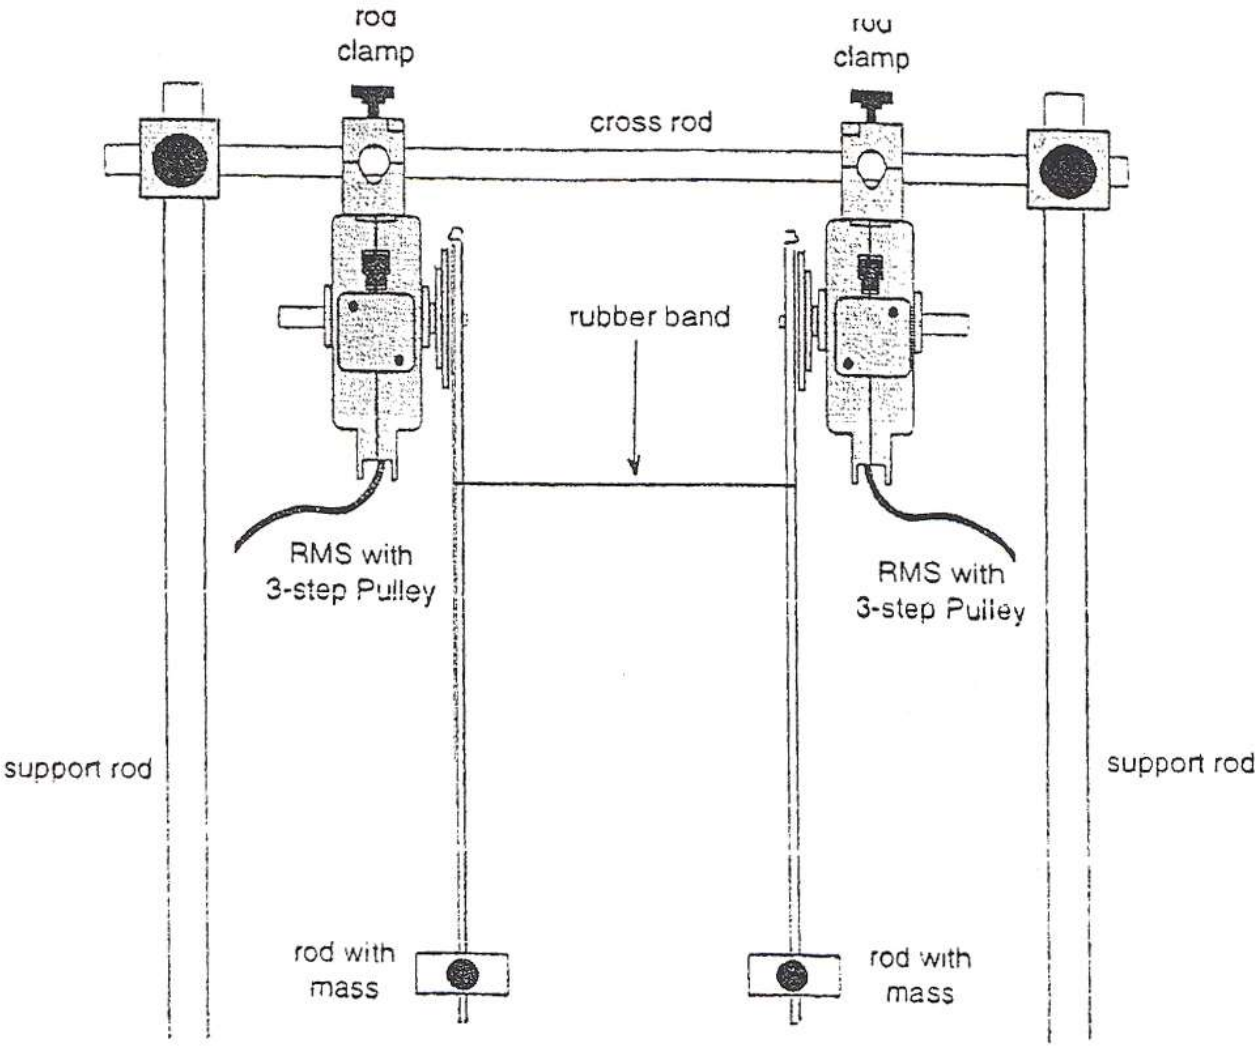
\includegraphics[width=0.98\linewidth]{figs/fig1_cropped.png}
%     \caption{Schematic illustration of the coupled pendulums lab setup [\hyperref[sec:1]{1}]}
%     \label{fig:1}
% \end{figure}

% \begin{figure}[H]
%     \centering
%     \begin{subfigure}{0.32\linewidth}
%         \centering
%         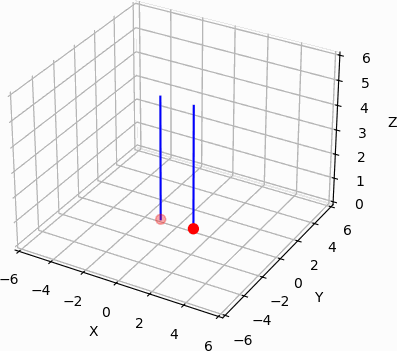
\includegraphics[width=0.98\linewidth]{figs/fig2/a_cropped.png}
%         \caption{}
%     \end{subfigure}
%     \begin{subfigure}{0.32\linewidth}
%         \centering
%         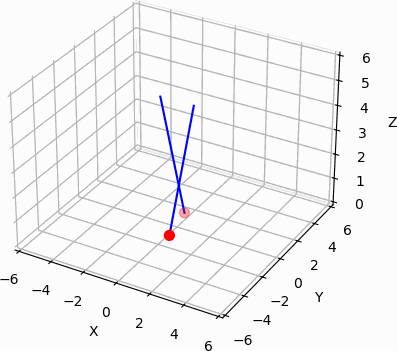
\includegraphics[width=0.98\linewidth]{figs/fig2/b_cropped.png}
%         \caption{}
%     \end{subfigure}
%     \begin{subfigure}{0.32\linewidth}
%         \centering
%         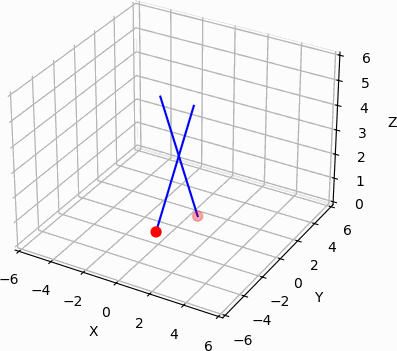
\includegraphics[width=0.98\linewidth]{figs/fig2/c_cropped.png}
%         \caption{}
%     \end{subfigure}
%     \begin{subfigure}{0.32\linewidth}
%         \centering
%         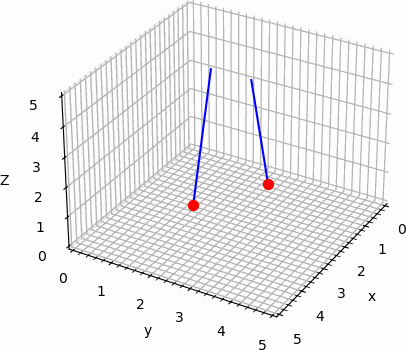
\includegraphics[width=0.98\linewidth]{figs/fig2/d_cropped.png}
%         \caption{}
%     \end{subfigure}
%     \begin{subfigure}{0.32\linewidth}
%         \centering
%         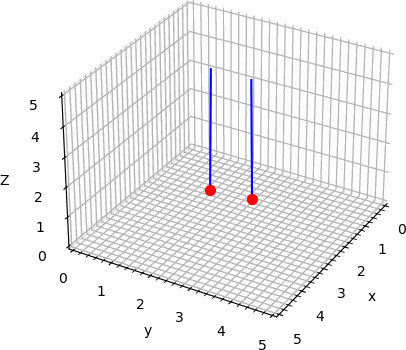
\includegraphics[width=0.98\linewidth]{figs/fig2/e_cropped.png}
%         \caption{}
%     \end{subfigure}
%     \begin{subfigure}{0.32\linewidth}
%         \centering
%         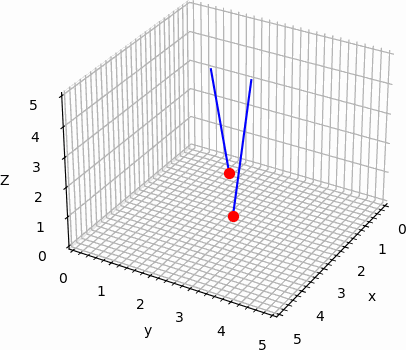
\includegraphics[width=0.98\linewidth]{figs/fig2/f_cropped.png}
%         \caption{}
%     \end{subfigure}
%     \caption{
%         Frames of motion for various degrees of freedom.
%         (a), (b), \& (c) depicts the pendulums sweeping a circle as an
%         example of \textit{two} degrees of freedom motion. (d), (e), \& (f)
%         depicts the pendulums swinging simply in parallel to the $x$-axis,
%         implying \textit{one} degree of freedom motion.
%     }
% \end{figure}

% \begin{figure}[H]
%     \centering
%     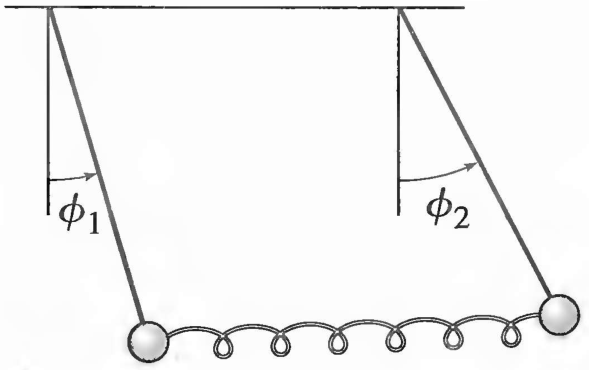
\includegraphics[width=0.98\linewidth]{figs/fig3_cropped.png}
%     \caption{
%         Alternative coupled pendulums problem as depicted in two-dimensions.
%         Adapted from \textit{Classical Mechanics}, by \textit{John R. Taylor} (2003),
%         \textit{Figure 11.17} [\hyperref[sec:2]{2}]
%     }
% \end{figure}

% \begin{figure}[H]
%     \centering
%     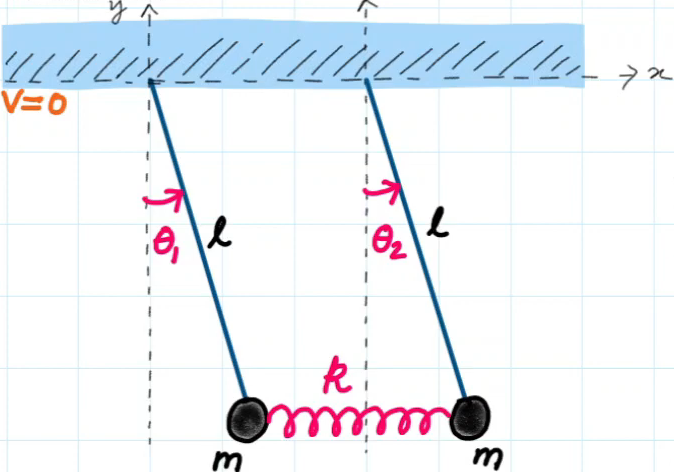
\includegraphics[width=0.98\linewidth]{figs/fig4_cropped_edited.png}
%     \caption{Drawn analysis of the simplified coupled pendulum problem [\hyperref[sec:3]{3}]}
% \end{figure}

% \begin{figure}[H]
%     \begin{tcolorbox}[ % nearly copied straight from Jupyter's exported file
%         breakable, size=fbox, boxrule=1pt, pad at break*=1mm,colback=cellbackground, colframe=cellborder
%     ]
%         \begin{lstlisting}[language=Python] 
% from scipy.fft import fft, fftfreq
% import numpy as np
% # Number of sample points
% N = 600
% # sample spacing
% T = 1.0 / 800.0
% x = np.linspace(0.0, N*T, N, endpoint=False)
% y = np.sin(50.0 * 2.0*np.pi*x) + 0.5*np.sin(80.0 * 
% (*@$\hookrightarrow$@*) 2.0*np.pi*x)
% yf = fft(y)
% xf = fftfreq(N, T)[:N//2]
% import matplotlib.pyplot as plt
% plt.plot(xf, 2.0/N * np.abs(yf[0:N//2]))
% plt.grid()
% plt.show()
%         \end{lstlisting} % interesting so margins do matter in this environment
%     \end{tcolorbox}
%     \caption{Example code of FFT from the \texttt{scipy} [\hyperref[sec:6]{6}]}
% \end{figure}

% \begin{figure*} % could also use the onecolumn environment
%     \centering
%     \begin{subfigure}{0.49\linewidth}
%         \centering
%         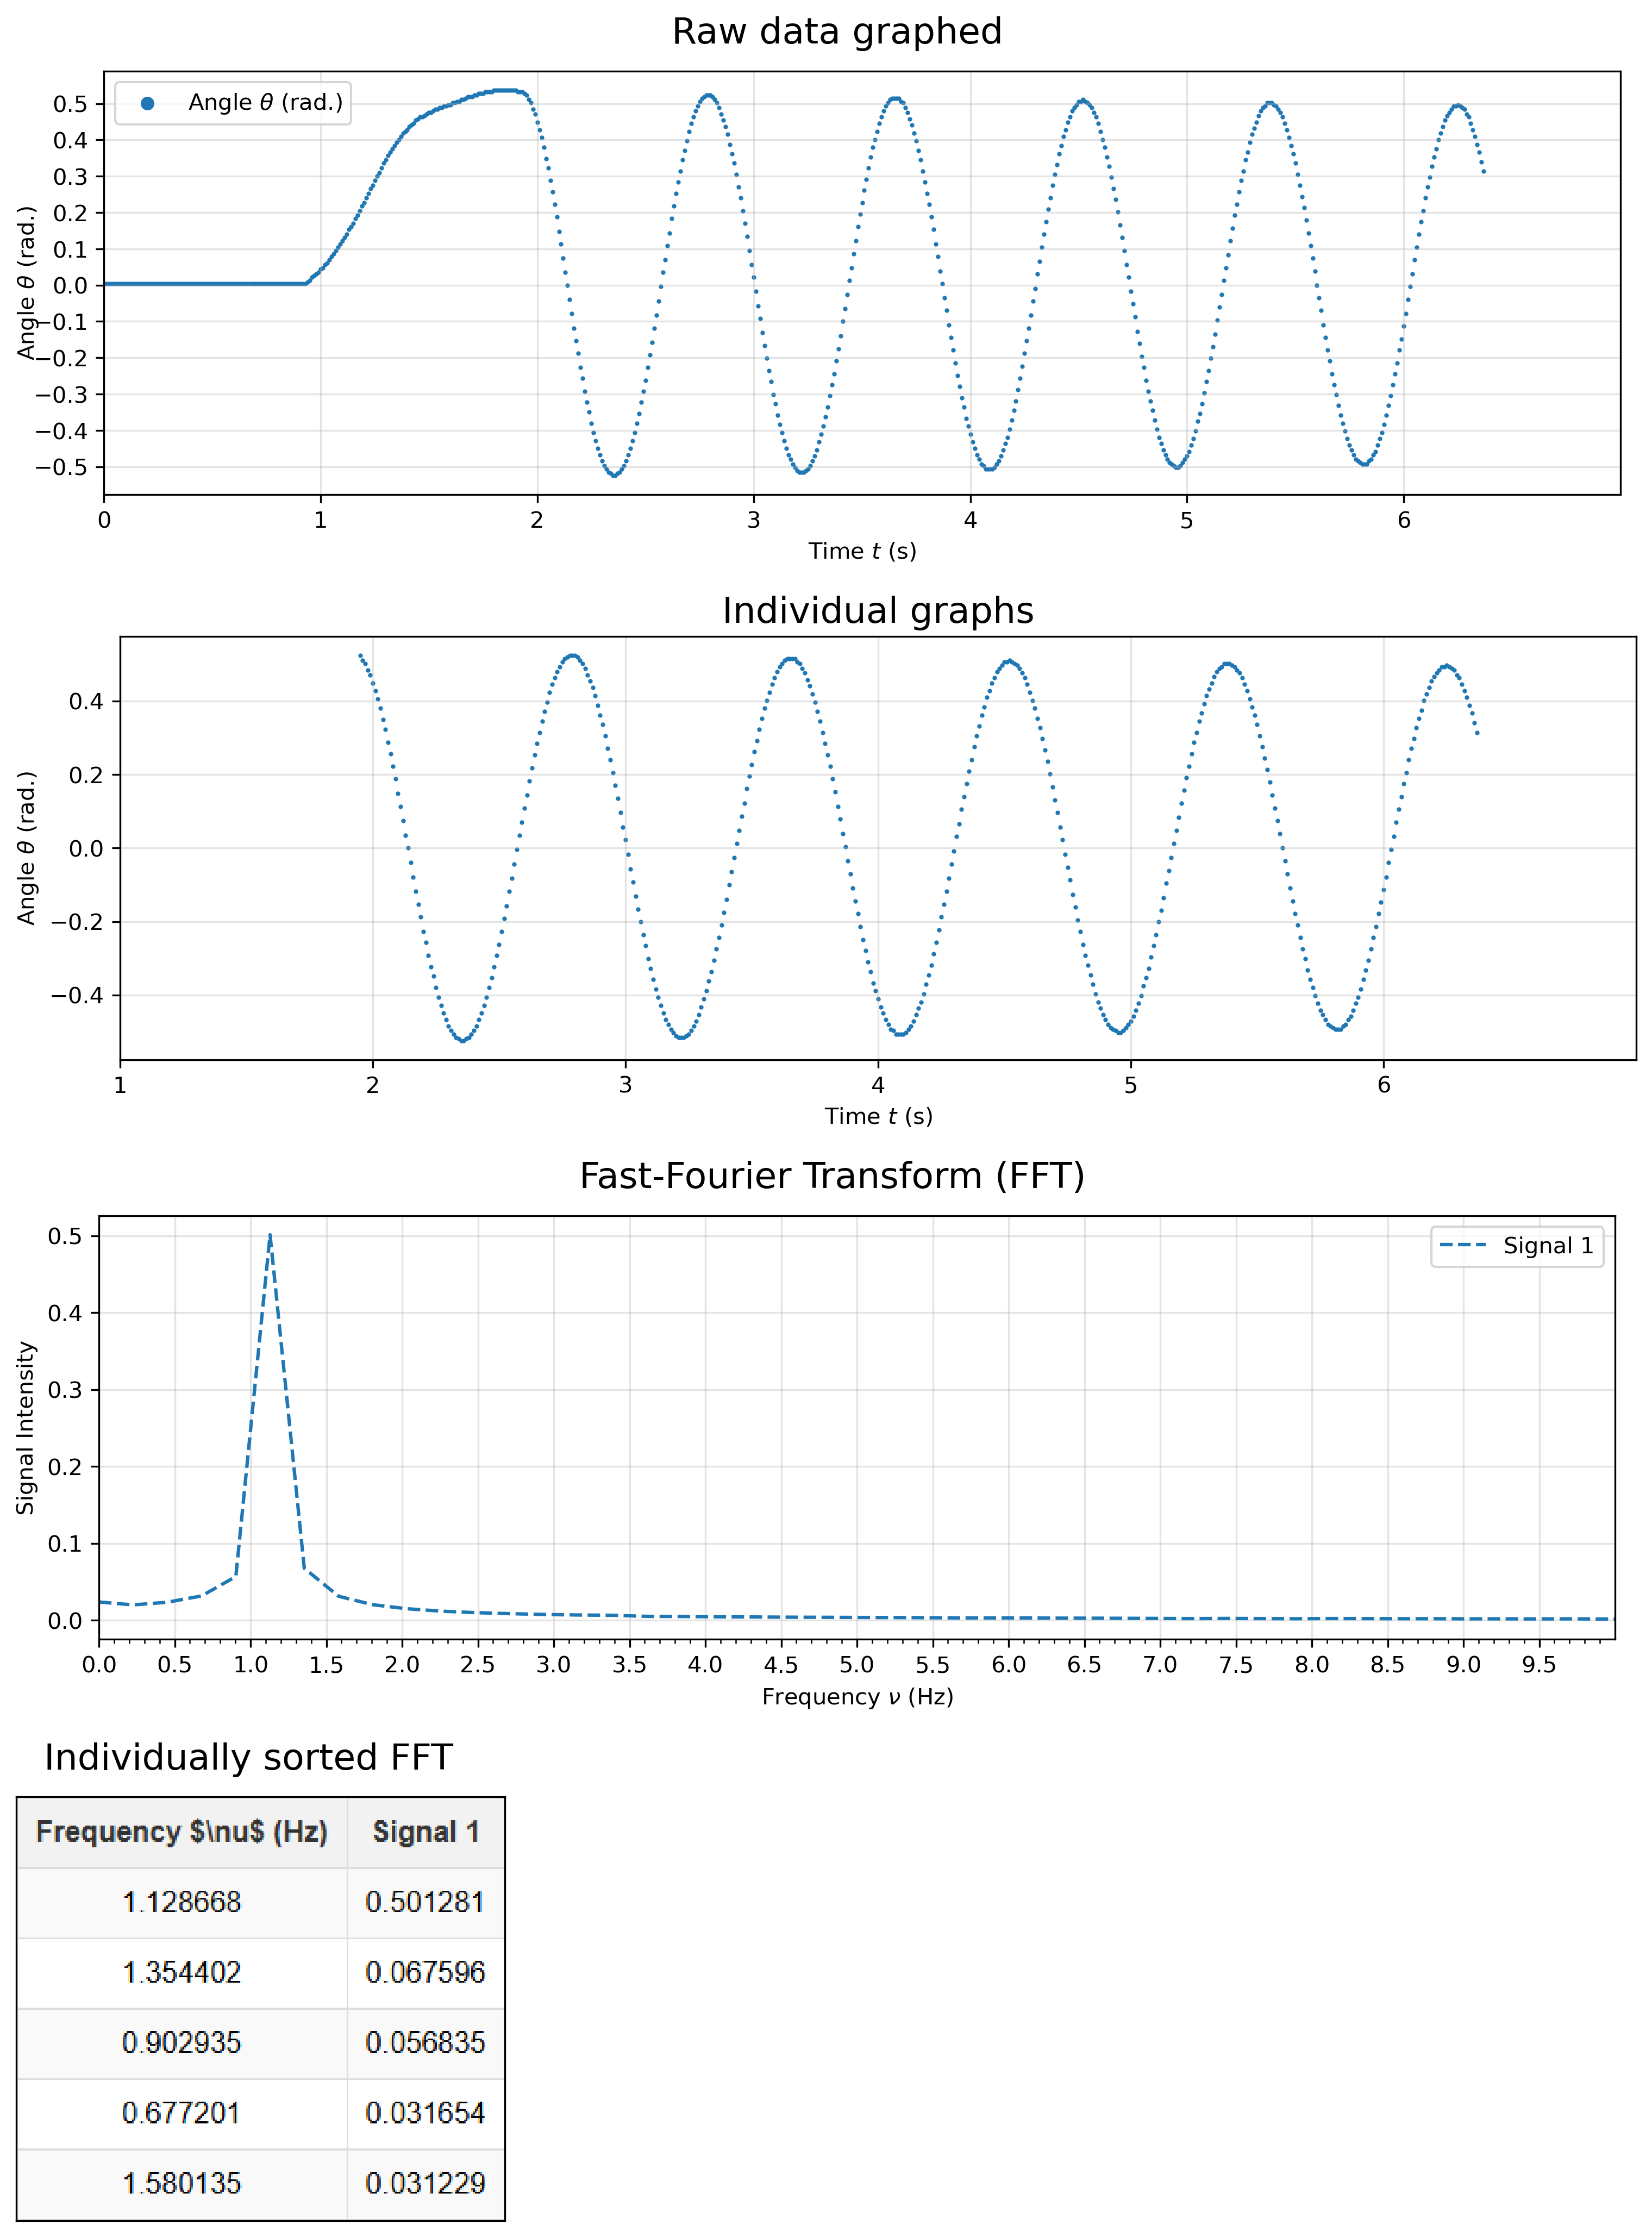
\includegraphics[width=0.98\linewidth]{figs/left pendulum trial 1.png}
%         \caption{Trial 1 of gathering left-pendulum oscillation data}
%     \end{subfigure}
%     \begin{subfigure}{0.49\linewidth}
%         \centering
%         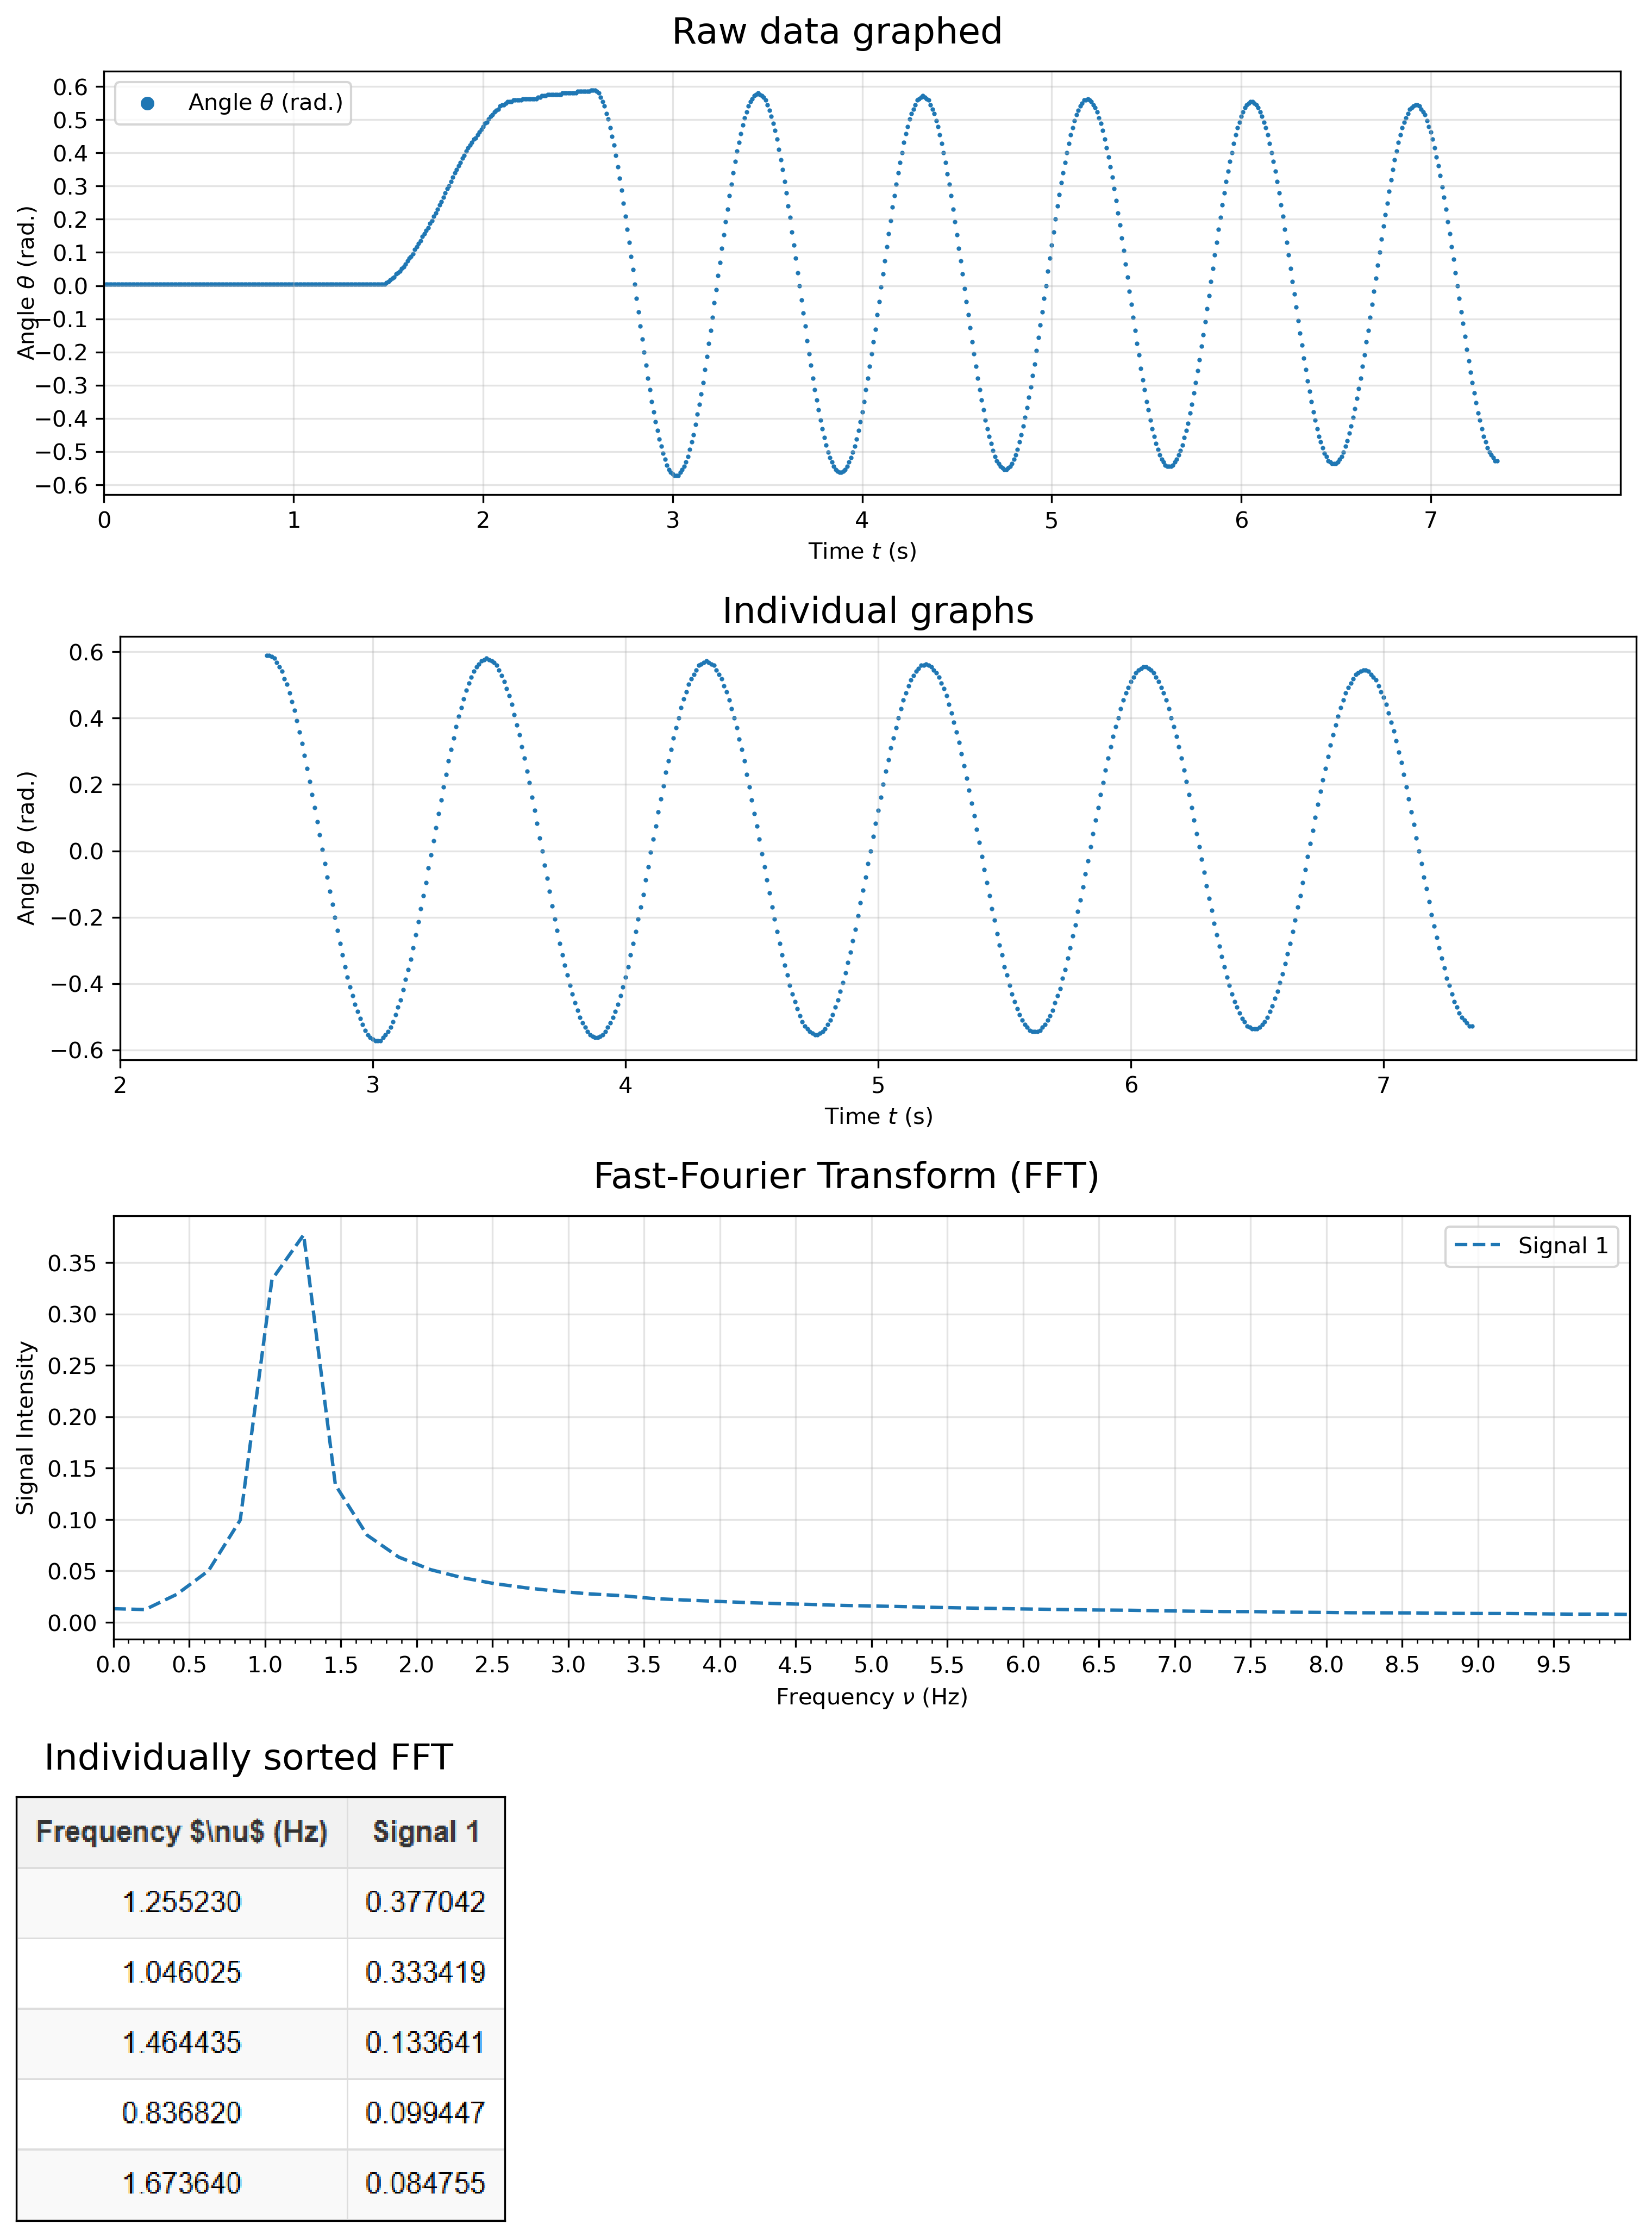
\includegraphics[width=0.98\linewidth]{figs/left pendulum trial 2.png}
%         \caption{Trial 2 of gathering left-pendulum oscillation data}
%     \end{subfigure}
%     \caption{Full analysis on the natural oscillations of the left pendulum of the apparatus}
% \end{figure*}

% \begin{figure*} % half of the figure
%     \centering
%     \begin{subfigure}{0.49\linewidth}
%         \centering
%         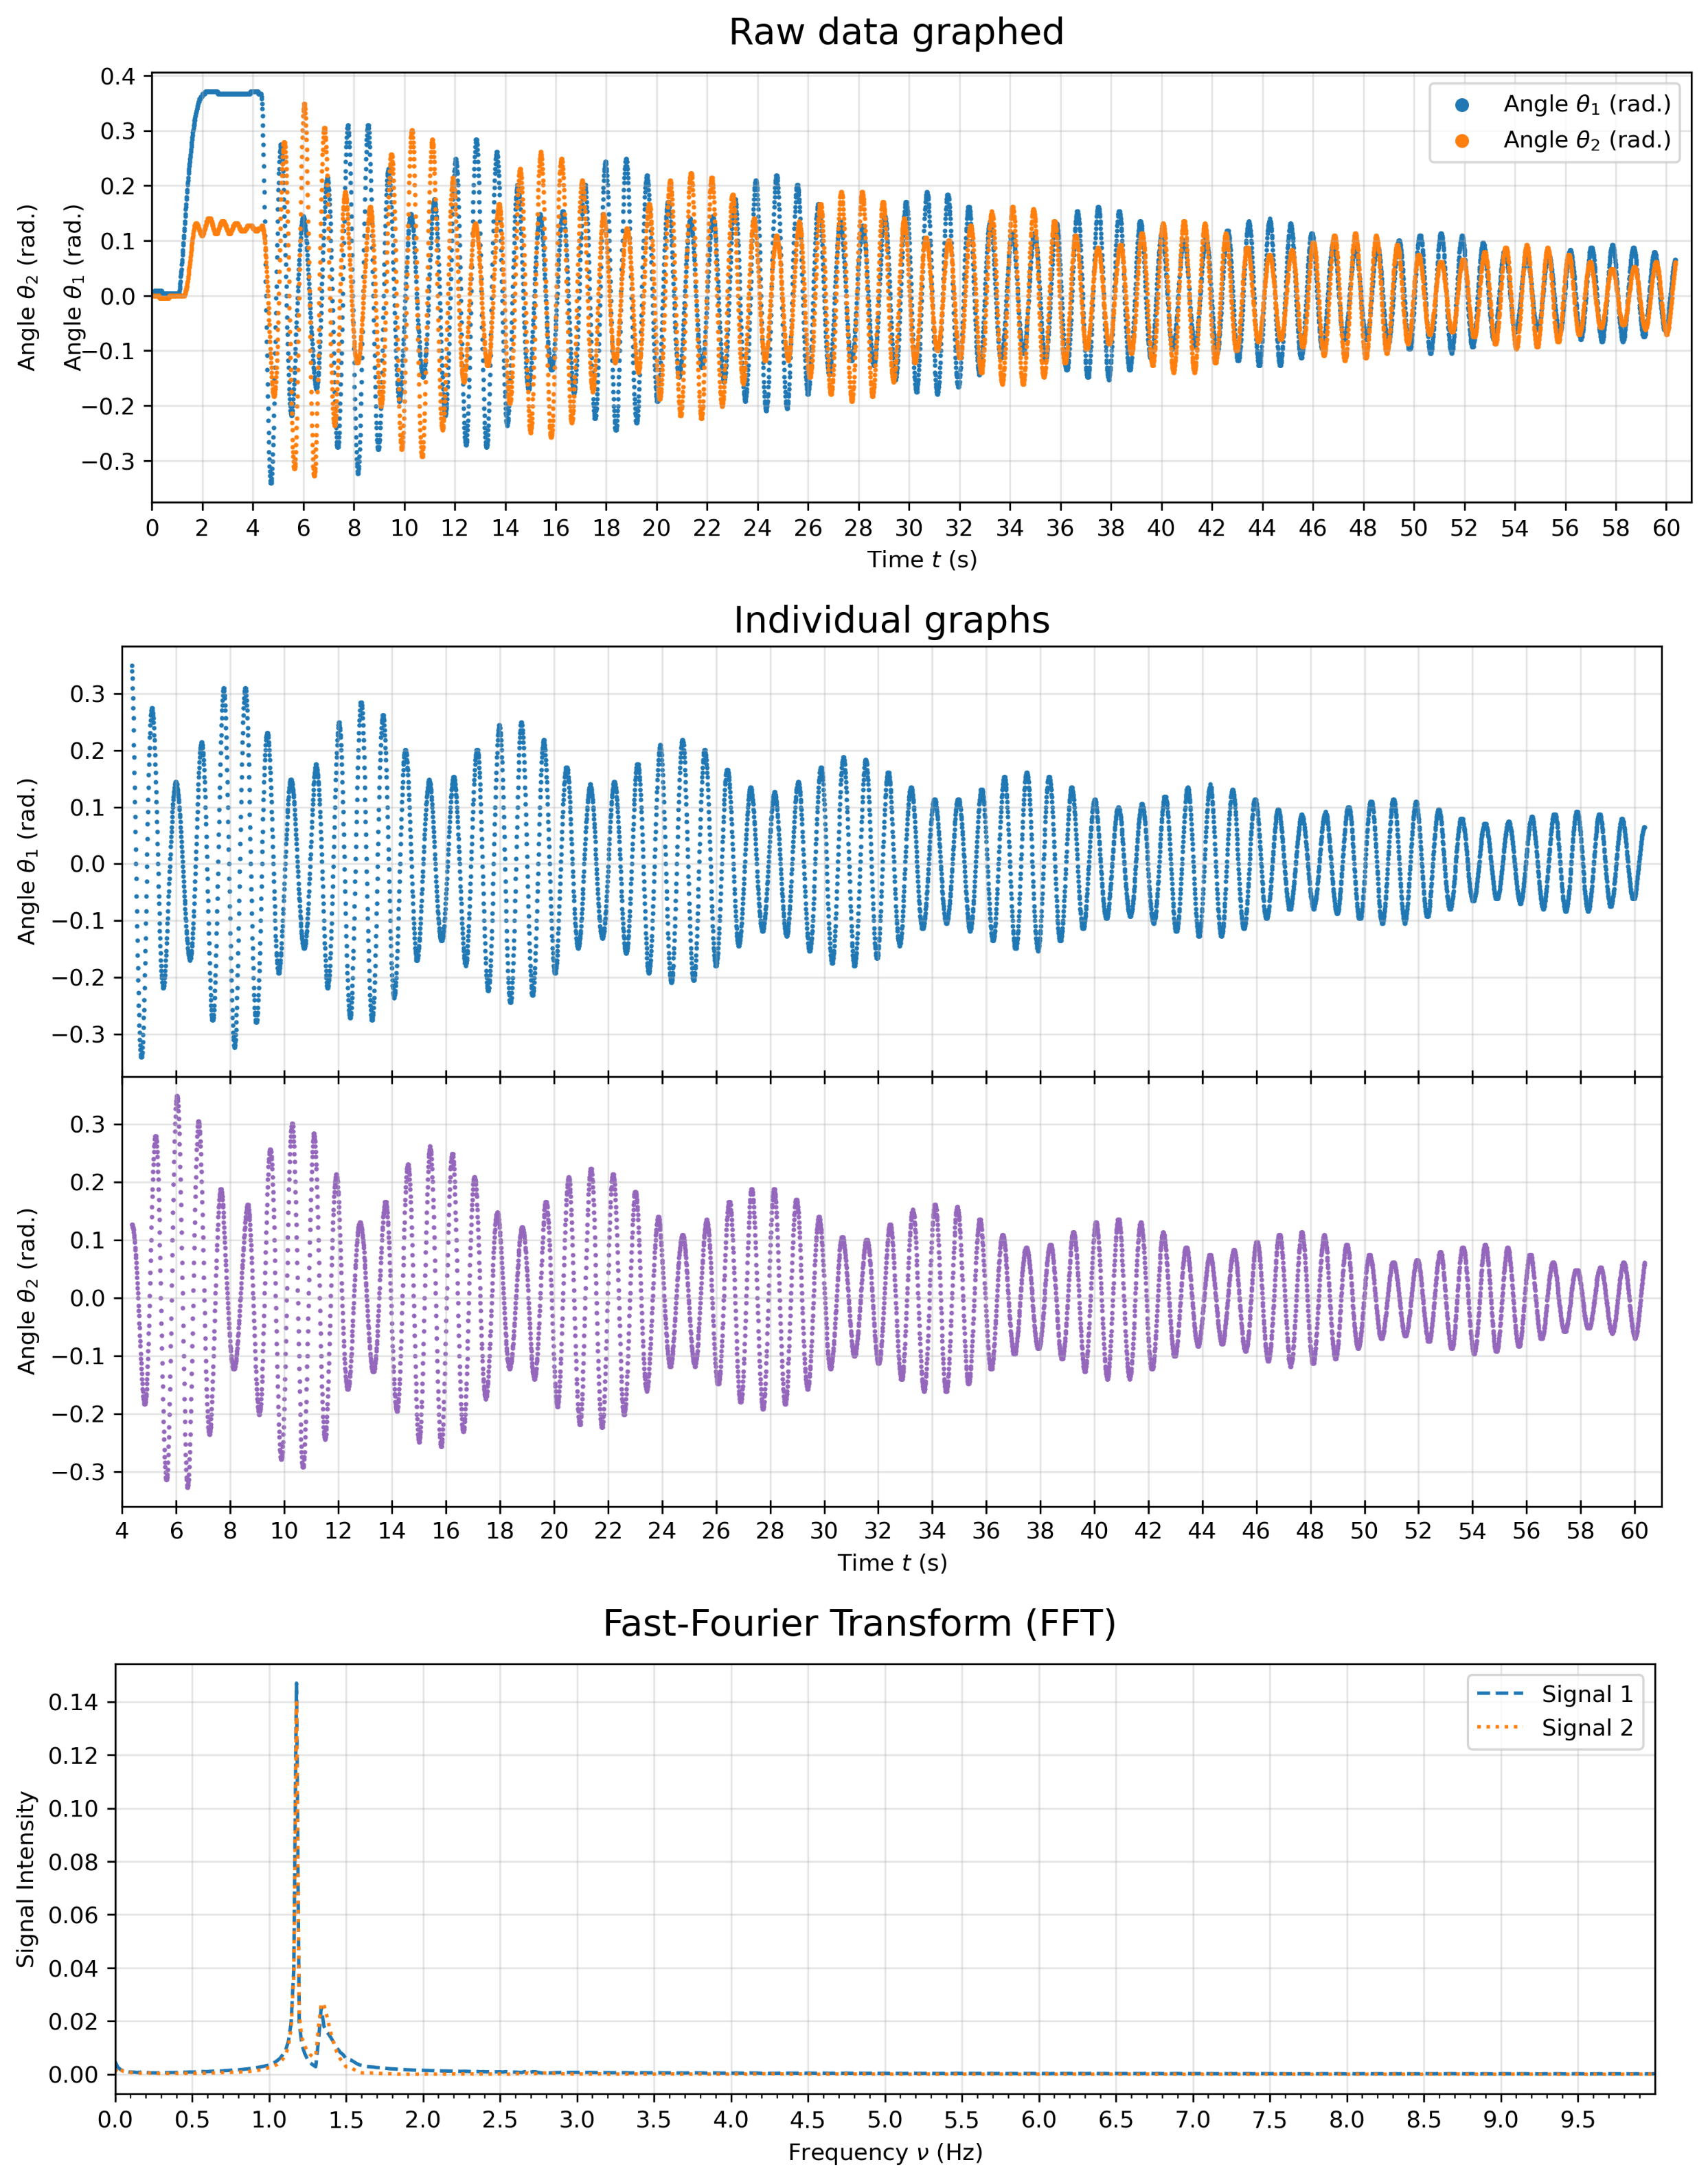
\includegraphics[width=0.98\linewidth]{figs/beat (left_9_3)_cropped.png}
%         \caption{Clearest FFT graph for 9 cm coupliing}
%     \end{subfigure}
%     \begin{subfigure}{0.49\linewidth}
%         \centering
%         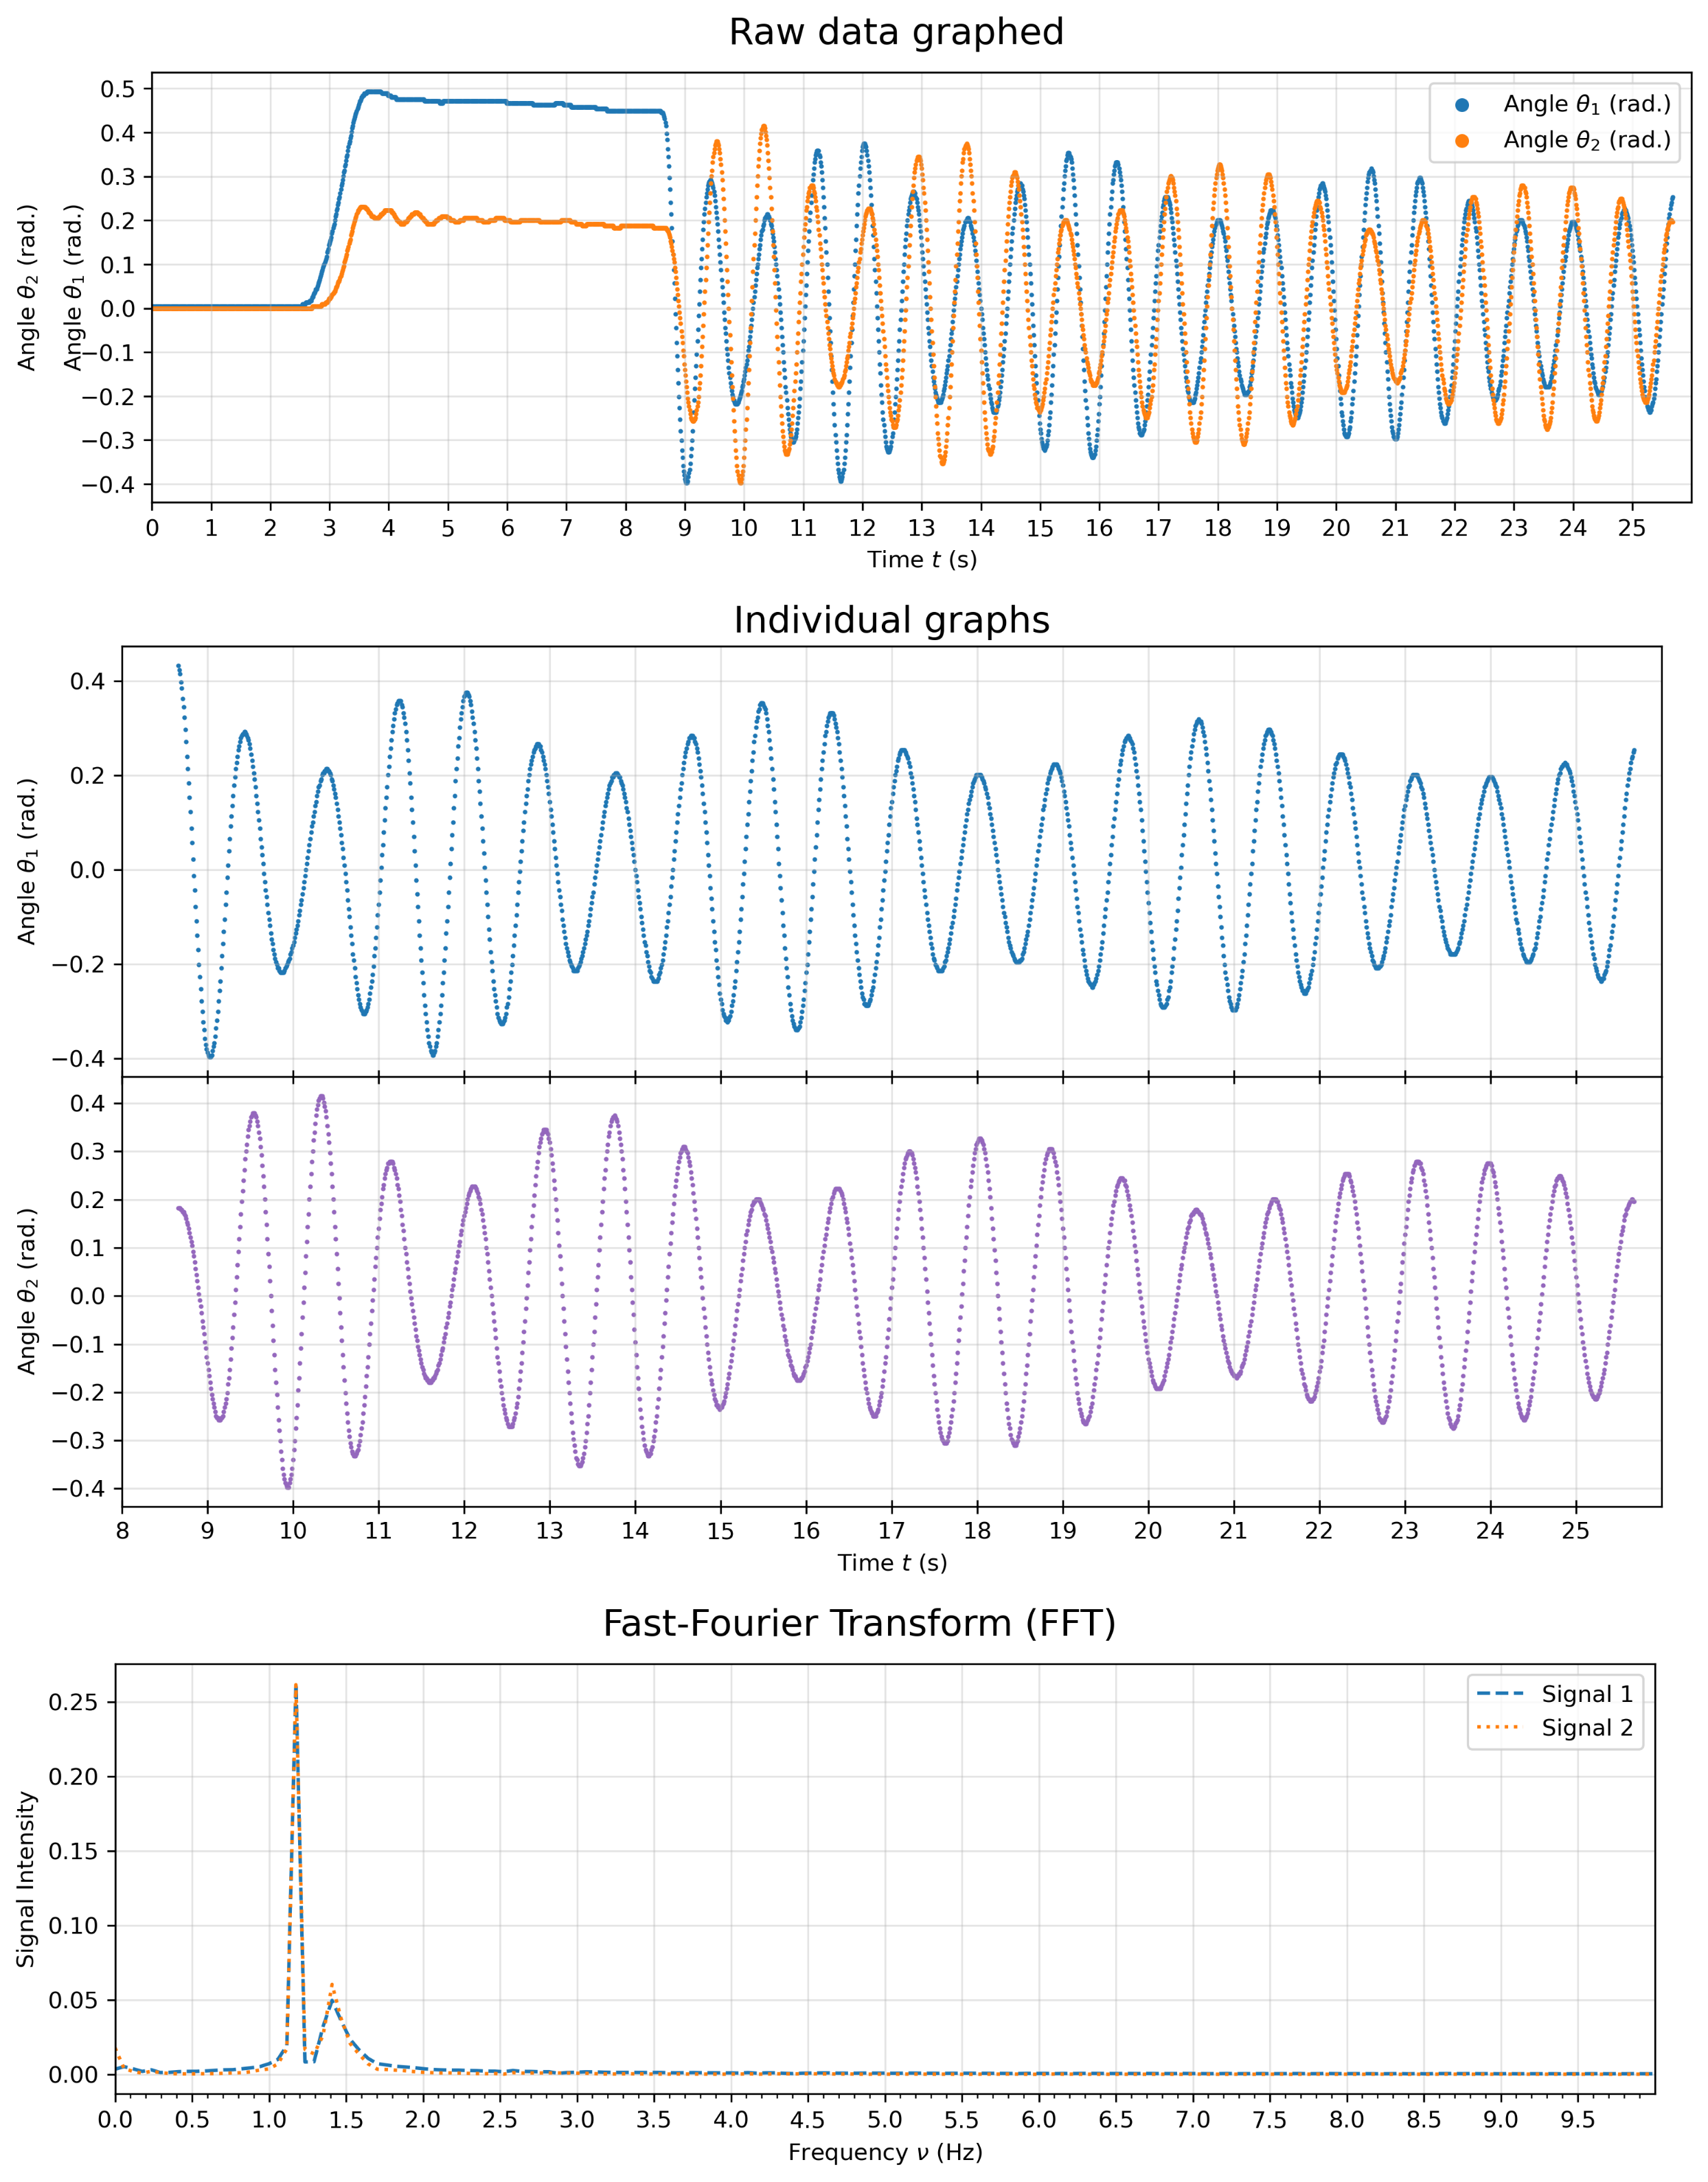
\includegraphics[width=0.98\linewidth]{figs/beat (left_9-5_1)_cropped.png}
%         \caption{Clearest FFT graph for 9$\sfrac{1}{2}$ cm coupliing}
%     \end{subfigure}
%     \caption{Best FFT analysis reports for 9 cm, 9$\sfrac{1}{2}$ cm, and 10 cm coupling settings}
% \end{figure*}

% \begin{figure}[H]
%     \centering
%     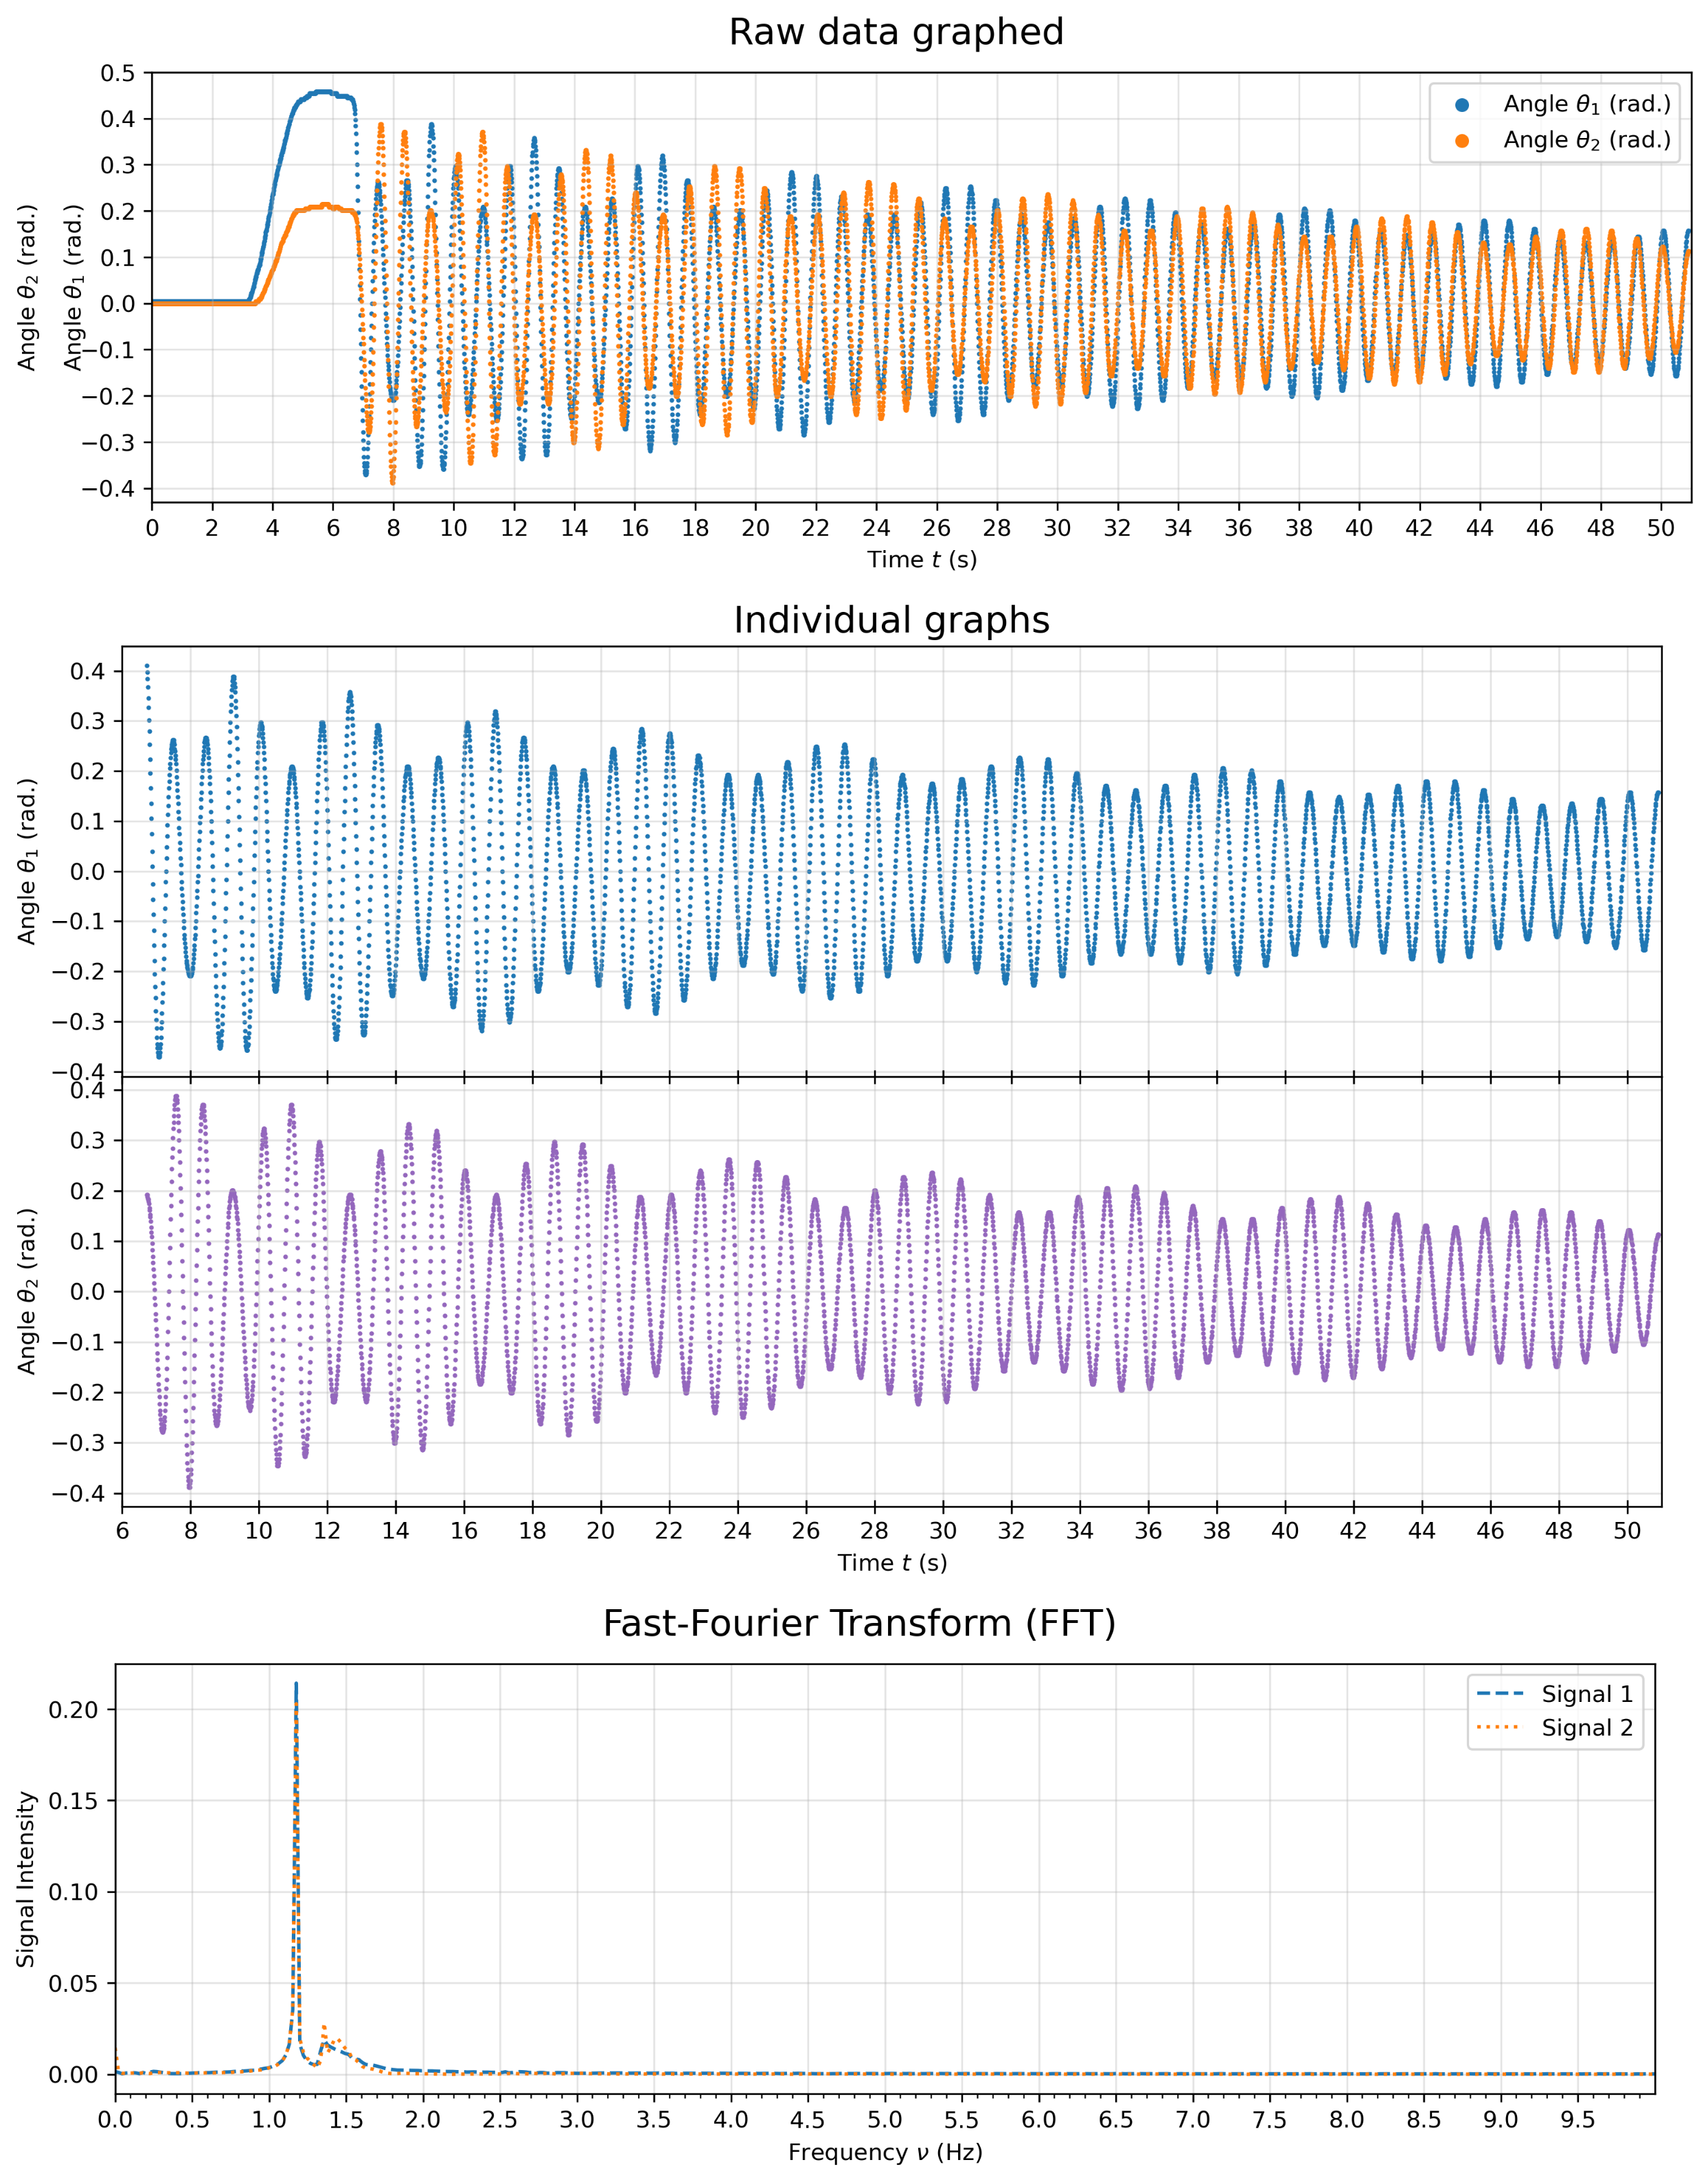
\includegraphics[width=0.98\linewidth]{figs/beat (left_10_2)_cropped.png}   
%     \captionsetup{labelformat=empty}
%     \caption{(c) Clearest FFT graph for 10 cm coupliing}
% \end{figure}

% \begin{figure*}
%     \centering
%     \begin{subfigure}{0.49\linewidth}
%         \centering
%         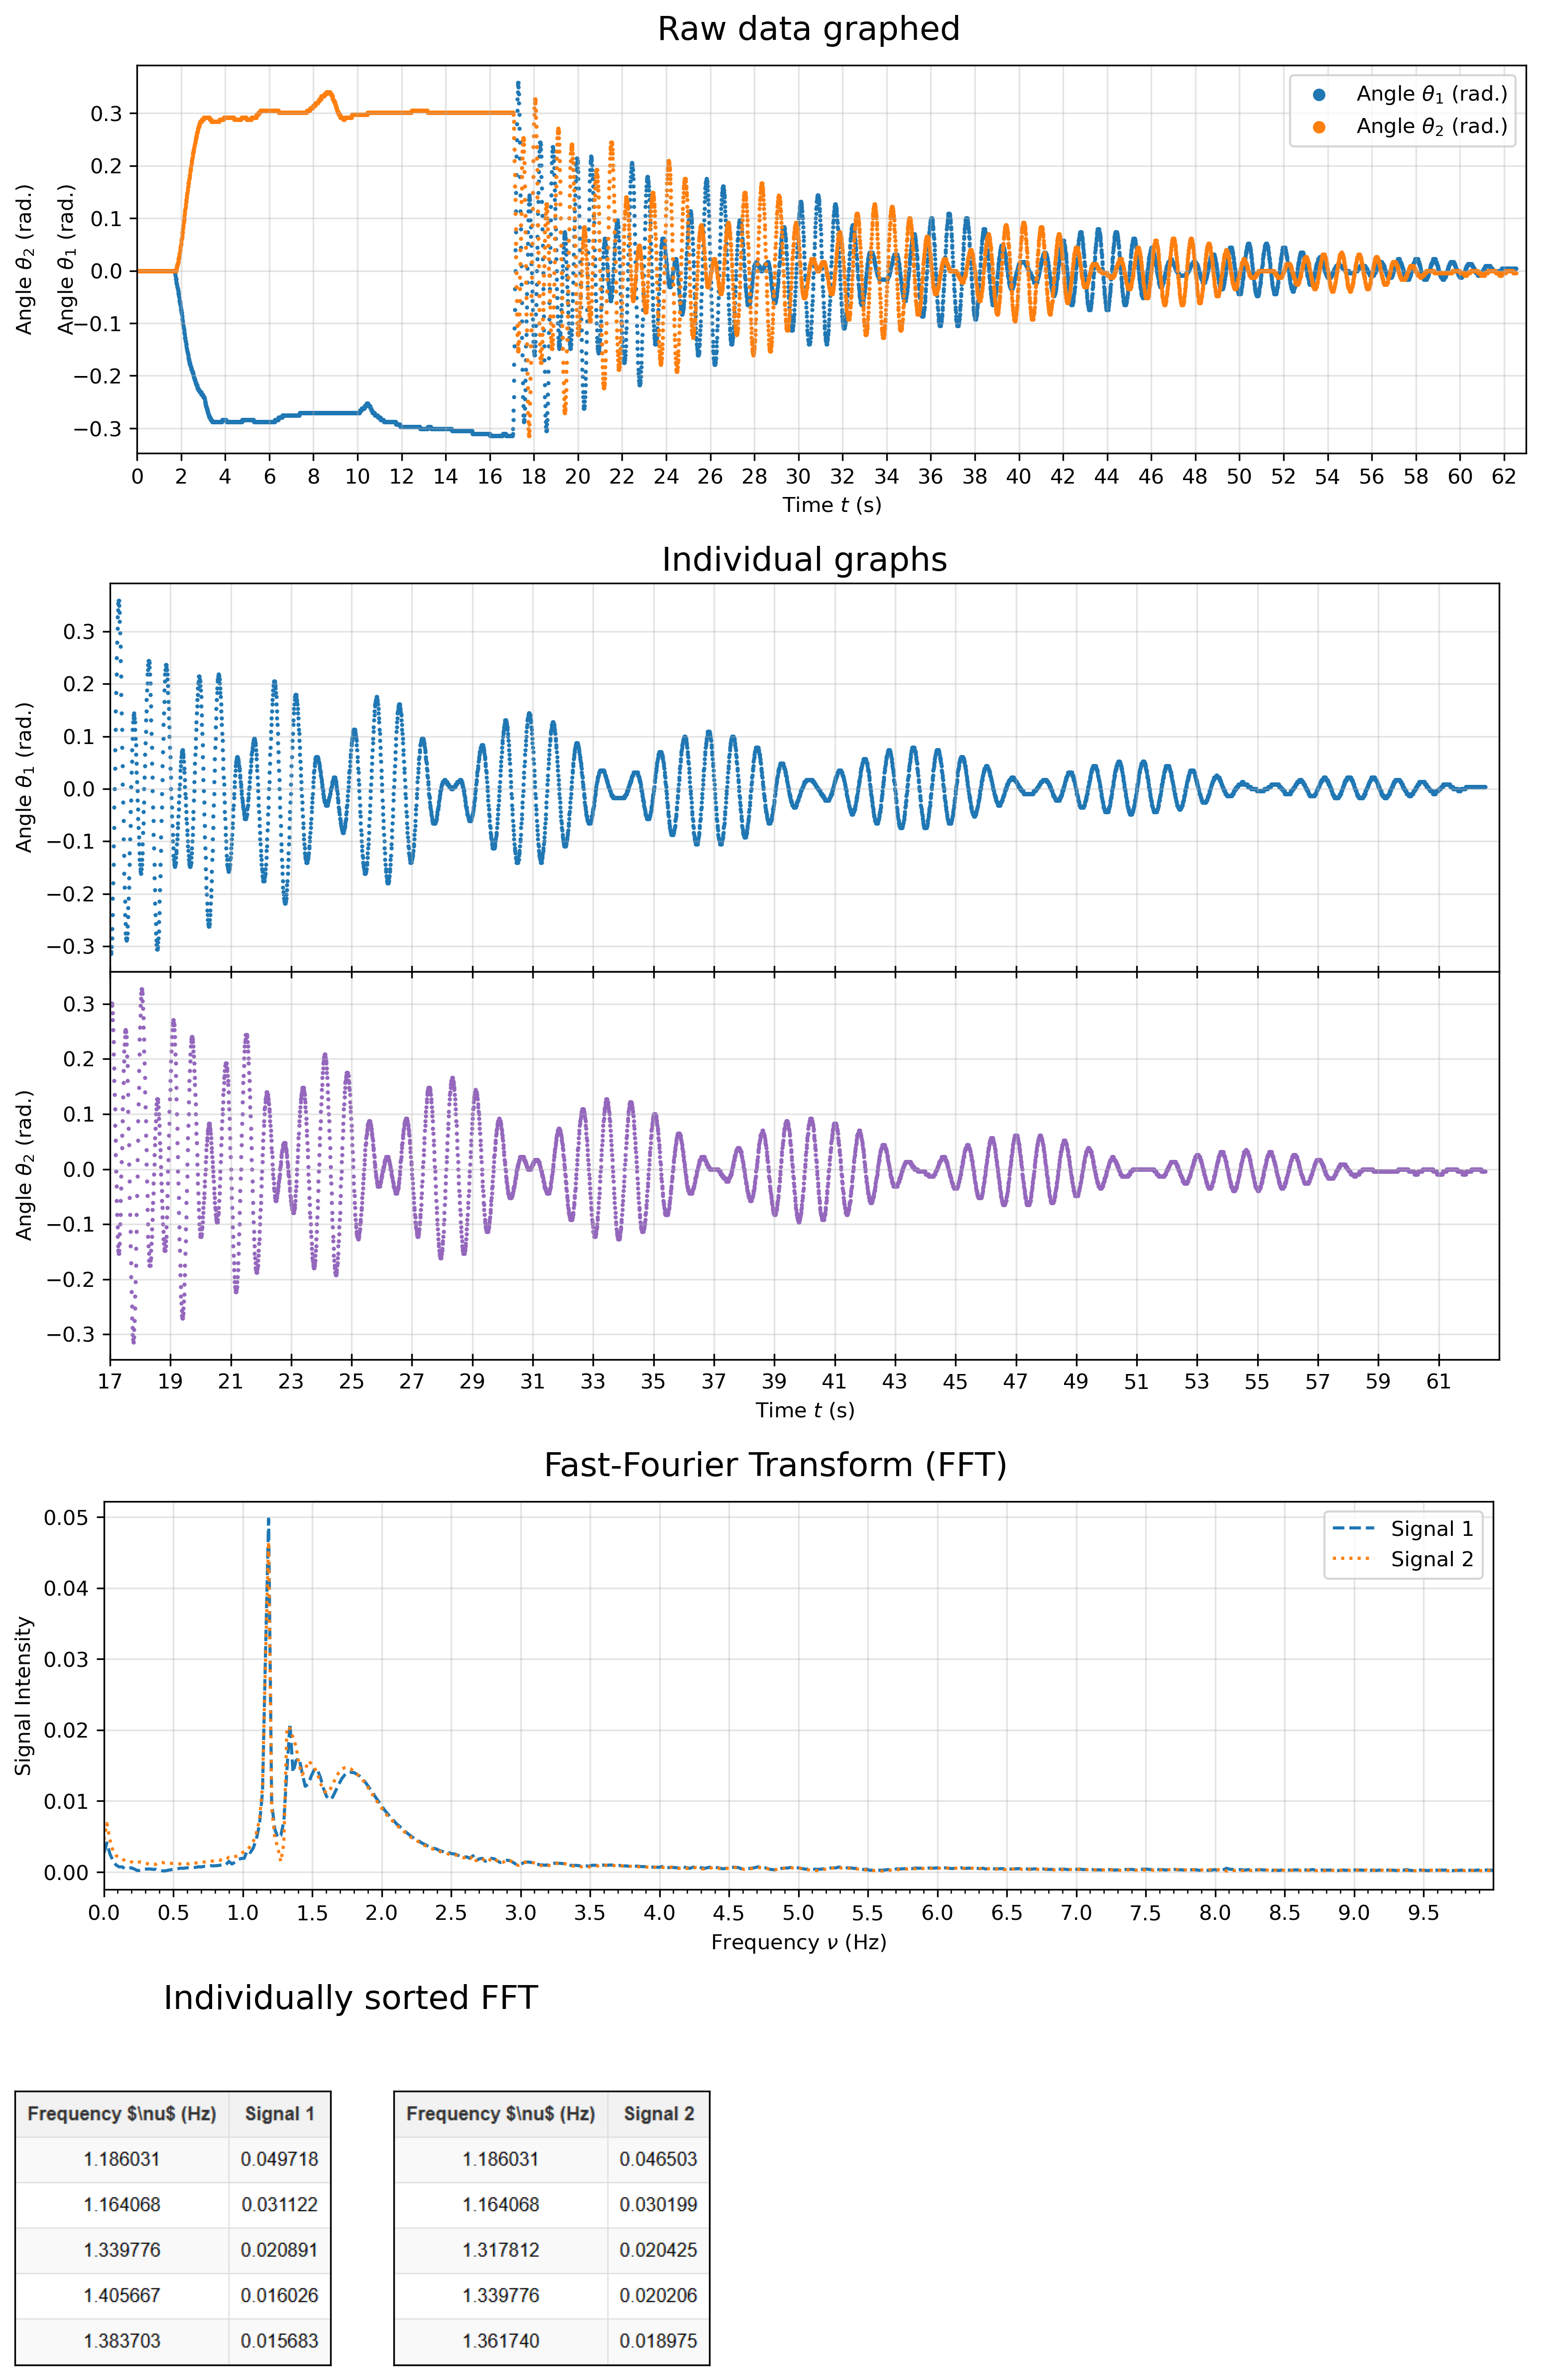
\includegraphics[width=0.98\linewidth]{figs/anti pendulum (left-back_1).png}
%         \caption{First trial done for the antisymmetric mode}
%     \end{subfigure}
%     \begin{subfigure}{0.49\linewidth}
%         \centering
%         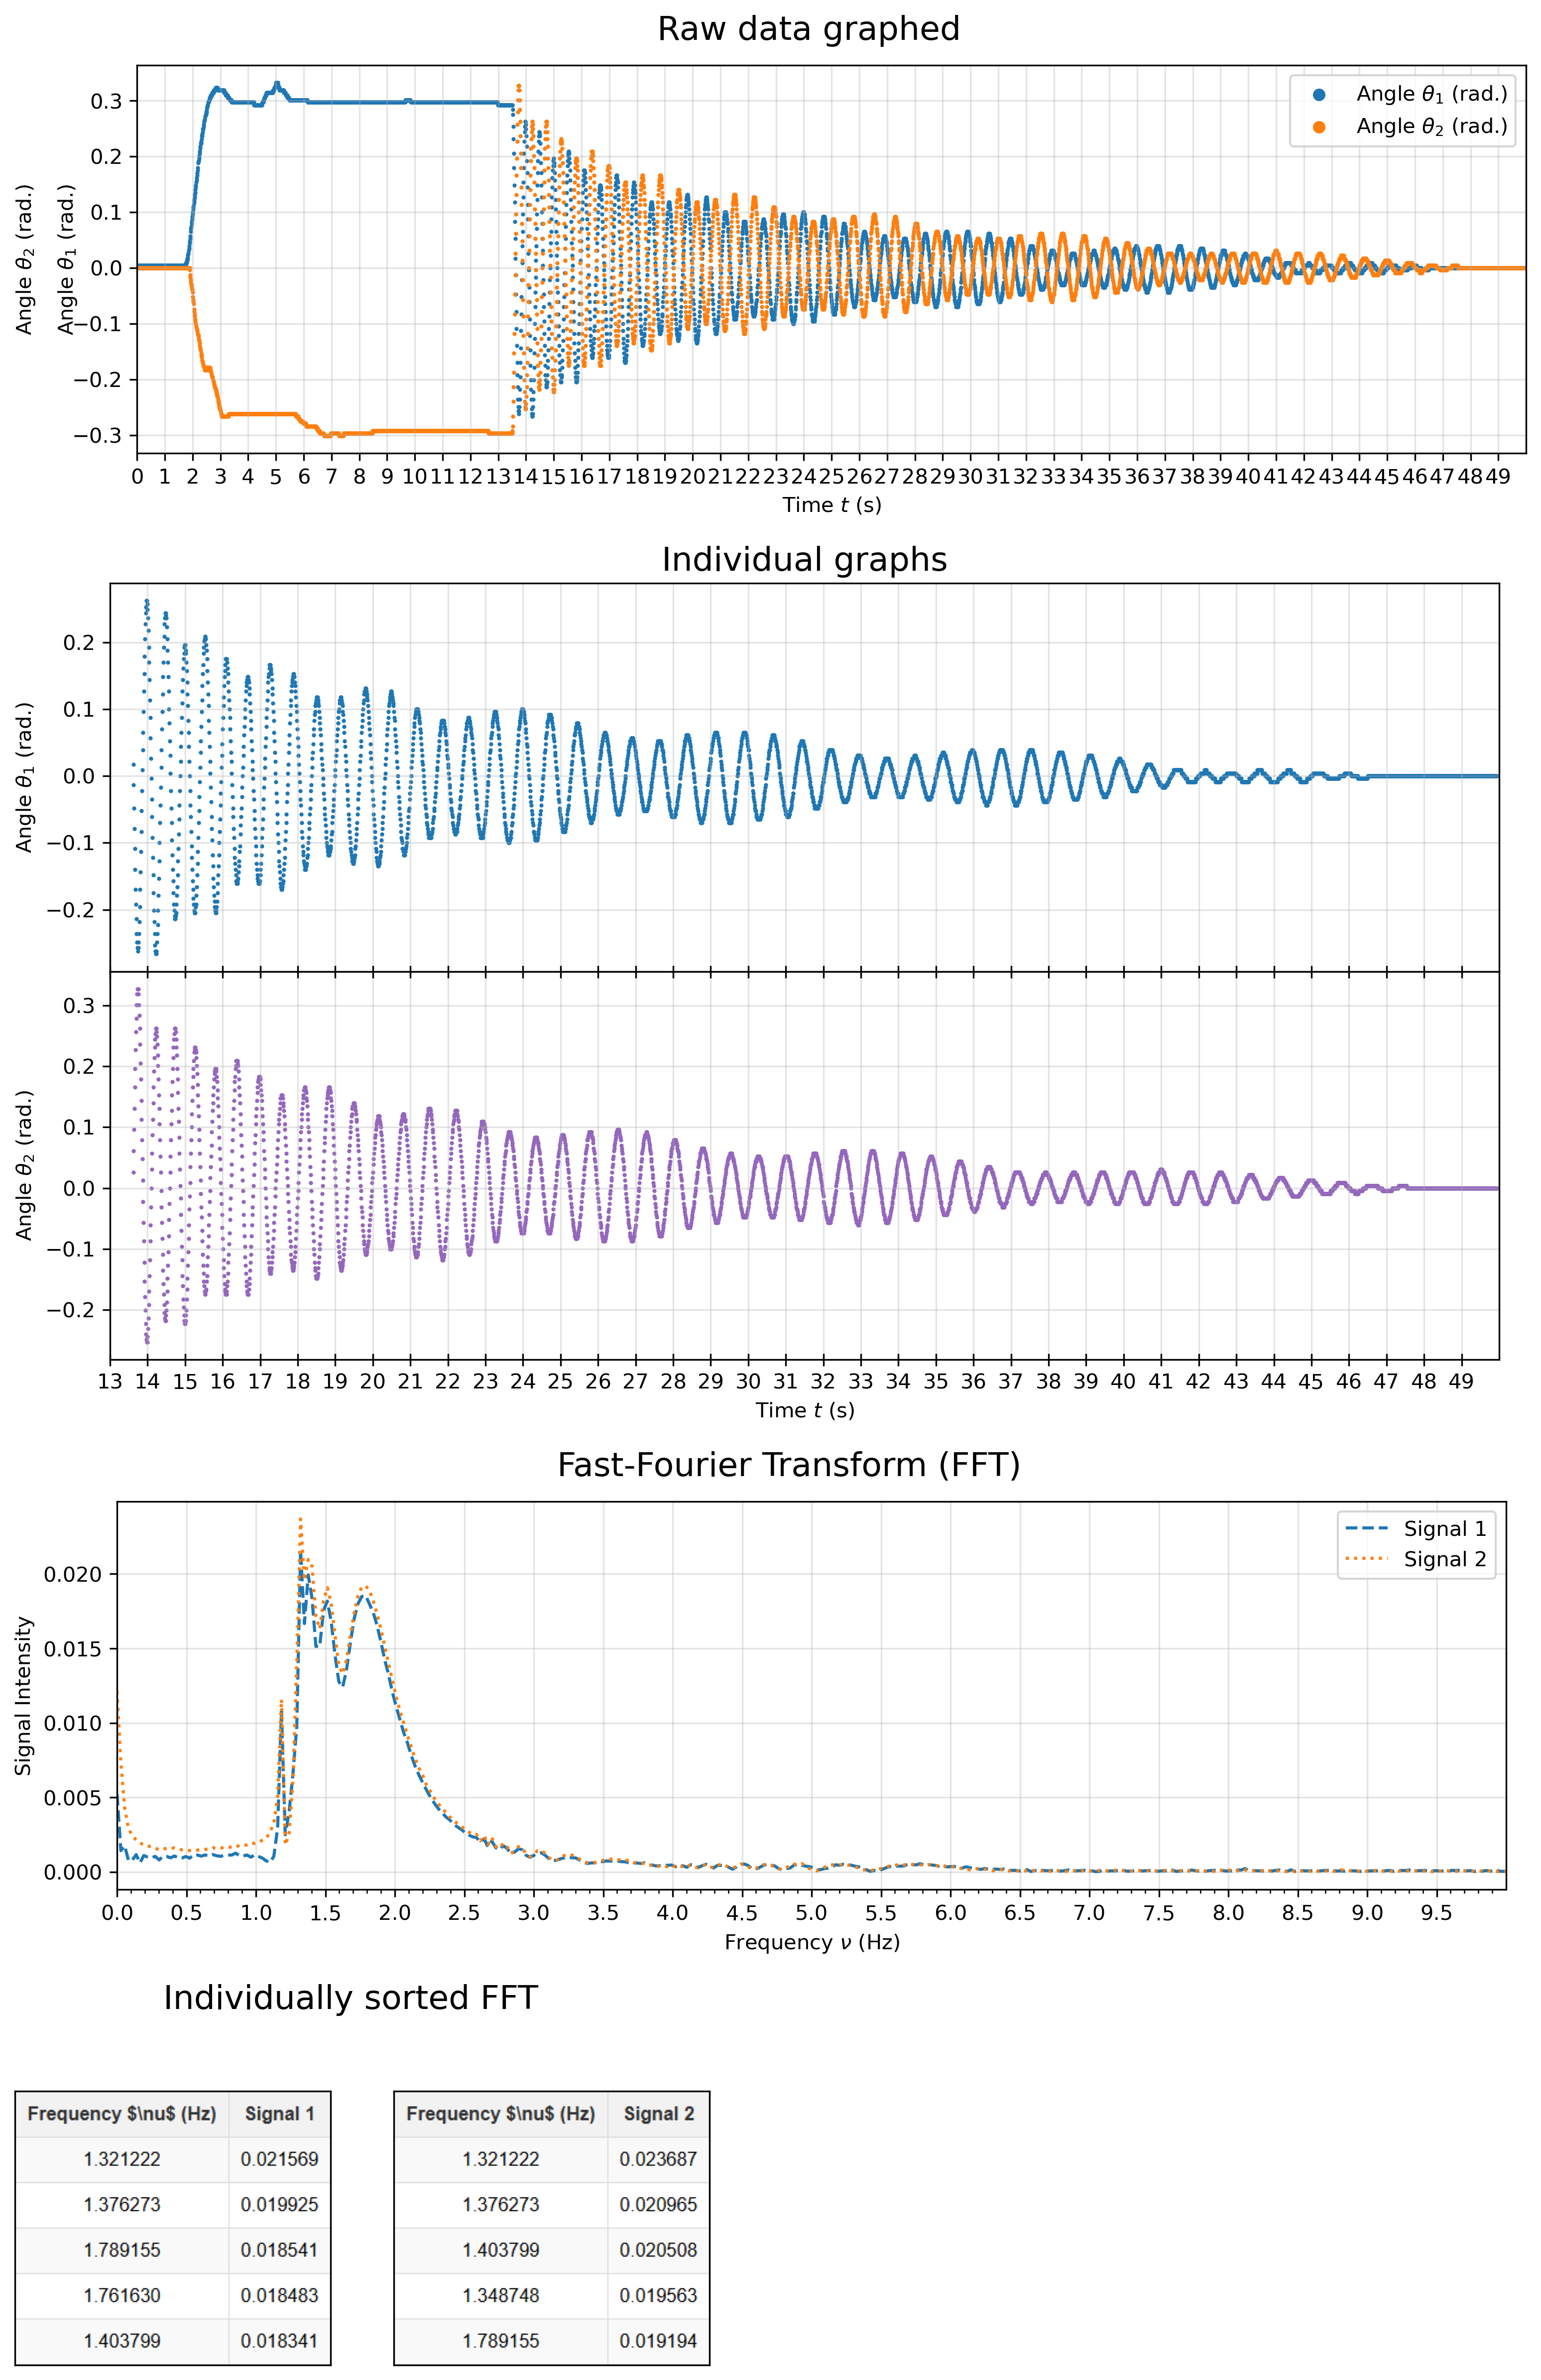
\includegraphics[width=0.98\linewidth]{figs/anti pendulum (right-back_3).png}
%         \caption{Last trial done for the antisymmetric mode}
%     \end{subfigure}
%     \captionsetup{labelformat=empty} % last figure "hack" broke the numbering
%     \caption{Figure 8: FFT analysis report for select antisymmetric mode coupled pendulums trial}
% \end{figure*}

% \end{multicols}


\end{document}